\documentclass[11pt]{report}

\usepackage[utf8]{inputenc}
\usepackage[american]{babel}
\usepackage{a4}
\usepackage{latexsym}
\usepackage{amssymb}
\usepackage{algorithm}
\usepackage{algpseudocode}
\usepackage[outputdir=out]{minted}
\setminted[rust]{breaklines,autogobble}
\setminted[toml]{breaklines,autogobble}
\usepackage[]{amsmath}
\usepackage{epsfig}
\usepackage[T1]{fontenc}
\usepackage{color}
\usepackage{epstopdf}
\usepackage{microtype}
\usepackage{hyperref}
\usepackage{cleveref}
\usepackage[useregional]{datetime2}
\DTMlangsetup[en-US]{showdayofmonth=false}
\usepackage{lipsum}
\usepackage{ctable} % for \specialrule command
\usepackage{enumitem}
\usepackage{stmaryrd}
\usepackage{wasysym}
\usepackage{dirtree}
\usepackage{arydshln}
\usepackage{colortbl}
\usepackage[a4paper, total={6in, 9in}, headsep=0.5in]{geometry}
\usepackage{mdframed}
\usepackage{listings}
\usepackage{titlesec}
\lstdefinestyle{tree}{
  literate=
  {├}{{\smash{\raisebox{-1ex}{\rule{1pt}{\baselineskip}}}\raisebox{0.5ex}{\rule{1ex}{1pt}}}}1 
  {─}{{\raisebox{0.5ex}{\rule{1.5ex}{1pt}}}}1 
  { }{~}1
  {└}{{\smash{\raisebox{0.5ex}{\rule{1pt}{\dimexpr\baselineskip-1.5ex}}}\raisebox{0.5ex}{\rule{1ex}{1pt}}}}1 
  {│}{{\smash{\raisebox{-1ex}{\rule{1pt}{\baselineskip}}}\raisebox{0.5ex}{\rule{1ex}{0pt}}}}1 
}

\setlength{\parindent}{10pt} % indentation

\usepackage{amsthm}

\setlength{\parskip}{2pt}

\theoremstyle{definition}
\newtheorem{definition}{Definition}[section]
\newcommand{\definitionautorefname}{Definition}

\newmdtheoremenv[innertopmargin=-2pt]{protocol}{Protocol}[section]
\newcommand{\protocolautorefname}{Protocol}

\newtheorem{proposition}{Proposition}[section]
\newcommand{\propositionautorefname}{Proposition}

\newtheorem{theorem}{Theorem}[section]

\theoremstyle{plain}
\newtheorem{lemma}{Lemma}[section]

\addto\extrasamerican{%
  \def\chapterautorefname{Chapter}%
  \def\sectionautorefname{Section}%
  \def\subsectionautorefname{Section}%
  \def\lemmaautorefname{Lemma}%
  \def\figureautorefname{Figure}%
  \def\algorithmautorefname{Algorithm}%
}

\makeatletter
\newenvironment{breakablealgorithm}
  {% \begin{breakablealgorithm}
   \begin{center}
     \refstepcounter{algorithm}% New algorithm
     \hrule height.8pt depth0pt \kern2pt% \@fs@pre for \@fs@ruled
     \renewcommand{\caption}[2][\relax]{% Make a new \caption
       {\raggedright\textbf{\fname@algorithm~\thealgorithm} ##2\par}%
       \ifx\relax##1\relax % #1 is \relax
         \addcontentsline{loa}{algorithm}{\protect\numberline{\thealgorithm}##2}%
       \else % #1 is not \relax
         \addcontentsline{loa}{algorithm}{\protect\numberline{\thealgorithm}##1}%
       \fi
       \kern2pt\hrule\kern2pt
     }
  }{% \end{breakablealgorithm}
     \kern2pt\hrule\relax% \@fs@post for \@fs@ruled
   \end{center}
  }
\makeatother


\renewcommand\thesubsubsection{\arabic{chapter}.\arabic{section}.\arabic{subsubsection}}
\titleformat{\subsubsection}[runin]
  {\normalfont\normalsize\bfseries} % Bold and normal size text
  {} % Use the subsubsection counter for numbering
  {1em} % Space between number and title
  {} % No additional formatting
\titlespacing*{\subsubsection}
  {-1em}{8pt}{1em} % No space above, small space after



\newtheoremstyle{lemma}% <name>
{3pt}% <Space above>
{3pt}% <Space below>
{\normalfont}% <Body font>
{}% <Indent amount>
{\upshape}% <Theorem head font>
{:}% <Punctuation after theorem head>
{.5em}% <Space after theorem headi>
{}% <Theorem head spec (can be left empty, meaning `normal')>

\renewcommand*\sfdefault{lmss}
\renewcommand*\ttdefault{txtt}

\newcommand{\todo}[1]{{\color[rgb]{.5,0,0}\textbf{$\blacktriangleright$#1$\blacktriangleleft$}}}

\renewcommand{\algorithmicrequire}{\textbf{Input:}}
\renewcommand{\algorithmicensure}{\textbf{Output:}}


\begin{document}
\renewcommand{\subsubsectionautorefname}{Section}

%%%%%%%%%%%%%%%%%%%%%%%%%%%%%%%%%%%%%%%%%%%%%%%%%%%%%%%%%%%%%%%%%%%%%%%

\pagestyle{empty}
\pagenumbering{roman}
\vspace*{\fill}\noindent{\rule{\linewidth}{1mm}\\[4ex]
{\Huge\sf SD-in-the-Head rust implementation and optimization}\\[2ex]
{\huge\sf Hugh Benjamin Zachariae, 201508592 \\ Magnus Jensen,
201708626}\\[2ex]
\noindent\rule{\linewidth}{1mm}\\[4ex]
\noindent{\Large\sf Master's Thesis, Computer Science\\[1ex]
  \today \\[1ex] Advisor: Diego F. Aranha\\[15ex]}\\[\fill]}

\epsfig{file=images/logo.eps}\clearpage

\includegraphics[width=\textwidth]{images/titleimage.png}


% macros
\newcommand{\sh}[1] {\ensuremath{\llbracket #1 \rrbracket}}
\newcommand{\rust}[1]{{\mintinline{rust}{#1}}}

%%%%%%%%%%%%%%%%%%%%%%%%%%%%%%%%%%%%%%%%%%%%%%%%%%%%%%%%%%%%%%%%%%%%%%%

\pagestyle{plain}
\chapter*{Abstract}
\addcontentsline{toc}{chapter}{Abstract}

\todo{in English\dots}

\chapter*{Resum\'e}
\addcontentsline{toc}{chapter}{Resum\'e}

\todo{in Danish\dots}

\chapter*{Acknowledgments}
\addcontentsline{toc}{chapter}{Acknowledgments}

\todo{\dots}

\vspace{2ex}
\begin{flushright}
  \emph{Hugh Benjamin Zachariae and Magnus Jensen}\\
  \emph{Aarhus, \today.}
\end{flushright}

\tableofcontents
\cleardoublepage
\pagenumbering{arabic}
\setcounter{secnumdepth}{3}

%%%%%%%%%%%%%%%%%%%%%%%%%%%%%%%%%%%%%%%%%%%%%%%%%%%%%%%%%%%%%%%%%%%%%%%

\chapter{Introduction}\label{ch:intro}

few pages. Introduce what we have done and how the paper is structured

\section{Post-Quantum Cryptography}\label{sec:quantum}

Digital signatures are essential for ensuring a secure internet. As our collective reliance on the internet grows, they play a critical role in identifying and verifying the authenticity of the sources we interact with over the network. Digital signatures ensure that software or web pages come from trusted sources and have not been tampered with, forming a cornerstone of IT security. They also enable the verification of the signer's identity and help detect unauthorized changes to data. Additionally, digital signatures support non-repudiation, meaning they provide proof to a third party that a signature was genuinely created by the signer.

The most widely used digital signature schemes rely on public-key cryptography. Each signer has a public and a private key. The private key allows the signer to sign messages, while the public key is used to verify the signature. The security of a signature is grounded in the computational complexity of solving specific mathematical problems. Standardization efforts in the early 2000s~\cite{pub2000digital} led to the adoption of algorithms such as RSA, DSA, and ECDSA, which leverage intractability of factoring large integers and solving discrete logarithms to ensure robust protection.

\subsection{NIST call to action}

In 1994, the discovery of Shor's algorithm~\cite{shor1997} introduced a polynomial-time method for solving these problems using quantum computing. At that time, quantum computers were theoretical constructs. However, in 2001, Chuang et al.~\cite{vandersypen2001experimental,buchmann2004post} successfully implemented Shor's algorithm on a 7-qubit quantum computer. Two decades later, significant advancements in quantum technology, have brought us closer to the point where quantum computers could be a reality.
\todo{Add some examples of the significant advancements in quantum technology.}

A necessary pre-requisite for a post-quantum secure signature scheme is the existence of a problem that is intractable for quantum computers. Several candidates from the family of NP-hard problems within complexity theory have been proposed. These are problems that can not be solved in polynomial-time by any classical or quantum computer.

In 2016, the National Institute of Standards and Technology (NIST) initiated a call for quantum-resistant public-key cryptosystems~\cite{nistcall}. This effort led to the standardization of three signature schemes: Dilithium~\cite{ducas2018crystals}, Falcon~\cite{fouque2018falcon}, and SPHINCS+~\cite{bernstein2019sphincs+}. Dilithium and Falcon are lattice-based schemes that rely on the hardness of structured lattice problems. They offer efficient key generation, signing, and verification, making them practical for many applications. However, their shared dependence on the same mathematical assumption poses a risk if this assumption is broken.

In contrast, SPHINCS+ is a hash-based signature scheme, relying solely on the security of cryptographic hash functions rather than lattice-based problems. This makes it an important alternative, providing diversity in case lattice assumptions are compromised. Despite its robustness, SPHINCS+ is significantly slower than Dilithium and Falcon, with high computational costs and larger signature sizes, which limits its suitability for real-world applications.

To mitigate the risks of relying heavily on lattice-based schemes, NIST issued a second call in 2022 for quantum-resistant signature schemes based on alternative assumptions, ensuring a more diversified and resilient set of standards for the future.


\subsection{Code-based problems}

With the introduction of public-key cryptosystems by Diffie and Hellman in 1976, we saw the introduction to schemes like RSA, that is based on factoring of large integers and ElGamal which is based on the discrete logarithm problem. While less known, there exists schemes based on coding theory -- its own discipline within information theory which predates the introduction of public-key cryptography. In 1978, McEliece introduced a PK scheme based on coding theory~\cite{mceliece1978public} -- only two years later -- based on the hardness of decoding random linear codes~\cite{berlekamp1978inherent}.

While the scheme never saw widespread adoption due to its large key sizes, the interest in code-based crypto-schemes has seen a resurgence as it is not vulnerable to known quantum attacks like Shor's algorithm. Recent developments in code-based cryptosystems have shown that the performance needed for code based cryptographic schemes practically is within reach. Introductions of linear based codes on finite fields and MPCitH (Multi-Party Computation in the Head) threshold schemes~\cite{baum2020concretely} show promising results. With the SD-in-the-Head scheme~\cite{aguilarsyndrome11,feneuil2023threshold} presented in this report, such techniques are combined to define an efficient post-quantum secure signature scheme.

\section{Our contributions}

\todo{describe how we progressed through the project in an interesting way. What did we set out to do, what were the hurdles.}

In this report, we present an implementation of the SD-in-the-Head protocol in Rust. While the NIST standardization process initially prioritizes selecting the appropriate protocols, the ultimate goal is to produce a well-documented specification that enables implementors to safely and accurately reproduce the chosen protocols.

To this end, it is crucial for both NIST and the authors to provide an in-depth specification accompanied by clear, well-documented examples to facilitate a smooth transition to the new standard.

Our objectives include delivering a high-performance, thoroughly documented implementation, complemented by extensive test coverage to ensure correctness and security. Additionally, we aim to identify and address potential pitfalls and challenges encountered during the implementation process in order to provide this feedback to the authors. Furthermore, we will attempt to condense the literature behind the \emph{SD-in-the-Head} protocol and present a comprehensive report on the protocol and its prerequisites.

Finally, this project serves as an opportunity to test our capabilities by implementing a cutting-edge cryptographic protocol in a modern, memory-safe language like Rust. As the final product, we will deliver this report alongside a Rust library and a client implementation for the SD-in-the-Head protocol.


\subsection{Choosing the SD-in-the-Head protocol}
The SD-in-the-Head protocol offers a highly modular design, enabling extensive configurability and support for various subroutines. This flexibility is particularly evident in the two variants included in the specification~\cite{aguilarsyndrome11}: the \textit{hypercube} and \textit{threshold} variants, both of which demonstrate significant performance improvements over the original protocol~\cite{feneuil2022syndrome,aguilar2023return,feneuil2023threshold}.

The threshold variant, in particular, provides an opportunity to explore and implement several cryptographic primitives, including Merkle Trees~\cite{becker2008merkle}, Linear Secret Sharing (Shamir), and Multi-Party Computation in the Head (MPCitH)~\cite{baum2020concretely}. Along with Galois Fields~\cite{brownadvanced}.

Additionally, the authors supply a detailed and well-crafted specification, along with a reference implementation in C++, which serves as a robust starting point for our work.


\subsection{Choosing Rust}
We chose to implement the SD-in-the-Head protocol in Rust for several compelling reasons. Rust, as a modern systems programming language, offers inherent memory and thread safety without compromising performance. Its strong safety guarantees\cite{jung2017rustbelt} are a key reason why Rust is included in the NIST list of safer programming languages~\cite{nistsaferlanguages}. These properties are particularly critical when implementing cryptographic primitives, where memory safety and robustness against concurrency issues are foundational to secure software development. Additionally, Rust provides fine-grained control over hardware resources, enabling the optimization of performance -- an essential consideration in cryptographic implementations

Furthermore, our choice of Rust was driven by a desire to investigate its strengths and limitations in the context of implementing and optimizing cryptographic protocols. To this end, our report will include an overview of the features that Rust provides (\autoref{sec:rust}).

We prioritized code readability and maintainability in which Rust offers a string advantage. We incorporated its included testing framework and benchmarking tools to validate the correctness and efficiency of the implementation. These measures also facilitate meaningful comparisons with alternative signature schemes.

For readability, we emphasized clear, well-documented, and logically structured code supported by Rust's documentation and modular structure.

Given the inherent flexibility and variants of the SD-in-the-Head protocol, our implementation leverages Rust's feature flags and build time scripts to enhance modularity and interchangeability. This approach not only supports a high degree of configurability but also ensures that the implementation remains adaptable to future changes and extensions.

\todo{Other signature schemes. How many signatures can be generated per second.}

\section{Structure of the report}
The report is structured as follows: \autoref{ch:prelim} provides the necessary background information on the cryptographic primitives and sub-protocols used in the SD-in-the-Head protocol. \autoref{ch:spec} presents the specification of the SD-in-the-Head protocol, focusing on the threshold variant. \autoref{ch:impl} details our implementation of the protocol in Rust, including the development process, design choices, and optimizations. \autoref{ch:bench} evaluates the performance of our implementation and compares it to the reference implementation and other alternatives. Finally, \autoref{ch:conclusion} summarizes our contributions.

\todo{Keep this up to date}

%%%%%%%%%%%%%%%%%%%%%%%%%%%%%%%%%%%%%%%%%%%%%%%%%%%%%%%%%%%%%%%%%%%%%%%

\chapter{Preliminaries}\label{ch:prelim}

In this section, we outline the mathematical and cryptographic foundations necessary to understand the SD-in-the-Head scheme and its components, providing a step-by-step progression from the basics to the construction of the protocol.

We begin by introducing the essential subroutines that underpin the SD-in-the-Head protocol. This includes \textbf{Galois Finite Fields}~\cite{martinez2023syndromes, reed1960polynomial, brownadvanced} along with cryptographic primitives; \textbf{collision-resistant hash functions} and \textbf{Merkle tree commitment scheme}~\cite{becker2008merkle}. In addition, we provide short introductions to the foundational protocols of \textbf{Secure Multi-Party Computation} (MPC) and \textbf{Zero-Knowledge} (ZK) proofs, which serve as the underlying cryptographic protocols.

Next, we delve into the Syndrome Decoding (SD) problem, which forms the backbone of the SD-in-the-Head protocol. This includes an overview of the problem definition~\cite{aguilarsyndrome11, mceliece1978public, berlekamp1978inherent, baldi2013optimization}, and its polynomial representation. This will support an understanding of how the protocol operates on hard instances of the SD problem.

Building upon these foundations, we lay the groundwork for the construction of the SD-in-the-Head protocol. First, we discuss the \textbf{Multi-Party-Computation-in-the-Head} (MPCitH) paradigm, explaining how it is leveraged to construct efficient ZK proofs~\cite{ishai2007zero}. Additionally we detail the role of the MPC preprocessing~\cite{baum2020concretely} and linear secret-sharing scheme~\cite{feneuil2023threshold}, which dramatically improve the efficiency of the MPCitH construction, and verification. Next, we introduce the \textbf{Fiat-Shamir heuristic}, a powerful tool that transforms an interactive ZK protocol into a non-interactive signature scheme~\cite{fiat1986prove}.

Finally, we outline the reasons and benefits of using the Rust programming language as the foundation for implementing the SD-in-the-Head protocol.


\section{Galois Finite Field}\label{sec:gf256}
Finite fields lays the basis for many cryptographic protocols and primitives. In essence, finite field theory describes the relation and properties between numbers, while disregarding the numbers themselves. In order to define finite fields, we first need to define a \textit{group} and a \textit{finite field} (\autoref{def:group} and \autoref{def:field}, respectively).

\begin{definition}\label{def:group}
  A group $\mathbb{G}$ is a tuple $(\mathbb{G}, \times, 1)$ where, $\mathbb{G}$ is the set of elements in the group, $\times$ is a binary operator, and $1$ is the multiplicative identity. The group $\mathbb{G}$ must satisfy the following properties:
  \begin{enumerate}
    \item $\mathbb{G}$ is \textbf{closed} under $\times$. For all $a,b \in \mathbb{G}$, $a \times b \in \mathbb{G}$.
    \item $\mathbb{G}$ is \textbf{associative} under $\times$. For all $a,b,c \in \mathbb{G}$, $(a \times b) \times c = a \times (b \times c)$.
    \item $\mathbb{G}$ has an \textbf{identity} element $1$ under $\times$. For all $a \in \mathbb{G}$, $a \times 1 = a$.
    \item $\mathbb{G}$ has an \textbf{inverse} element for each element under $\times$. For all $a \in \mathbb{G}$, there exists an element $a^{-1}$ such that $a \times a^{-1} = 1$.
  \end{enumerate}
\end{definition}

\begin{definition}\label{def:field}
  A finite field $\mathbb{F}$ is a tuple $(\mathbb{F}, +, \times, 0, 1)$ where, $\mathbb{F}$ is the set of elements in the field, $+$ and $\times$ are the addition and multiplication operators, and $0$ and $1$ are the additive and multiplicative identities. The field $\mathbb{F}$ must satisfy the following properties:
  \begin{enumerate}
    \item  $+$ and $\times$ are \textbf{commutative}, \textbf{associative} and $\times$ is \textbf{distributive} over $+$.
          \begin{enumerate}
            \item $\forall a,b \in \mathbb{F}: a + b = b + a$ and $a \times b = b \times a$ (commutative)
            \item $\forall a,b,c \in \mathbb{F}: (a + b) + c = a + (b + c)$ and $(a \times b) \times c = a \times (b \times c)$ (associative)
            \item $\forall a,b,c \in \mathbb{F}: a \times (b + c) = a \times b + a \times c$ (distributive)
          \end{enumerate}
    \item $(\mathbb{F}, +, 0)$ forms an additive group
    \item $(\mathbb{F} \setminus \{0\}, \times, 1)$ forms a multiplicative group
  \end{enumerate}
\end{definition}

\noindent
The most commonly known finite fields are the prime fields $\mathbb{F}_p$, widely used in discrete logarithm cryptosystems, such as ECDSA and ElGamal. These fields can be extended into $\mathbb{F}_{p^n}$, containing $p^n$ elements which we will describe in \autoref{sub:field_extension}. However, prime fields are not efficient for iterating over large numbers, due to the modular reduction overhead, a common requirement in protocols such as SD-in-the-Head. For better efficiency, we require a field that can be represented using bits or bytes. One method to achieve this is by constructing fields commonly known as Galois fields. Consider the simplest prime field, also called binary field, $\mathbb{F}_2 = ({0,1}, \texttt{XOR}, \texttt{AND}, 0, 1)$. It is straightforward to verify that this field satisfies the properties outlined in \autoref{def:field}.

The Galois field $\mathbb{F}{2^n}$ is an extension field of $\mathbb{F}2$, defined as $\mathbb{F}{2^n}$. This field is constructed by selecting an irreducible polynomial $f(x)$ of degree $n$ with coefficients in $\mathbb{F}2$. The elements of $\mathbb{F}{2^n}$ are represented as polynomials of degree at most $n-1$ with coefficients in $\mathbb{F}2$. Consequently, $\mathbb{F}{2^n}$ contains exactly $2^n$ elements. The polynomial $f(x)$ ensures that $\mathbb{F}_{2^n}$ forms a valid field as it defines the modular reduction in multiplication.

Each element in $\mathbb{F}_{2^n}$ is represented as a polynomial of degree at most $n-1$ with coefficients in $\mathbb{F}_2$.

\begin{align*}
  a(x) = a_{n-1}x^{n-1} + a_{n-2}x^{n-2} + \cdots + a_1x + a_0
\end{align*}

\noindent
where $a_i \in \mathbb{F}_2$ This corresponds directly into the 8-bit binary representation $a_{n-1}a_{n-2}\dots a_1a_0$. The addition and multiplication operations within $\mathbb{F}{2^n}$ are defined as follows:

\begin{itemize}
  \item \textbf{Addition}: The addition of two elements $a,b \in \mathbb{F}_{2^n}$ is defined as the bitwise XOR of the two elements. Due to the fact that it corresponds to addition modulo $2$.
  \item \textbf{Multiplication}: The multiplication of two elements $a,b \in \mathbb{F}_{2^n}$ is defined as the multiplication of the two polynomials modulo the irreducible polynomial $p(x)$.
\end{itemize}

A common choice for the irreducible polynomial is the Rijndael polynomial $p(x) = x^8 + x^4 + x^3 + x + 1$ used in the AES protocol~\cite{brownadvanced}. This field is commonly known as $\mathbb{F}_{2^8}$. The size of the field allows us to represent elements as bytes, which is efficient for iterating over large numbers of digits and it contains all the elements of a byte.

\subsubsection{Field extension}\label{sub:field_extension}

An advantageous property of Galois fields is that they can easily be extended, like $\mathbb{F}_{2}$ to $\mathbb{F}_{2^8}$. To ensure security in the SD-in-the-Head protocol, the field $\mathbb{F}_{2^8}$, which we shall denote as $\mathbb{F}_q$ is extended to encompass the field 32-bit unsigned integers. This can be done as a \textit{tower extension} by first building a degree-2 extension to $\mathbb{F}_{q^2}$ using the irreducible polynomial $F_{q^2} = F_q[X] / (X^2 + X + 32)$ and finally extending this field to $\mathbb{F}_{q^4}$ using the irreducible polynomial $F_{q^4} = F_q[Z] / (Z^2 + Z + 32(X))$. While you could create the final field independently, the tower extension allows us to reuse the construction of the intermediate field. Addition and multiplication in the extension fields are represented as the following

\begin{align*}
  a         & = a_0 + a_1x                                               &  & a \in \mathbb{F}_{q^\eta}, a_0, a_1 \in \mathbb{F}_q \\
  b         & = b_0 + b_1x                                               &  & b \in \mathbb{F}_{q^\eta}, b_0, b_1 \in \mathbb{F}_q \\\\
  a + b     & = (a_0 + a_1x) + (b_0 + b_1x) = (a_0 + b_0) + (a_1 + b_1)x                                                           \\
  a \cdot b & = (a_0 + a_1x) \cdot (b_0 + b_1x)                                                                                    \\
            & = a_0b_0 + (a_0b_1 + a_1b_0)x + a_1b_1x^2                                                                            \\
            & = a_0b_0 + (a_0b_1 + a_1b_0)x + a_1b_1(x + 32)                                                                       \\
            & = a_0b_0 + 32a_1b_1 + (a_0b_1 + a_1b_0 + a_1b_1)x
\end{align*}

\section{Cryptographic Primitives and protocols}
We assume the reader has basic knowledge of cryptographic primitives but will provide brief introductions to the primitives used in the SD-in-the-Head protocol. If you know the basics feel free to skip this section.

\subsection{Collision Resistant Hash Functions}\label{sec:prelim_hash}
We denote a hash function by a generator $\mathcal{H}$ which on input of a security parameter $k$ outputs a function $h : \{0,1{\}}^* \rightarrow \{0,1{\}}^{2k}$. We denote a hash function $h$ to be cryptographically secure if it satisfies the following properties

\begin{lemma}[Preimage Resistance]\label{lem:preimage}
  Given a hash function $h$ and a hashed message $c$, there exist no PPT algorithm that can find a message $m$ such that $h(m) = c$ with non-negligible probability.
\end{lemma}

\begin{lemma}[Collision Resistance]\label{lem:collision}
  Given a hash function $h$, there exist no PPT algorithm that can find two distinct messages $m, m'$ such that $h(m) = h(m')$ with non-negligible probability.
\end{lemma}

The consensus among researchers indicates that for collision and preimage resistance, quantum computing is expected to reduce the security level from $k$ to $k/2$ through approaches like Grover's algorithm~\cite{nielsen2010quantumgrover}. In contrast, no known methods have been proposed to reduce the security level for collision resistance. Consequently, protocols that depend on collision-resistant hash functions, such as Merkle Signature or SD-in-the-Head, remain a viable choice for post-quantum secure protocols.

In proving the security of hash functions, researchers often resort to models like the Quantum Random Oracle Model (QROM), while there is significant work being done to further prove the future security of hash functions~\cite{dtuPostquantumSecurity}.

\subsubsection{Extendable-output (hash) functions (XOF)}\label{sec:xof}
\todo{Give a short introduction to XOF}

\subsection{Commitment Schemes}
A commitment scheme allows a \textit{prover} to \textit{commit} to a value and later \textit{open} or reveal the value to a \textit{verifier}. It satisfies the following two properties:

\begin{lemma}[Binding]\label{lem:binding}
  Given a commitment $c$ to a value $v$, a dishonest prover can only change the committed value and have the verifier accept the new value with negligible probability.
\end{lemma}
\begin{lemma}[Hiding]\label{lem:hiding}
  Given a commitment $c$ to a value $v$, the verifier can only recover the value $v$ with negligible probability.
\end{lemma}

Consider a simple scenario. Alice and Bob are playing a game of \textit{heads or tails}. However each does not trust the other not to cheat
\begin{enumerate}[parsep=0pt, itemsep=0pt]
  \item Bob does not trust Alice not to correct her guess after learning his result
  \item Alice does not trust Bob not to use the knowledge of her guess to cheat
\end{enumerate}
Therefore, consider the following protocol. Given a public secure hash function $h$ \autoref{sec:prelim_hash}:
\begin{enumerate}[parsep=0pt, itemsep=0pt]
  \item Alice chooses a guess $g \in \{0,1\}$ for \textit{tails} and \textit{heads} respectively.
  \item Alice computes her commitment $c = h(g | w)$ for some random string $w$ and sends $c$ to Bob.
  \item Bob flips his coin to get the result $r \in \{0,1\}$ for \textit{tails} and \textit{heads} respectively.
  \item Bob announces $r$ to Alice.
  \item Alice announces $g', w$ to Bob.
  \item Bob accepts the result if $h(g' | w) = c$.
\end{enumerate}

From \autoref{lem:preimage}, we can see that Bob is not able to learn $g$ before he flips his coin without knowing $g \mid w$.\footnote{We can adjust the length of $w$ to enhance the security of the protocol.} This ensures \autoref{lem:hiding}.

Furthermore, Alice cannot change her result $g$ without being able to find a different $w'$ such that:
\begin{align*}
  h(g' \mid w') = c.
\end{align*}
which she can only do with negligible probability per \autoref{lem:collision}, ensuring \autoref{lem:binding}.

\subsubsection{Merkle Tree Commitment Scheme}
\label{sub:merkle_tree_prelim}
A variant of such a scheme which allows for partial opening, meaning that the prover does not have to open the entire commitment, but can instead open a subset of the commitment, is the \textit{Merkle Tree Commitment scheme}~\cite{becker2008merkle}.

Let $v_1, \dots, v_n$ be the values to be committed, and let $h$ denote a cryptographically secure hash function. The leaves of the Merkle tree, $a_{0,1}, \dots, a_{0,n}$, are initialized as the hash values of the input values:
\begin{align*}
  a_{0,i} = h(v_i), \quad \text{for } i = 1, \dots, n.
\end{align*}

Each parent node $a_{i,j}$, where $i$ represents the level of the tree and $j$ denotes the parent index at that level, is computed as the hash of its two child nodes:
\begin{align*}
  a_{i,j} = h(a_{i-1,2j} \, | \, a_{i-1,2j+1}),
\end{align*}
where $|$ indicates concatenation of the child nodes.

The root node, $a_{h,0}$, where $h$ is the height of the tree, serves as the commitment value and is sent to the verifier.

To reveal a committed value $v$, the prover computes the authentication path for the value's leaf node $a_{0,l}$, where $l$ is the index of the value. The authentication path $A$ consists of the sequence of sibling nodes required to reconstruct the root. The first element in the authentication path, $A_0$, is the sibling of the leaf node:
\begin{align*}
  A_0 =
  \begin{cases}
    a_{0,l-1}, & \text{if } l \text{ is odd,}  \\
    a_{0,l+1}, & \text{if } l \text{ is even.}
  \end{cases}
\end{align*}
This element is recorded as $auth_0$.

For higher levels, each subsequent element in the path is determined as:
\begin{align*}
  A_i = h(A_{i-1} \, | \, auth_{i-1}),
\end{align*}
where $auth_i$ is the sibling node of $A_{i-1}$ at the same level.

The prover transmits the authentication path $A$ and the index $p$ of the selected value to the verifier. The verifier checks the validity of the commitment by using the provided leaf value and authentication path to recompute the root of the Merkle tree.

\subsubsection{Security properties}

The hiding property of the protocol is ensured by the use of a secure hash function, as the prover only shares the root of the tree. If the adversary were able to recover any value $v$, this would break the preimage resistance \autoref{lem:preimage} of the hash function.

Conversely, the binding property \autoref{lem:binding} is upheld by the fact that the adversary would have to find a collision for the hash function to change the commitment value.

A notable property of the Merkle tree is its ability to open a partial subset of the committed values by providing only the necessary authentication paths for the values in the subset. The verifier can still validate these values using a single global root value.

This property is particularly advantageous in protocols like the SD-in-the-Head threshold protocol, where only a subset of the committed values needs to be opened while keeping the rest concealed. By leveraging this feature, the prover can efficiently prove the validity of the subset without revealing the entire set of commitments.

\subsection{Secret Sharing Schemes (SSS)}

Secret Sharing Schemes (SSS) are a class of cryptographic primitives that allow a secret to be dispersed into multiple \textit{shares}, each of which can be distributed to different parties. These shares can then be recombined to reconstruct the original secret. SSS was initially invented~\cite{shamir1979share} to alleviate the single-point-of-failure problem for storage. Below we supply a definition of a secret sharing scheme~\cite{cramer2015secure} and the notation used in this report.

\begin{definition}[Secret Sharing Scheme (SSS)]\label{def:ss-share}
  We denote a SSS be a system of ``dispersing'' a secret $s$ into a sequence of $N$ pieces of data $\sh{s} = [s_1, \dots, s_n]$, called \emph{shares}, such that we have the following properties:
  \begin{itemize}[parsep=0pt, itemsep=0pt]
    \item \textit{$(N-1)$-privacy}: An adversary holding $l < N$ shares learns nothing about the secret $s$.
    \item \textit{Reconstruction}: Given a subset of shares $s_i$ of size $\ell$, the scheme can reconstruct the secret $s = \texttt{open}(s_i)$.
  \end{itemize}
  We denote the following notation:
  \begin{itemize}
    \item \texttt{share}: We denote a the function \texttt{share}$_n(s) \rightarrow \sh{s}$ to be a function that takes a secret $s$ and returns a sharing $\sh{s}$ consisting of $n$ shares $s_i$ such that \texttt{open}$(\sh{s}) = s$.
    \item \texttt{open}: We denote a function \texttt{open}$(\sh{s}) \rightarrow s$ to be the opening of the shared value $\sh{s}$ where each party $P_i$ broadcasts its share $s_i$ allowing all participants to recover the secret value $s$.
  \end{itemize}
\end{definition}

\subsubsection{Additive SSS and additive homomorphism}\label{sec:additive-sss}

In its simple form, a SSS can be based on the same ideas as the \textit{one-time pad} encryption. Assume a Abelian group $F$ and a share $\sh{s} \in F^n$ of a secret $s \in F$. Sample $n-1$ uniformly random elements $[s_1, \dots, s_{n-1}] \in \mathbb{F}^{n-1}$ and set $s_n = s - \sum_{i=1}^{n-1} s_i$. Then we have that
\begin{align*}
  s = \sum_{i=1}^{n} s_i
\end{align*}
A notable feature of this construction is that if the parties possess two shares, $\sh{x}$ and $\sh{y}$, they can easily compute $\sh{x + y}$ by simply adding their individual shares. This property is referred to as \textit{partial homomorphic} or \textit{additively homomorphic}. The correctness of $\sh{x} + \sh{y} = \sh{c}$ for $c = x + y$ can be demonstrated as follows:
\begin{align*}
  c & = \texttt{open}(\sh{c})                         \\
    & = \texttt{open}(\sh{x} + \sh{y})                \\
    & = \texttt{open}([x_i + y_i])                    \\
    & = \sum_{i=1}^{n} x_i + y_i                      \\
    & = \sum_{i=1}^{n} x_i + \sum_{i=1}^{n} y_i       \\
    & = \texttt{open}(\sh{x}) + \texttt{open}(\sh{y}) \\
    & = x + y
\end{align*}
This property enables us to easily produce Multi-Party Computation (MPC) (see \autoref{sec:mpc}) on top of such a SSS\@. However, to allow full arithmetic circuits, we need more elaborate protocols, which we will discuss in \autoref{sec:mpc_sacrificing}.

\subsubsection{Threshold SSS}\label{sub:threshold-sss}

In many situations such schemes are not sufficient. Imagine wanting to solve the the distribution of a secret (e.g. a password) among a set of locations to ensure that you do not have a single-point-of-failure. To solve this, we require a SSS that can reconstruct the secret from a a subset of shares up to a threshold $\ell$. This is called a $(\ell + 1, N)$-threshold SSS\@.

\begin{definition}[$(\ell + 1)$-private (threshold) SSS]\label{def:mpc-ss-threshold}
  A $(\ell + 1, N)$-threshold SSS~\cite{cramer2015secure}, where $\ell, n$ are integers with $0 \leq \ell < n$, denotes a SSS such that:
  \begin{itemize}[parsep=0pt, itemsep=0pt]
    \item \textit{$\ell$-privacy}: Any $\leq t$ shares jointly give no information on the secret $s$. Namely,
    \item \textit{Reconstruction}: Any $\geq t + 1$ of these shares jointly determine the secret $s$ uniquely (\textit{$(\ell + 1)$-opening}).
  \end{itemize}
\end{definition}

In this case, the SSS described above would not suffice as loosing even one share would result in the loss of the secret. There are several ways to solve this problem. We could distribute more than one share to each location. If distributed correctly, we can ensure that only $t \leq N$ parties need to be available. However, there are also other more sophisticated schemes that can be used to ensure that the secret is not lost.

\subsubsection{Shamir's Secret Sharing}\label{sub:shamir}

One particular example, and the one utilized by the SD-in-the-Head protocol, is Shamir's Secret Sharing scheme~\cite{shamir1979share,cramer2015secure}. This $(\ell + 1, N)$-threshold SSS is based on polynomials over a finite field $\mathbb{F}$. A secret $s$ is shared by choosing a random polynomial $P_s$ of degree at most $\ell \geq 2$ with $s = P_s(0)$. For each participant $i \in [n]$, $P_i$, a share $s_i$ is generated by evaluating $P(i)$. The secret can then be reconstructed by interpolating the polynomial from a $\ell + 1$ shares and with $\ell$ or less shares we gain no information about the secret -- i.e. we have $\ell$-privacy. We can prove reconstruction, correctness and privacy using \textit{lagrange interpolation}.

\begin{definition}[Lagrange interpolation]\label{def:lagrange}
  If $h(X)$ is a polynomial over $\mathbb{F}$ of degree at most $\ell$ and if $C$ is a subset of $\mathbb{F}$ with $|C| = \ell + 1$, then
  \begin{align}\label{eq:lagrange1}
    h(X) = \sum_{i\in C}h(i)\delta_i(X)
  \end{align}
  where $\delta_i(X)$ is a degree $l$ polynomial s.t. for all $i,j \in C$, $\delta_i(j) = 0$ if $i \neq j$ and $\delta_i(i) = 1$ if $i = j$.
  \begin{align}\label{eq:lagrange2}
    \delta_i(X) = \prod_{j \in C,j\neq i} \frac{X-j}{i-j}
  \end{align}
\end{definition}

\begin{lemma}\label{lem:lagrange}
  Given any set of pairs $S = \{x_i, y_i \in F| i \in C\}$, $|C| = \ell + 1$, we can construct exactly one polynomial $h$ with $h(i) = y_i$ of degree at most $\ell$ as
  \begin{align*}
    h(X) = \sum_{i \in C} y_i \delta_i(X)
  \end{align*}
  \noindent and that all coefficients of this polynomial can be efficiently computed from $S$.
\end{lemma}

It from \autoref{def:lagrange} and \autoref{eq:lagrange1} that the secret can be easily \textit{reconstructed}. Furthermore, if there existed two solution polynomials $h, h'$ then $h(x) - h'(x)$ would be a non-zero polynomial of degree at most $\ell$ and would have at least $\ell + 1$ roots, which cannot exist. This gives use \textit{correctness}

For \textit{$(\ell)$-privacy}, consider an index set $I$ with $|I| \leq \ell$. For a sharing of a secret $s$ and the resulting polynomial $h(x)$, where $h(0) = s$, it evaluates to a set of shares $\{h(i) \mid i \in I\}$.
Conversely, consider a random set of shares $A = \{s_i \mid i \in I\}$. It follows from \autoref{lem:lagrange} that there exists exactly one polynomial $h_A(x)$ such that
\begin{align*}
  h_A(0) & = s,                                 \\
  h_A(i) & = s_i \quad \text{for all } i \in I.
\end{align*}
This implies that there are $|\mathbb{F}|^\ell$ possible polynomials which in turn implies that for any set of $\ell$ shares, the possible reconstructed secret $s$ is uniform in $\mathbb{F}$. See~\autoref{fig:shamir} for a visual example.

Furthermore, the $(\ell + 1, N)$ the scheme is $(+, +)$-homomorphic. This follows from the fact that polynomials over $\mathbb{F}$ are \textit{distributive over addition}. In other words, given two secrets $a, b$ and their corresponding polynomials $h_a(x)$ and $h_b(x)$, we have
\begin{align*}
                & (h_a + h_b)(i) = h_a(i) + h_b(i)          \\
  \Rightarrow\  & (h_a + h_b)(0) = h_a(0) + h_b(0) = a + b.
\end{align*}

\begin{figure}
  \centering
  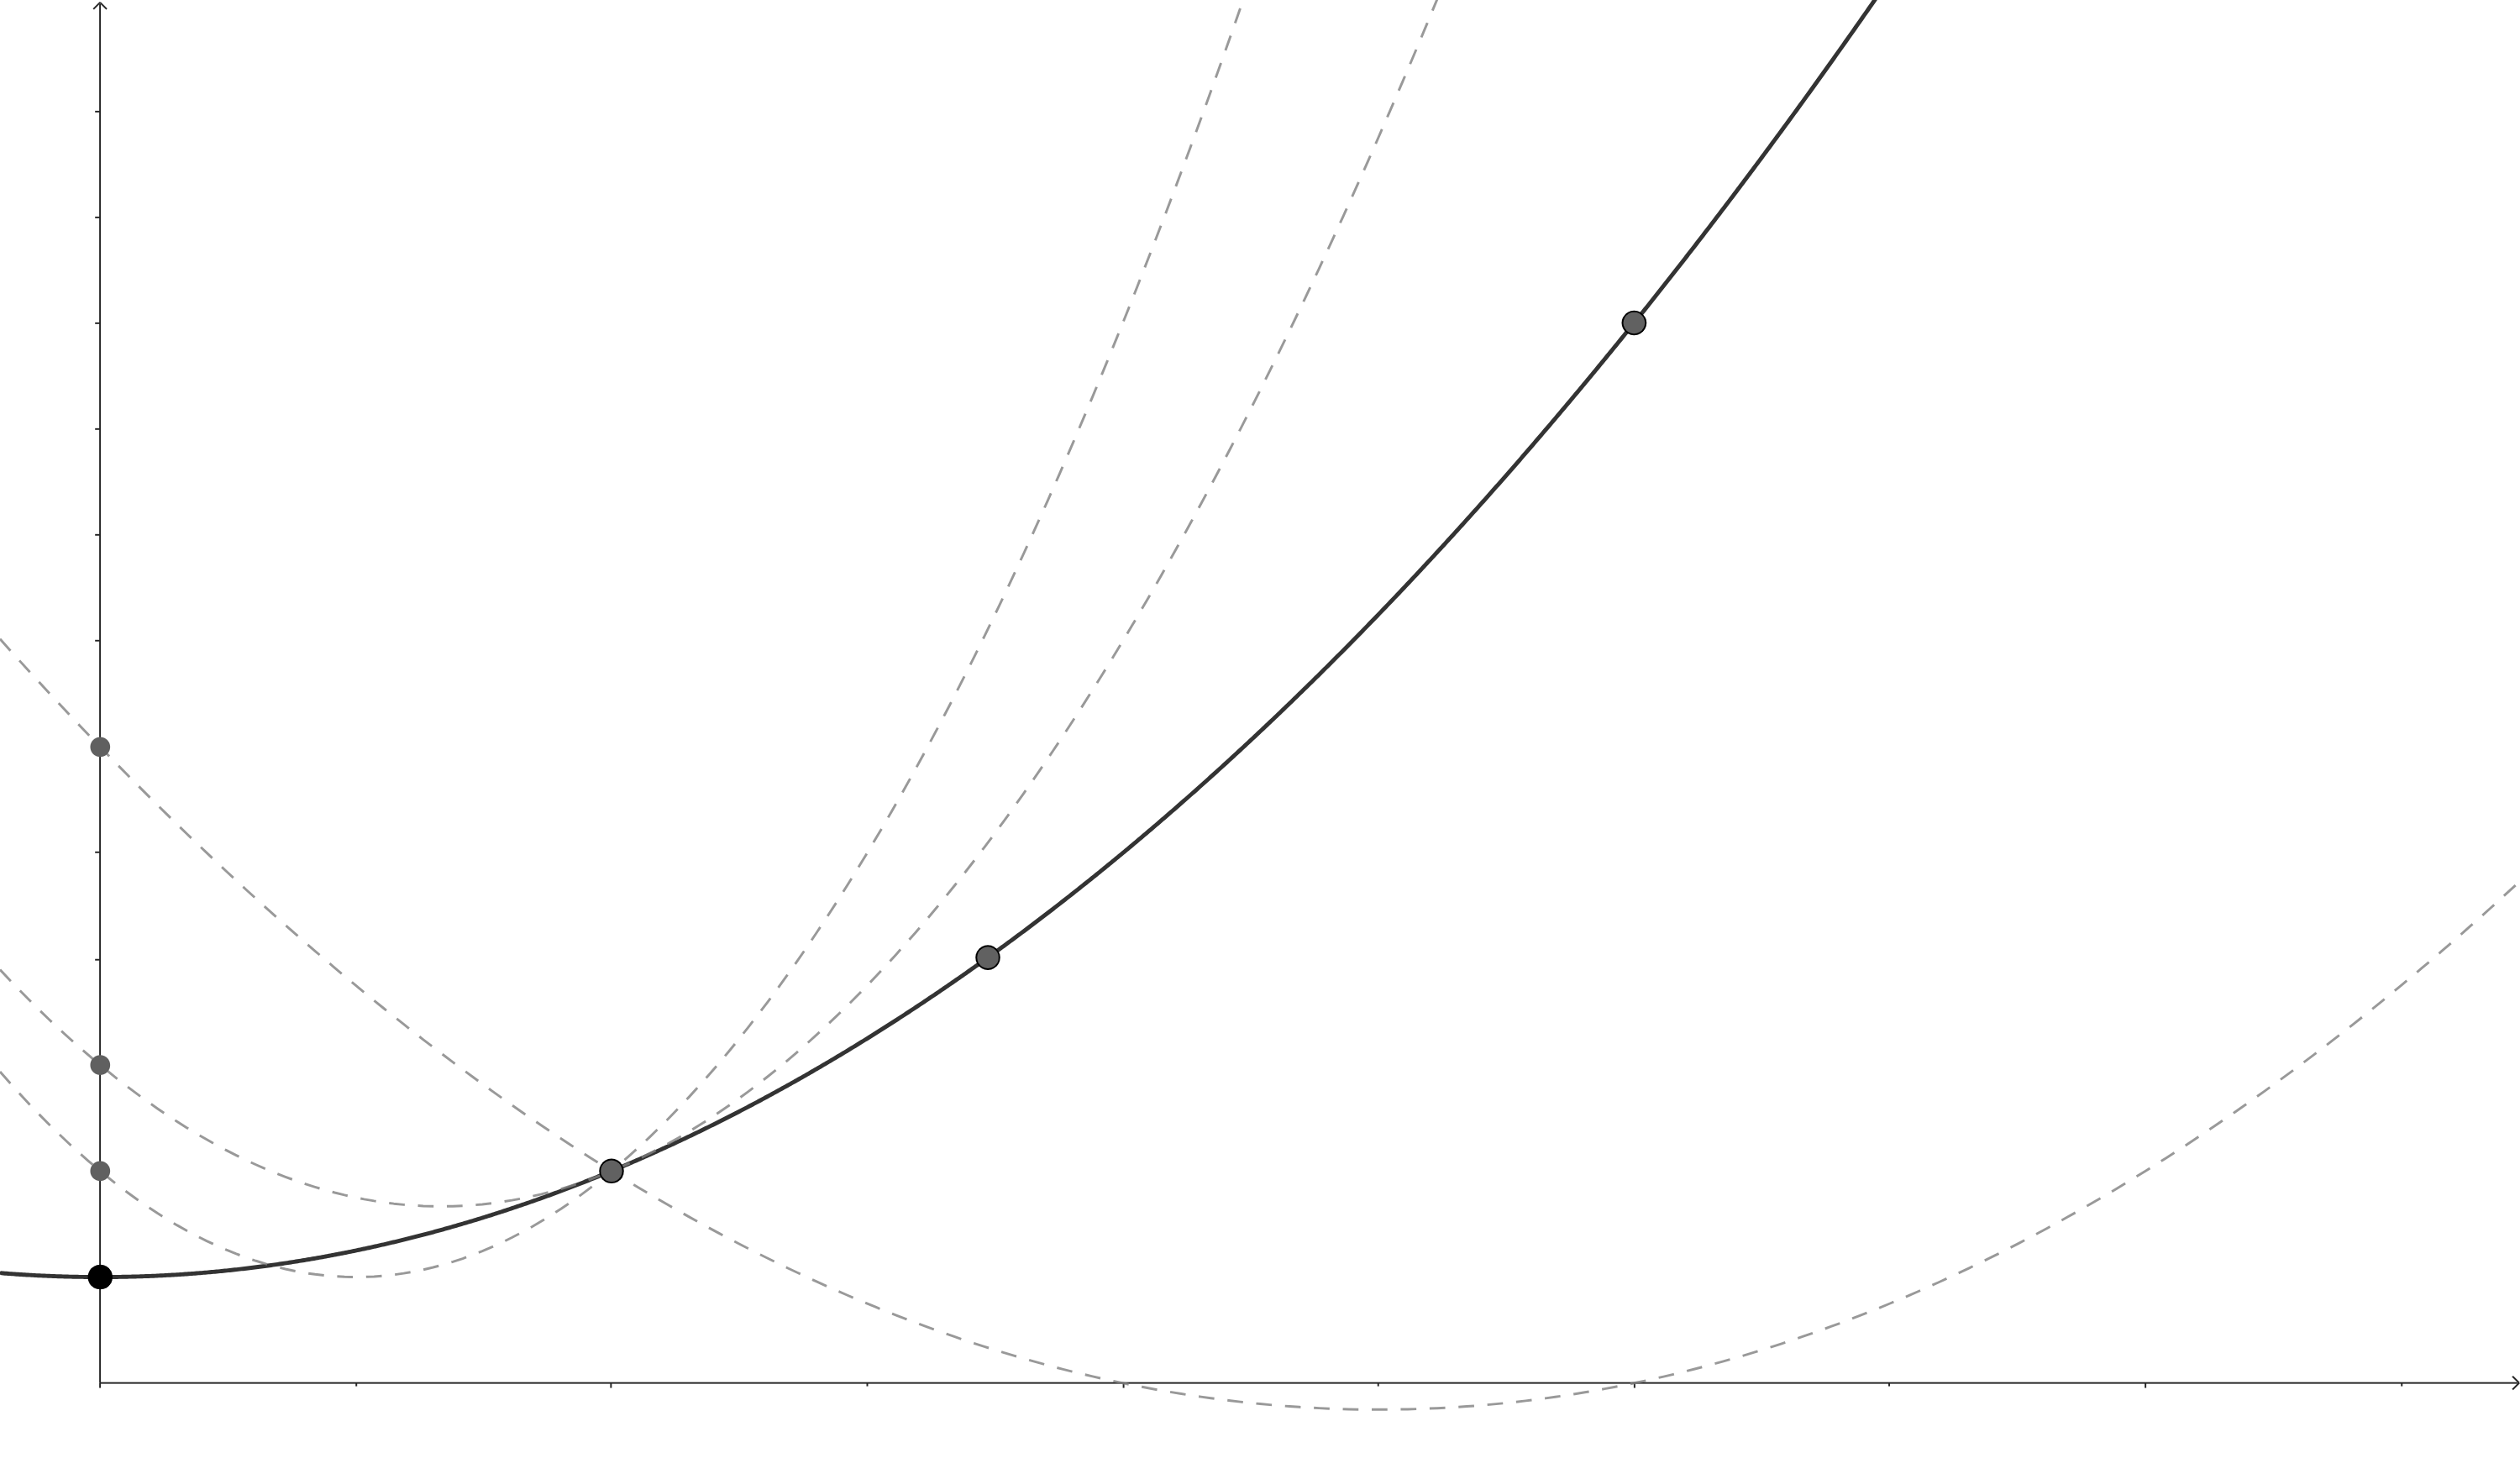
\includegraphics[width=0.8\textwidth]{images/shamir.png}
  \caption{Visualization of the Shamir's polynomial based secret sharing scheme. The dark line shows the specific sharing instance for a secret $s$ and a threshold $\ell=2$. With three shares, the secret can be reconstructed by interpolating the polynomial from the shares. However, with one or two shares, the reconstructed polynomial is not unique as we can see from the dotted lines.}\label{fig:shamir}
\end{figure}

\subsection{Secure Multi-Party Computation}\label{sec:mpc}

Secure Multi-Party Computation (MPC) refers to a cryptographic protocol enabling multiple parties to jointly compute a function $f$ represented by a circuit $C$, ensuring that no information about the individual inputs is revealed beyond what can be inferred from the output of $C$. In the following, sections we will denote a MPC protocol by $f$ for an $n$-party functionality $f(x, w_1, \dots, w_n)$, a public input $x$ and secret inputs $w_i$ of the party $P_i$. The goal is to compute the function $f$ on the inputs of the $n$ parties while upholding the following properties~\cite{cramer2015secure}

\begin{definition}[Correctness]\label{def:mpc-correctness}
  We say that $\Pi$ realizes a deterministic $n$-party functionality $f(x, w_1, \dots, w_n)$ with perfect (resp., statistical) correctness if for all inputs $x, w_1, \dots, w_n$, the probability that the output of some player is different from the output of $f$ is $0$ (resp., negligible in $k$), where the probability is over the independent choices of the random inputs $r_1, \dots, r_n$.
\end{definition}

\begin{definition}[Privacy]\label{def:mpc-privacy}
  The protocol ensures that no party learns anything about the inputs of the other parties beyond what can be inferred from the output of the function.
\end{definition}

\begin{definition}[$\ell$-privacy]\label{def:mpc-ell-privacy}
  The MPC protocol has privacy up to $\ell$ malicious parties.\footnote{Most often achieved by using a $(\ell + 1, N)$-threshold secret sharing scheme \autoref{def:mpc-ss-threshold}}
\end{definition}

In terms of security needed for the SD-in-the-Head protocol, we define the following security requirements for the MPC protocol $f$

\begin{itemize}
  \item \textbf{Semi-honest security}: The protocol is secure against semi-honest adversaries, where parties follow the protocol but may attempt to learn information from the messages they receive.
  \item \textbf{Low-threshold security}: The protocol is secure against a coalition of up to $\ell$ parties, where $\ell$ is the threshold. This is also known as a $\ell$-private MPC protocol.
\end{itemize}

In order to prove the validity of a MPC protocol that have been run in the head, we define the following notion of \textit{consistency}~\cite{ishai2007zero}.

\begin{definition}[MPC view]\label{def:mpc-view}
  We denote the view $V_i$ of a party $P_i$ in the protocol as $(i, x, r_i, w_i, (m_1, \dots, m_j))$ where $r_i$ is the randomness used by $P_i$, $w_i$ is the secret share, and $(m_1, \dots, m_j)$ is the messages received by $P_i$ in the first $j$ rounds of the protocol. Note that the messages sent by the parties can be inferred from the $V_i$ by invoking $\Pi$.
\end{definition}

\begin{definition}[Consistent views]\label{def:mpc-consistent-view}
  We say that a pair of views $V_i, V_j$ are consistent (with respect to the protocol $\Pi$ and some public input $x$) if the outgoing messages implicit in $V_i, x$ are identical to the incoming messages reported in $V_j$ and vice versa.
\end{definition}

\begin{lemma}[Local vs. global consistency]\label{lem:consistency}
  Let $\Pi$ be an $n$-party protocol as above and $x$ be a public input.
  Let $V_1, \dots, V_n$ be an $n$-tuple of (possibly incorrect) views. Then all pairs of views $V_i, V_j$ are consistent with respect to $\Pi$ and $x$ if and only if there exists an honest execution of $\Pi$ with public input $x$ (and some choice of private inputs $w_i$ and random inputs $r_i$) in which $V_i$ is the view of $P_i$ for every $1 \leq i \leq n$.
\end{lemma}

\textbf{Proof of \autoref{lem:consistency}} The \textit{if} direction is trivial and follows from \autoref{def:mpc-view} and \autoref{def:mpc-consistent-view}.
The \textit{only if} direction is shown by the following. Consider $n$ pairwise consistent views $V_1, \dots, V_n$ \autoref{def:mpc-view}. Let us define an MPC protocol $\Pi$ by its \textit{next sent message} function $\Pi_j(i,x,w_i,r_i, (m_1, \dots, m_j)) = m_{j+1}$. The pairwise consistency, \autoref{def:mpc-consistent-view} and $\Pi_j$ implies, by induction that after $d$ rounds, that the actual view of all parties $P_i$ is the same as the view of $P_i$ in the first $d$ rounds. It follows that the views $V_i, \dots, V_n$ are consistent with the full execution of $\Pi$. \qed

\subsection{Zero-Knowledge Proofs}\label{sec:zk}
This section will give a brief introduction to \textit{two-party interactive} Zero-Knowledge (ZK) schemes for a \textit{prover} and a \textit{verifier}. The intuition behind a Zero-Knowledge proof of knowledge is that the prover can convince the verifier that they know a secret $w$, such that $x$ is true, without revealing the secret $w$ to the verifier. This could be someone wanting to prove that they are above the age of 18 without revealing their age. We denote a ZK $\Pi_{\mathcal{R}}$ for some NP relation $\mathcal{R}(x, w)$. Let $x$ be a public statement in \textbf{NP} and $w$ be a witness such that $(x, w) \in \mathcal{R}$~\cite{feneuil2023threshold}.
\todo{Use the ivan reference}

\begin{definition}
  Let $x$ be a statement of language $L$ in \textbf{NP}, and $W(x)$ the set of witnesses for $x$ such that the following relation holds:
  \begin{align*}
    \mathcal{R} = \{(x, w)\; x \in L, w \in W(x)\}
  \end{align*}
\end{definition}

\section{Syndrome Decoding Problem}\label{sec:syndrome}

The SD-in-the-Head protocol is built on the computational hardness of the Syndrome Decoding (SD) problem for random linear codes over a finite field (see \autoref{sec:gf256}). This protocol uses a variant of the SD problem, referred to as the \textit{coset weights} problem, first introduced by Berlekamp and McEliece in 1978~\cite{berlekamp1978inherent}. The problem is defined as follows:
\begin{definition}\label{def:syndrome}
  Given $H \in \mathbb{F}^{(m-k)\times m}_q$ and $y \in \mathbb{F}^{m-k}_q$. The problem is to find $x \in \mathbb{F}^m_q$ s.t.\ wt$(x) \leq w$ such that $Hx = y$.
\end{definition}
Generating such an instance is straightforward: one can construct a uniformly random parity-check matrix $H$ and a codeword $x$ (with $wt(x) \leq w$), and then compute the syndrome $y = Hx$. In the SD-in-the-Head protocol, the values of the matrix $H$ and the syndrome $y$ are elements of the finite field $\mathbb{F}_q$ explained previously in \autoref{sec:gf256}. The SD problem is well-known to be NP-complete for random instances~\cite{berlekamp1978inherent} also referred to as the general decoding problem.To illustrate the computational difficulty, solving the problem using brute force would require $O(\binom{m}{w} q^w)$ operations, which is computationally infeasible for large $m$ and $k$.

\subsubsection{Standard form of the parity-check matrix}\label{sub:standard_form_of_the_parity_check_matrix}
To improve the performance and reduce the key size of the protocol, its possible to utilize the fact that the matrix $H$ can be in standard form. $H = (H'|I_{m-k}) $ Where $H' \in \mathbb{F}^{(m-k)\times k}_q$, and $I_{m-k}$ is the identity matrix of size $m-k$. This allows for the following representation of the syndrome:
\begin{equation}
  y = Hx = H'x_A + x_B\label{eq:standard_form_of_the_parity_check_matrix}
\end{equation}
with $x = (x_A | x_B)$. This improves the performance of the algorithms used in the SD-in-the-Head protocol in the following ways
\begin{itemize}
  \item At the MPC layer, we only need to reveal one share $x_A$. Due to the fact that the other share $x_B$ can simply be recomputed by $x_B = y - H'x_A$.
  \item By linearity of the above relation one only needs to send $x_A$ in order to recover $Hx = H'x_A + x_B$ the Syndrome decoding instance. So from a sharing of $x_A$ one can check the correctness of the SD instance.
\end{itemize}

\subsubsection{Polynomial representation of SD}\label{sec:polynomial_representation}

The SD-in-the-Head MPC protocol must prove that the SD problem $ y = Hx $ is satisfied. As outlined in \autoref{def:sdith-mpc}, the shared input $\sh{x_A}$ is provided to the MPC protocol. Consequently, the correctness of the initial statement $ y = Hx $ follows directly~\cite{feneuil2022syndrome}.

In addition to this, we need to verify that the Hamming weight condition $ \text{wt}(x) \leq w $ holds. To achieve this, the prover constructs three polynomials $ S $, $ Q $, and $ P $, alongside one public polynomial $ F $. These polynomials play a critical role in ensuring the weight condition is satisfied while preserving the zero-knowledge property of the protocol. The polynomials are defined as follows:

\begin{definition}[SD-in-the-Head polynomials representation]\label{def:sdith-polynomials}
  Let $f_1,\dots, f_q$ denote all the elements of $\mathbb{F}_q$ and $x\in \mathbb{F}^m_q$ is a binary vector with hamming weight $wt(x) /leq w$, then the polynomials are defined as:
  \begin{itemize}
    \item $S\in \mathbb{F}_q[X]$ is the Lagrange interpolation of the coordinates of $x$, such that it matches $S(f_i) = x_i$ for $i\in [1:m]$ and has degree $\text{deg}(S) \leq m-1$
    \item $Q\in \mathbb{F}_q[X]$ is defined by $Q(X) = \prod_{i\in E}(X - f_i)$. $E \subset [1:m]$ with order $|E| = w$, such that $E$ contains the non-zero coordinates of $x$. $Q$ has degree $\text{deg}(Q) = w$.
    \item $P\in \mathbb{F}_q[X]$ is defined as $P = S\cdot Q/F$ and has degree $\text{deg}(P) \leq w-1$. By definition the polynomial $F$ divides $S\cdot Q$.
    \item $F\in \mathbb{F}_q[X]$ is the \textit{vanishing polynomial} of the set ${f_1, \dots, f_m}$ also defined as $F(X) = \prod_{i\in [1:m]}(X - f_i)$ and has degree $\text{deg}(F) = m$.
  \end{itemize}
\end{definition}

We can now look at the relation
\begin{equation}
  \centering
  S\cdot Q = P\cdot F\label{eq:polynomial_representation}
\end{equation}

If we look at the left-hand side, which has the following property by design $S\cdot Q(f_i) = 0 \ \forall\ f_i \in [1:m]$. This comes from the fact that the polynomial $S(f_i) = 0$ whenever $x_i = 0$, as it is the lagrange interpolation of $x$. Furthermore, the polynomial $Q(f_i)$ is zero whenever $f_i$ is a non-zero coordinate of $x$, which follows from the definition of $Q$.

For the right-hand side, the polynomial $F$ is the vanishing polynomial for the set ${f_1, \dots, f_m}$, so $F(f_i) = 0\ \forall\ f_i \in [1:m]$. The polynomial $P$ is needed to match the degree of $S \cdot Q$. As the degree of $F$ is $m \leq \text{deg}(S\cdot Q) \leq m + w - 1$.

It is now apparent that if the prover can convince the verifier that they know of polynomials $P,Q$ such that $S\cdot Q = F \cdot P = 0$ at all points $f_i \in [1:m]$. The following must hold, either $S(f_i) = x_i = 0$ or $Q(f_i) = 0$. However, the polynomial $Q$ can be zero in at most $w$ points based on the degree, this means that S is non-zero in at most $w$ points, based on the construction, which in turn implies that $\text{wt}(x) \leq w$.

With this, we can define the soundness of the language for ZKP as follows:
\begin{equation}
  wt(x) \leq w \Leftrightarrow \exists P,Q \text{  with  }\text{deg}(P)\leq w-1\text{  and  }\text{deg}(Q) = w\text{ s.t. \autoref{eq:polynomial_representation} holds}\label{eq:soundness}
\end{equation}

\subsubsection{False positive probability}\label{sub:equality_test}
The equality test from \autoref{eq:polynomial_representation} has a small probability of false positives, denoted $p$. To reduce this probability, the relation is evaluated at random points $\{r_k \in \mathbb{F}_q\}_{k\in[t]}$. By Schwartz-Zippel \autoref{lem:schwartz}, the probability of a false positive is bounded by $p \leq \frac{t}{q}$, where $q$ is the size of the finite field $\mathbb{F}_q$. In short, this makes it unlikely that the relation will hold for all points $r_k$ if the relation is not sound according to \autoref{eq:soundness}. Furthermore, we can tweak the parameters $t$ and $q$ to reduce $p$.

\begin{lemma}[Schwartz-Zippel]\label{lem:schwartz}
  For a non-zero polynomial $P \in \mathbb{S}[X]$ of degree $d \geq 0$. Let $\mathbb{R}$ be a finite subset of $\mathbb{S}$ and set of random points $[r_1, \dots, r_n] \in \mathbb{R}$, the probability that $\Pr[P(r_1, \dots, r_n) = 0] \leq d/|\mathbb{R}|$.
\end{lemma}

\subsubsection{Avoiding interpolations for $S$}\label{sec:syndrome-avoid-interpolation}
Recall the sharing of the witness $\sh{x_A}$ for $x = (x_A | x_B)$ detailed in \autoref{sec:syndrome}. We would have to use interpolation to compute $\sh{S}$ for each share $\sh{x_A}$. However, interpolation is computationally expensive. To mitigate this, we redefine the SD instance as follows:

\begin{definition}[Redefined SD instance $y = Hx$]
  Let $s$ represent the coefficients of the polynomial $S$ in \autoref{eq:polynomial_representation}, and let $V$ be a matrix such that:
  \begin{align*}
    S = \text{Lagrange Interpolation}(x) \Leftrightarrow s = Vx.
  \end{align*}
  The SD instance is then redefined as:
  \begin{align*}
    y = HVx.
  \end{align*}
\end{definition}

This redefinition preserves the security properties of the original SD problem, as the linear code $\mathcal{C}_{HV}$ remains uniformly random. This is due to the randomness of $\mathcal{C}_H$ and the invertibility of $V$.

With this modification, we can replace the sharing $\sh{x_A}$ by representing $s = (s_A \mid s_B) = Vx$. The parties can then compute $\sh{s_B}$ and $\sh{s}$ from the sharing of $\sh{s_A}$ using:
\begin{align*}
  \sh{s_B} = y - H'\sh{s_A}.
\end{align*}

\section{MPC-in-the-Head}\label{sec:mpcinth}

The SD-in-the-Head protocol construction is based on the \textit{Multi-Party Computation in the Head} (MPCitH) framework. In this section we will give an introduction to the framework and how it can be used to construct ZK proofs, which in turn can be combined with the Fiat-Shamir heuristic to create a signature scheme.

The MPC-in-the-Head (MPCitH) framework, introduced by~\cite{ishai2007zero}, builds upon these techniques to construct generic zero-knowledge protocols (ZK). A ZK protocol allows a \textit{prover} to convince a \textit{verifier} of the validity of a statement without revealing any information about the inputs to the statement. The framework provides a versatile method of constructing protocols that are quantum safe as its security relies on assumptions that are still believed to be quantum secure. Namely, commitment schemes and hash functions~\cite{feneuil2023threshold} which have no known quantum algorithms that break their security.

We will describe the basic construction suggested by Ishai et al~\cite{ishai2007zero}. For now, we will only consider an underlying semi-honest MPC protocol $f_{add}$ for $N$ parties with $N-1$ secrecy based on \textit{additive} secret sharing \autoref{sec:additive-sss}.

\begin{protocol}\label{def:mpcinth_basic}
  Given $f_{add}$ a ZK relation $\mathcal{R}$ for some public statement $x$, and a witness $w$ (\autoref{sec:zk}).
  Let $w_i$ be an additive secret share of $\sh{w}$ for the party $P_i$. Let $f_{add}(x, w_1, \dots, w_n) = \mathcal{R}(x, w)$, i.e. $f_{add}(x,w)$ accepts if $(x,w) \in \mathcal{R}$.

  \begin{enumerate}[parsep=2pt, itemsep=0pt]
    \item The prover builds a random sharing of $\sh{w} = w_1, \dots, w_n$. Then
          \begin{enumerate}[nolistsep]
            \item Simulates the outputs of the MPC protocol $f$ on the inputs $(x, w_1, \dots, w_n)$ and the randomness $r_1, \dots, r_n$.
            \item Prepares views $V_1, \dots, V_n$ of the parties in the protocol $f$.\footnote{Remember that the views include the inputs, randomness and messages received by the parties.}
            \item Commits to each view $V_i$ using a secure commitment scheme, and sends ($\text{Commit}(V_1), \dots, \text{Commit}(V_n)$) to the verifier.
          \end{enumerate}
    \item The verifier picks $\ell$ random distinct indices $i \in [n]$ and sends them to the prover.
    \item The prover opens the corresponding $\ell$ commitments into the views $V_i$ and sends the openings to the verifier.
    \item The verifier accepts if and only if:
          \begin{enumerate}[nolistsep]
            \item\label{prop:mpcinth_commit} The views are valid according to the commitment scheme.
            \item\label{prop:mpcinth_consistent} The views are consistent according to the public input $x$.
            \item\label{prop:mpcinth_knowledge} The views output $1$ according to $\mathcal{R}$ meaning that $\mathcal{R}(x,w) = 1$.
          \end{enumerate}
  \end{enumerate}
\end{protocol}

We see the following properties of the protocol:

\begin{lemma}[Completeness~\cite{ishai2007zero}]\label{def:mpcinth_completeness}
  A boolean function is said to be complete if it depends on all inputs of the function. Given an honest prover, $\mathcal{R}(x,w) = 1$ and the correctness of the MPC protocol $f_{add}$, all outputs of $P_i$ are one and all views are consistent.
\end{lemma}

\begin{lemma}[Zero-Knowledge~\cite{ishai2007zero}]
  The verifier only sees $\ell$ views, and therefore from the definition of the MPC protocol $f_{add}$ learns nothing of the secret witness $w$.
\end{lemma}

We consider soundness of the MPCitH framework. We assume that the verifier accepts the relation $\mathcal{R}(x,w)$ for $x \notin L$ -- i.e. the verifier accepts the relation even though the prover has created a false statement. This means that the prover must have cheated on of two ways. First, the prover may have cheated in the underlying MPC protocol which is defined by the error probability $p_{f_{add}}$.

Secondly, the prover could have tampered with the views. In this, the prover must have corrupted one party and creating a inconsistent view. The probability that the prover succeeds with this is at most $1 / N$. This gives us an overall soundness

\begin{lemma}[Soundness of MPCitH for $f_{add}$~\cite{feneuil2022syndrome}]\label{lem:soundness_mpcinth}
  \begin{align*}
    1 - (1 - \frac{1}{N}) (1 - p_{f_{add}}) = \frac{1}{N} + p - \frac{1}{N} p_{f_{add}}
  \end{align*}
\end{lemma}

The basic MPC-in-the-Head protocol serves as a foundation for constructing zero-knowledge (ZK) proofs for any NP relation and has been demonstrated to yield relatively efficient ZK protocols~\cite{feneuil2022syndrome,baum2020concretely,katz2018improved}. Giacomelli et al. and Chase et al.~\cite{katz2018improved,giacomelli2016zkboo,chase2017post} provided concrete implementations of the \emph{MPC-in-the-Head} approach and observed that employing a 3-party protocol $\Pi$ achieved optimal performance within the space of protocols they analyzed. However, due to the small number of parties, the soundness of the resulting honest-verifier zero-knowledge (HVZK) proof is relatively weak. As a consequence, a large number of parallel repetitions is required to achieve negligible soundness error. This increases the size of the proofs and the communication overhead of the protocols. In this section we will describe a variant of the MPC-in-the-Head protocol which is sound for the addition relation.

\section{MPC Product verification using sacrificing}\label{sec:mpc_sacrificing}

To enhance the performance of MPCitH-based zero-knowledge protocols, Baum and Nof introduced a variant of the framework built around a specialized MPC protocol. This protocol efficiently verifies a product relation between three values, $  a \cdot b = c  $. Their contributions significantly improved the efficiency of MPCitH-based zero-knowledge protocols and laid the foundation for the SD-in-the-Head protocol, which is designed to prove the SD relation (\autoref{sec:syndrome}).

The underlying MPC protocol is based on arithmetic circuits, where addition operations are straightforward to perform using any $ + $-homomorphic secret sharing scheme. However, performing multiplication -- which is required for the product relation -- is significantly more challenging. In this section, we describe the techniques and mechanisms used to address this challenge. The simplest idea would be to verify the relation by simply computing the product. A common technique is to use Beaver triples.

\begin{definition}[Beaver triple~\cite{Beaver1992efficient}]\label{def:Beaver}
  A Beaver triple is a tuple $ (a, b, c) $ such that $ a \cdot b = c $, where $ a, b, c \in \mathbb{F}_q $.
\end{definition}

\begin{protocol}[MPC Multiplication using Beaver triples]\label{def:Beaver-multiplication}
  Given a $+$-homomorphic additive secret sharing scheme and a preprocessed random Beaver triple $\sh{a}, \sh{b}, \sh{c} $, the parties do the following:
  \begin{enumerate}
    \item The parties compute $ \sh{\alpha} = \sh{x} - \sh{a} $ and $ \sh{\beta} = \sh{y} - \sh{b} $.
    \item The parties run $ \text{open}(\sh{\alpha}) $ and $ \text{open}(\sh{\beta}) $ to obtain $ \alpha $ and $ \beta $.
    \item Each party computes $ \sh{z} = \sh{c} - \alpha \cdot \sh{b} - \beta \cdot \sh{a} + \alpha \cdot \beta $.
  \end{enumerate}
\end{protocol}


The above is a well-known technique~\cite{Beaver1992efficient} correctness follows from the fact that
\begin{align*}
  \sh{z} & = \sh{c} - \alpha \cdot \sh{b} - \beta \cdot \sh{a} + \alpha \cdot \beta        \\
         & = \sh{ab} - (x - a) \cdot \sh{b} - (y - b) \cdot \sh{a} + (x - a) \cdot (y - b) \\
         & = \sh{xy}
\end{align*}

Proposals for zero-knowledge proofs -- such as the \textit{Cut-and-Choose} protocol~\cite{katz2018improved,baum2020concretely} -- utilize \autoref{def:Beaver-multiplication}, combined with preprocessing techniques, to achieve promising results\footnote{See \autoref{sec:zk-cut-and-choose}}. Building upon these protocols, Baum and Nof~\cite{baum2020concretely} propose a variant that shifts the focus from simulating the computation of a product to simulating the \textit{verification} of the triple relation instead. This verification is achieved by sacrificing another triple, ensuring correctness while improving performance. Consider the following protocol, which is based on the MPC protocol described in~\cite{damgaard2012multiparty}.

\begin{protocol}[Verification of a multiplication triple by sacrificing another]\label{def:sacrifice}
  Given an input triple $(x,y,z) \in \mathbb{F}$ random shared triple $(\sh{a}, \sh{b}, \sh{c}) \in \mathbb{F}$, it is possible to verify the correctness of the statement $z = x \cdot y$ without revealing any information on either of the input. Define \texttt{open} according to \autoref{def:ss-share}.
  \begin{enumerate}
    \item The parties generate a random $\varepsilon \in \mathbb{F}$.
    \item The parties locally set $\sh{\alpha} = \varepsilon\sh{x} + \sh{a}, \sh{\beta} = \sh{y} + \sh{b}$.
    \item The parties run \texttt{open}$(\sh{\alpha})$ and \texttt{open}$(\sh{\beta})$ to obtain $\alpha$ and $\beta$.
    \item The parties locally set $\sh{v} = \varepsilon\sh{z} - \sh{c} + \alpha  \cdot \sh{b} + \beta  \cdot \sh{a} - \alpha  \cdot \beta$.
    \item The parties run \texttt{open}$(\sh{v})$ to obtain $v$ and accept iff $v = 0$.
  \end{enumerate}
\end{protocol}

Observe that if both triples are correct multiplication triples (i.e., $z = xy$ and $c = ab$) then the parties will always accept since

\begin{align*}
  v & = \varepsilon \cdot z - c + \alpha \cdot b + \beta \cdot a - \alpha \cdot \beta                                                     \\
    & = \varepsilon \cdot xy - ab + (\varepsilon \cdot x + a)b + (y + b)a - (\varepsilon \cdot x + a)(y + b)                              \\
    & = \varepsilon \cdot xy - ab + \varepsilon \cdot xb + ab + ya + ba - \varepsilon \cdot xy - \varepsilon \cdot xb - ay - ab           \\
    & = (\varepsilon \cdot xy - \varepsilon \cdot xy) + (ab - ab) + (\varepsilon \cdot xb - \varepsilon \cdot xb) + (ya - ay) + (ba - ab) \\
    & = 0
\end{align*}

\begin{lemma}\label{lem:sacrifice_soundness}
  If $(\sh{a}, \sh{b}, \sh{c})$ or $(\sh{x}, \sh{y}, \sh{z})$ is an incorrect multiplication triple then the parties output \texttt{Accept} in the sub-protocol above with probability $\frac{1}{|\mathbb{F}|}$.
\end{lemma}

\textit{Proof}. Let $\Delta_z = z - x \cdot y$ and $\Delta_c = c - a \cdot b$. If the party accepts, then $v = 0$.
\begin{align}
  v & = \varepsilon \cdot z - c + \alpha \cdot b + \beta \cdot a - \alpha \cdot \beta                           \nonumber             \\
    & = \cdot (xy + \Delta_z ) - (ab + \Delta_c) + (\varepsilon \cdot x + a)b + (y + b)a - (\varepsilon \cdot x + a)(y + b) \nonumber \\
    & = \varepsilon\Delta_z - \Delta_c = 0 \label{eq:sacrifice-proof}
\end{align}

Consider the cause where one of $\Delta_z$ or $\Delta_c$ is zero and the other is non-zero. In this case the verifier will not accept from~\ref{eq:sacrifice-proof}. Otherwise, we require that $\varepsilon = \Delta_c \cdot \Delta_z^{-1}$ which happens with probability $\frac{1}{|\mathbb{F}|}$. \qed

\autoref{def:sacrifice} forms the foundational mechanism underpinning the SD-in-the-Head protocol. While this approach delivers significant improvements~\cite{baum2020concretely,feneuil2022syndrome} in efficiency and soundness for ZK protocols, further advancements can be achieved by revisiting the secret sharing schemes utilized within the MPCitH framework.

\section{Threshold Computation in the Head (TCitH)}\label{sec:threshold-mpc}

A majority of constructions within the MPCitH framework~\cite{baum2020concretely,feneuil2022syndrome,katz2018improved} rely on $ (N-1, N) $ additive secret sharing schemes (SSS). Feneuil and Rivain~\cite{feneuil2023threshold,feneuil2023threshold2} explore the application of threshold secret sharing schemes (\autoref{sub:threshold-sss}). In addition to improving the soundness of the resulting zero-knowledge protocol, their approach reduces the computational overhead: the prover needs to emulate only $ \ell + 1 $ parties, while the verifier needs to verify and emulate just $ \ell $ parties. This optimization delivers significantly improved performance, particularly for low-threshold schemes.

\begin{table}[]
  \centering
  \def\arraystretch{1.5}%  1 is the default, change whatever you need
  \begin{tabular}{cc|c}
    \textbf{} & MPCitH                                  & TCitH                                                      \\ \arrayrulecolor{darkgray}\hline
    Prover    & $ \approx \lambda \frac{N}{\log_2 N}$   & $ \approx \lambda \frac{\ell + 1}{\log_2 \binom{N}{\ell}}$ \\ \arrayrulecolor{lightgray}\hline
    Verifier  & $ \approx \lambda \frac{N-1}{\log_2 N}$ & $ \approx \lambda \frac{\ell + 1}{\log_2 \binom{N}{\ell}}$ \\ \arrayrulecolor{darkgray}\hline
  \end{tabular}
  \caption{Performance for prover and verifier for TCitH compared to MPCitH. I.e. the number of party emulations to achieve a soundness error of $2-\lambda$ (assuming a negligible false positive rate for the underlying MPC protocol). From \cite{feneuil2023threshold}}\label{tbl:tcith-performance}
\end{table}

We define a threshold MPC protocol, $ f_{thr} $, based on a $ (\ell, N) $-private SSS. In the context of the SD-in-the-Head protocol, this can be instantiated with Shamir's Secret Sharing (\autoref{sub:shamir}).

On the other hand, the TCitH model described by~\cite{feneuil2023threshold} results in a slightly larger proof size due to the increased flexibility in the number of input shares the prover must open. While the prover still commits to all input sharings, only a subset of these needs to be opened during the protocol.

To facilitate this, a Merkle Tree Commitment Scheme (\autoref{sub:merkle_tree_prelim}) is employed. This scheme enables the prover to efficiently prove the consistency of a subset of committed inputs by providing additionally the authentication path along with the tree root -- introducing the slight increase in communicational complexity.

\todo{Add protocol here}

\begin{lemma}[Soundness of TCitH based ZK]
  Given a threshold MPC protocol $ f_{thr} $ with threshold $ \ell $ and $ N $ parties, we see a soundness error
  \begin{align*}
    \frac{1}{\binom{N}{\ell}} + p_{f_{thr}} \cdot \frac{\ell \cdot (N - \ell)}{\ell + 1}
  \end{align*}
\end{lemma}

\textit{Proof:} Soundness follows the same principle as before, with a slight modification. First, assume that the MPC protocol has a perfect error rate $  p_{f_{thr}} = 0  $.

\begin{proposition}
  The malicious prover must tamper with exactly $  N - \ell  $ MPC party emulations to successfully cheat the verifier.
\end{proposition}

Consider the case where the malicious prover attempts to cheat on fewer than $  N - \ell  $ parties. In this scenario, at least $  \ell + 1  $ parties have consistent views. Since $  p_{f_{thr}} = 0  $, these consistent views define a valid witness $  w  $ such that $  \mathcal{R}(x, w) = 1  $, by the definition of the MPC protocol. Conversely, if the prover tampers with more than $  N - \ell  $ parties, the verifier will always detect the inconsistency.

Given $  p_{f_{thr}} = 0  $ and the verifier opening $  \ell  $ inputs, the malicious prover can succeed in cheating the verifier with probability at most:
\begin{align*}
  \frac{1}{\binom{N}{\ell}}
\end{align*}

Now, consider the case where $  p_{f_{thr}} \neq 0  $. The malicious prover may exploit the possibility of cheating the MPC protocol itself, resulting in a soundness error of:
\begin{align*}
  \frac{1}{\binom{N}{\ell}} + \left(1 - \frac{1}{\binom{N}{\ell}}\right) \cdot p_{f_{thr}}.
\end{align*}

Finally, the malicious prover could provide an invalid sharing of the input witness $ \sh{w} $. Under such an attack, the final soundness error becomes:
\begin{align*}
  \frac{1}{\binom{N}{\ell}} + p_{f_{thr}} \cdot \frac{\ell \cdot (N - \ell)}{\ell + 1} \geq \frac{1}{\binom{N}{\ell}} + \left(1 - \frac{1}{\binom{N}{\ell}}\right) \cdot p_{f_{thr}}. \qed
\end{align*}

This final step is formally proven in~\cite[p20]{feneuil2023threshold}.
\todo{Should we go over the proof?}

\section{Fiat-Shamir Heuristic}\label{sec:fiatshamir}
To transform any zero-knowledge protocol into a signature scheme, one can use the approach described in~\cite{fiat1986prove}. Here, we outline the general concept.

Zero-knowledge protocols, such as the MPCitH protocols discussed above, depend on the verifier to issue a challenge to the prover. This challenge acts as a source of randomness, which the prover must not control. The original Fiat-Shamir protocol is based on the problem of factoring integers. Nevertheless, the essential method of transforming a zero-knowledge protocol into a signature scheme remains unchanged.

To adapt a zero-knowledge protocol into a signature scheme, the prover must eliminate the verifier's role in providing the randomness. This is achieved by allowing the prover to independently generate the challenge using a pseudo-random function, such as a secure hash function. By modeling the hash function as a random oracle, its security guarantees ensure that the prover cannot manipulate the randomness of the verification challenge. This maintains the fundamental property of zero-knowledge interactive protocols while enabling the transformation into a non-interactive signature scheme.

Within the context of the SD-in-the-Head protocol, the transformation from a ZK to a signature scheme is accomplished by substituting the verifier's challenge with the output of hash functions, where these hash functions take as input the prover's prior communications.

\section{The Rust Programming language}\label{sec:rust}

Before delving into the specifics of our implementation, we need to answer the question: ``Why is Rust a good choice for our implementation?''.

In 2024, the government of the United States of America took a stance on the future of cyber secure programming languages~\cite{whitehouse2024memorysafe}. In their report, they underline the need for secure building blocks when developing secure software. They point to the fact that \textit{Common Weakness Enumeration} (CWE) data highlights \textit{memory safety vulnerabilities} (MSV) as one of the most pervasive classes of vulnerabilities. MSV's exploit how memory can be accessed, written, allocated, or deallocated in ways that are beyond the scope of the program. Common examples of programming languages that are vulnerable include C and C++, which are widely used due to their high performance. To prevent such vulnerabilities, the report emphasizes the importance of using programming languages that inherently provide memory safety and does not require the developers to manually ensure security.

The Rust programming language addresses memory safety through its unique \textit{borrow checker}~\autoref{sec:rustborrow}, which enforces strict rules on how memory is accessed and managed. In the same year as the White House's report, NIST also released their recommendations on \textit{Safer Languages}~\cite{nistsaferlanguages}, which highlighted Rust as a leading choice. Together, these endorsements underscore that Rust is well-suited for implementing a protocol that adheres to modern security standards.

In addition to its focus on safety, Rust benefits from an extensive library of community-maintained documentation and resources~\cite{rustlangRustProgramming,rustlangPerformanceBook,lurklurkEffectiveRust}. These resources provide invaluable support for developers, enabling them to better understand the language's features and effectively utilize its capabilities.

In this section we will give an overview of the key features of the Rust programming language that make it an ideal choice for this project as we aimed to build it robust by leveraging Rust's safety mechanisms, performance optimization capabilities, dynamic language features, and strong testing infrastructure.

\subsection{Cargo - Rust package manager}\label{sec:cargo}
A Rust program, often referred to as a \textit{crate}, is typically compiled using the Rust Compiler with a command such as \texttt{rustc hello.rs}. However, manually managing versions and dependencies can be tedious and error-prone. To simplify this process, Rust provides a \textit{package manager} called Cargo~\cite{rustlangCargo}.

Cargo is a command-line tool -- run through \texttt{cargo} -- that facilitates the management of dependencies, building, testing, and benchmarking of your crate, as well as generating documentation. It is the officially recommended method for managing and building Rust projects.


\subsection{Memory safety}\label{sec:rustborrow} % mut references
Rust guarantees both type safety (\autoref{sub:rusttypes}) and memory safety. While we will not delve into the details, significant progress has been made toward formal proofs of these guarantees~\cite{jung2017rustbelt}. Unlike many other languages that rely on sophisticated garbage collection mechanisms to ensure memory safety, Rust avoids the associated performance overhead through two key features: the \textit{ownership} and \textit{lifetimes}. Along with a compile time functionality called the \textit{borrow checker}, these features ensure the memory safety of Rust programs. While the borrow checker is often the biggest hurdle for new Rust developers, it is also the feature that makes Rust so powerful.

In this section, we will explore the fundamental aspects of how the borrow checker and ownership work. Only the most critical aspects will be discussed, as more comprehensive information is available in the official documentation~\cite{rustlangRustProgramming}.

\subsubsection{Data races vulnerability}
In the section, we consider the problem of \textit{data races}. These are similar to a race condition and cause undefined behavior that in the end can lead to security vulnerabilities. They occur when
\begin{enumerate}[parsep=0pt, itemsep=0pt]
  \item Two or more pointers access the same memory location concurrently.
  \item At least one of the pointers is being used to write to the memory location.
  \item The is no mechanism to synchronize the data access
\end{enumerate}
In Rust, the borrow checker ensures that no data races can occur and it diagnoses them at compile time.

\subsubsection{The Stack and Heap}
First, it is crucial to first grasp the distinction between the stack and the heap. These are two memory management systems available at runtime~\cite[ch.4]{rustlangRustProgramming}, each with unique characteristics and use cases.

\begin{definition}[The Stack]
  The stack stores values in a last-in-first-out (LIFO) order, meaning the last value added is the first to be removed. All data stored on the stack must have a fixed, known size at compile time. This gives the stack its \textit{fixed-sized} structure.
\end{definition}

\begin{definition}[The Heap]
  The heap, in contrast, is more flexible. When you allocate memory for a value on the heap, you request a specific amount of memory, and the heap manager finds a suitable location for it. A helpful analogy for the heap is docking a spaceship on Coruscant: you tell the spaceport how large your ship is, and they assign you to a landing pad that fits your ship's dimensions, noting where you've been docked.
\end{definition}

\subsubsection{Performance versus Dynamism}

Between the two systems, there exists a \textit{performance versus dynamism} trade-off. Consider the following code example:

\begin{minted}{rust}
  let a: Vec<u8> = vec![1, 2, 3];
  let b: [u8; 3] = [1, 2, 3];
\end{minted}

This code demonstrates two data types being allocated. The first, \rust{a}, is a vector type, while the second, \rust{b}, is a fixed-size array type. The vector type is always allocated on the heap, whereas the fixed array is allocated on the stack. Pushing  and accessing the stack is faster than for on the heap. Therefore, keeping values on the stack tends to outperform heap allocations. This is because heap allocation involves searching for a suitable location in memory to store the data. Accessing data on the heap is slower as you have to follow a pointer from the stack to allocated data. Note that there are several optimisations you can do when allocating to the heap, like changing the allocator for specific use cases, instantiating the vector with a capacity or the \rust{SmallVec} that dynamically changes from the stack to the heap when allocation surpasses its defined capacity. See~\cite{rustlangPerformanceBook} for more.

However, the vector type is far more dynamic. For instance, using the \rust{push} method, you can add more elements to a vector, and the allocator will automatically find additional space on the heap if needed. Conversely, stack allocations in Rust require that the size of the data be known at compile time, which imposes significant restrictions on how dynamic your code can be. This limitation became particularly evident when designing around the different category variants in \autoref{sub:categories}. However, this also ensures at compile time that you cannot access memory outside of the stack, a common vulnerability exposed in C and C++.

Additionally, the stack, due to its fixed-size structure, can only hold a limited amount of data. Attempting to allocate more memory than the stack can accommodate results in a \textit{stack overflow} error. In contrast, the heap offers virtually unlimited storage, as it can dynamically allocate memory as required.

\subsubsection{Ownership and Variable scope}
Now that we have given a brief introduction to the memory allocation, we can delve into the \textit{ownership system}. This system is a crucial aspect of Rust's memory management, as it ensures that memory is allocated and deallocated correctly. Ownership in Rust follows three rules
\begin{enumerate}[parsep=0pt, itemsep=0pt]
  \item Each value has an \textit{owner}
  \item There can only be one owner at one time
  \item When a owner goes out of scope, the value will be \textit{dropped}.
\end{enumerate}
First, we consider the \textit{variable scope} in the following example
\begin{minted}{rust}
{
  // d can not be accessed yet because it has not been assigned to the current scope
  let d = "Peace is a lie";
  println!("{d}") // Now we can use d
} // d is dropped here
\end{minted}
In this example, the variable \rust{d} comes into the scope and remains valid until the scope is closed. This is similar to most other programming languages. This works because the string literal \rust{"Peace is a lie"} is of known size and is allocated on the stack, meaning that it can be easily copied on stack and popped when the current scope ends. It also means that while it is efficient and fast, the variable \rust{d} cannot be mutated after the fact.

\subsubsection{Variable and data interaction with \textit{Move}}

To illustrate where Rust differs, we need a data type that is more complex and stored on the heap instead. We will change the example to use a \rust{String} type
\begin{minted}{rust}
  let mut d = String::from("Peace is a lie");
  d.pust_str(", there is only passion."); // We can mutate d
  println!("{d}"); // prints "Peace is a lie, there is only passion."
\end{minted}
A variable instantiated with the \rust{String} type is dynamically allocated on the heap, and a \textit{pointer} is instead saved on the stack. Now consider both types of assignments with a \textit{re-assignment}
\begin{minted}{rust}
  // Case 1: Stack allocated type
  let d = "Through passion, I gain strength"
  let v = d;

  // Case 2: Heap allocated type
  let d = String::from("Through strength, I gain power");
  let v = d;
\end{minted}

For Case 1, if the string literal \rust{d} implements the \textit{Copy} trait. This means that when we assign \rust{let v = d}, its value can copied onto the stack with a negligent performance hit. This means \rust{d} remains accessible after being used or assigned elsewhere because its data was duplicated. Due to the immutability and fixed size of the string literal, this operation is also memory safe.

However, for Case 2; The variable \rust{d} is instead a \textit{pointer} to a heap-allocated string, it resides on the stack but points to data stored on the heap. When \rust{d} is moved to another variable (e.g., \texttt{v}), the pointer itself is transferred to \texttt{v} and the heap-allocated data remains unchanged. Ownership of the pointer is moved to \texttt{v}. This is called a \textit{move}. After the move, \rust{d} is no longer valid, and any attempt to use it would result in a compile-time error.
\begin{minted}{rust}
  let d = String::from("Through strength, I gain power");
  //  ^ move occurs because `d` has type `String`, which does not implement the `Copy` trait
  let v = d;
  //      ^ value moved here
  println!("{d}"); 
  //        ^^^ value borrowed here after move
  // error[E0382]: borrow of moved value: `d`
\end{minted}

\subsubsection{Why the Restriction?}

Allowing \rust{d} to be used after the move could lead to undefined behavior. For one, due to the variable scoping, the runtime would drop the data for both \rust{d} and \rust{v}. As these would be pointing to the same data, this would case a \textit{double free} memory safety bug. Furthermore, if multiple pointers were allowed to simultaneously access or modify the heap-allocated data, it could result in data races. To avoid such risks and ensure memory safety, Rust enforces its ownership rules. If you need to continue using \rust{d} after a move, you must explicitly \textit{clone} the heap data before transferring ownership. This approach encourages developers to carefully manage how data is accessed and modified, promoting safe and predictable memory usage.

\subsubsection{Functions and ownership}\label{sub:rustlifetimes} % (fold)
Now that we have covered the basics of ownership, we explore how it interacts with functions. When passing a value to a function, the function takes ownership of the value. This means that the function takes over managing the \textit{lifetime} of the value, ensuring that it is not used after the function call, unless it is copied.
\begin{minted}{rust}
  // Case 1: Stack allocated type
  fn makes_copy(some_integer: i32) { // some_integer comes into scope
    println!("{some_integer}");
  } // Here, some_integer goes out of scope. Nothing special happens.

  // Case 2: Heap allocated type
  fn takes_ownership(some_string: String) { // some_string comes into scope
    println!("{some_string}");
  } // Here, some_string goes out of scope and `drop` is called.
    // The memory on the heap is freed.
\end{minted}

In Case 1, again the structure of the stack and known compile time size, nothing special needs to happen. However, in Case 2, the function \rust{takes_ownership} takes ownership of the \rust{String} value \rust{some_string}. When the function ends, the \rust{String} value is dropped, and the memory on the heap is freed. This is because the function takes ownership of the value, and the value is no longer valid after the function call.

However, a function can also take ownership of a value. Here's an example:
\begin{minted}{rust}
  fn main() {
    let d = String::from("hello");
    let (v, len) = calculate_length(d);
    println!("The length of '{v}' is {len}."); // v is valid
    println!("The length of '{d}' is {len}."); // d is not valid
    //                        ^ value borrowed here after move
    // error[E0382]: borrow of moved value: `d`
  }

  fn calculate_length(s: String) -> (String, usize) {
    let length = s.len();
    (s, length)
  }
\end{minted}
The function \rust{fn calculate_length()} takes a pointer and the ownership of the \rust{String} value \rust{d}. It returns the same pointer and ownership of the value along with the computed value. Notice that the ownership of the value works the same as it did before with variable assignment. The function \rust{calculate_length} takes ownership of the value, and \rust{d} is no longer valid after the function call.


\subsubsection{Borrowing with references}
However, often it is tedious to keep transferring ownership of values, whenever they need to be used in a function. So how can we avoid this boilerplate of returning ownership? Rust provides a way of avoiding this transfer of ownership by using \textit{references}. References allow you to \textit{borrow} the value without taking ownership of it. This is done by using the \rust{&} symbol. Consider the example
\begin{minted}{rust}
  fn main() {
    let d = String::from("hello");
    let len = calculate_length(&d);
    println!("The length of '{d}' is {len}."); // d is valid
  }

  fn calculate_length(s: &String) -> (String, usize) {
    //                   ^ the function takes a reference to a String with the `&` symbol
    s.len()
  }
\end{minted}

In this way, the function variables \rust{s} never takes ownership of \rust{d}, meaning that it is not dropped when the function call ends. We call the action of creating a reference \textit{borrowing}.

\subsubsection{Mutable references}
However references have their limitations. The reference is immutable, meaning that we cannot modify \rust{s}. If we wanted to modify the value, we would need to use a \textit{mutable reference}.

\begin{minted}{rust}
  fn main() {
    let mut d = String::from("hello");
    modify(&mut d);
  }
  
  fn modify(s: &mut String) {
      s.push_str(", world");
  }
 \end{minted}

With the \rust{&mut} annotation we tell the compiler that we want to modify the value. This is a powerful feature, but it comes with restrictions. If you have a mutable reference to a value, you can have no other references to that value to prevent data races.
\begin{minted}{rust}
  let mut s = String::from("hello");

  let r1 = &s;
  //       ^^^^^^ immutable borrow occurs here
  let r2 = &mut s;
  //       ^^^^^^ mutable borrow occurs here

  println!("{}, {}", r1, r2);
  //                 ^^ immutable borrow later used here
  // error[E0502]: cannot borrow `s` as mutable because it is also borrowed as immutable
\end{minted}
The compiler eases these restrictions as it can determine the lifetime of the references. Consider the following example
\begin{minted}{rust}
  let mut s = String::from("hello");

  let r1 = &s; // no problem
  let r2 = &s; // no problem
  println!("{r1} and {r2}");
  // variables r1 and r2 will not be used after this point

  let r3 = &mut s; // no problem
  println!("{r3}");
\end{minted}
The last borrow is valid because the previous borrows are no longer in scope. The compiler can determine that the borrows will not be used after the last borrow.

\subsubsection{Lifetimes}
The \textit{lifetime} of a value on the stack refers to the period during which the value is guaranteed to remain valid within its scope. In most cases, developers do not need to actively manage lifetimes, as the compiler can infer them automatically. A value's lifetime begins when it is assigned ownership and ends either when it is dropped or when its ownership is transferred.
\begin{minted}{rust}
  let r: &Item;
  {
    let item = Item { contents: 42 };
    //  ^^^^ binding `item` is declared here
    r = &item;
    //  ^^^^^ borrowed value does not live long enough
  }
  println!("r.contents = {}", r.contents);
  //                          ^^^^^^^^^^ borrow later used here
  // error[E0597]: `item` does not live long enough
\end{minted}
While the Rust compiler, most often can infer the lifetime of a value it can sometimes be necessary to explicitly define the lifetime. This is done by using the \textit{lifetime annotation} \rust{'a}. This is most often used when working with references in structs or functions.
\begin{minted}{rust}
  pub fn find(haystack: &[u8], needle: &[u8]) -> Option<&[u8]> {
    //                  -----          -----            ^ expected named lifetime parameter
    // ...
  } // error[E0106]: missing lifetime specifier
\end{minted}
In this example, there are two choices for the output lifetime for the reference returned by the function. The compiler cannot infer which lifetime to use, so it requires the developer to specify it. This is done by adding the lifetime annotation to the function signature.
\begin{minted}{rust}
  pub fn find<'a, 'b>(h: &'a[u8], n: &'b[u8]) -> Option<&'a[u8]> {
    // ...
  }
\end{minted}
In the example above we have used the \rust{<'a,'b>} to define that the function accepts 2 generic lifetimes $'a$ and $'b$. These can now be used on the signature of the function to ensure that the lifetime of $h$ is $'a$. Allowing the compiler to easily analyze if the reference being passed as $h$ lives long enough.
Furthermore, the compiler can determine that the lifetime of the output reference is the same as the input reference \rust{haystack}.

\subsubsection{Conclusions on Memory Safety in Rust}
This overview only scratches the surface of the power and features that Rust offers. However, it provides a brief introduction to the core features that make Rust a powerful programming language for developing secure and high-performance software. As mentioned, Rust comes with a steep learning curve, but it is supported by a large and active community that offers extensive documentation and resources. We suggest that the reader explore the official Rust Book~\cite{rustlangRustProgramming} or its community made books, like \textit{Effective Rust}~\cite{lurklurkEffectiveRust} and \textit{The Rust Performance book}~\cite{rustlangPerformanceBook}.

\subsection{Correctness (Types, Testing and Errors)}
When creating and iterating on software, it is crucial that you develop in a way that you can continually deliver functional and correct code. There are many patterns that help ensuring this. Rust provides several. In this section we will describe two -- Types and Automated tests.

\subsubsection{The Type System}\label{sub:rusttypes}
Every value in Rust has a \textit{data type}. Programs written in Rust are \textit{statically typed}, meaning the type of each value must be determined at compile time. The type informs the compiler about what operations the value supports and helps catch errors before they reach runtime~\cite[ch.3.2]{rustlangRustProgramming}. Rust's compiler often infers types automatically, but if it cannot, you must explicitly annotate the type of the value. Consider the following example:

\begin{minted}{rust} 
  let guess: u32 = "42".parse().expect("Not a number!"); 
\end{minted}

Here, the \rust{parse} function requires the annotation of the variable \rust{guess} to determine how the string should be parsed. Additionally, if you annotate \rust{guess} with a type that does not implement the \rust{parse} function for strings, the compiler will produce an error. This strict type system ensures that Rust minimizes the possibility of writing incorrect code -- at least in terms of the bounds of the language. While Rust enforces correctness in type usage, ensuring that a program operates semantically as intended, such as adhering to a protocol specification, often requires additional validation methods.

\subsubsection{Automated Testing}
Say that you are implementing field arithmetic -- \textit{funny enough, we needed to do exactly that!} -- you would want your impletation to follow the properties that define the field. For example \textit{associativity over addition}
\begin{align}
  a + (b + c) = (a + b) + c
\end{align}
Such a property is hard to enforce using the type system. However, it is possible to enforce it using \textit{automated testing}. Consider the following examples
\begin{minted}{rust}
  // gf256.rs

  fn gf256_add(a: u8, b: u8) -> u8 {
    a ^ b
  }

  #[cfg(test)]
  mod arithmetic_tests {
    use super::*
    
    #[test]
    fn test_add_associativity() {
      let a = 3;
      let b = 4;
      let c = 5;

      assert_eq!(
        gf256_add(gf256_add(a, b), c), 
        gf256_add(a, gf256_add(b, c))
      );
    }
  }
\end{minted}
This is a simple example of the features that Rust provides that to support automated testing. First we create an internal module \rust{mod arithmetic_tests}. Note the annotation, \mintinline{rust}|#[cfg(test)]|. This ensures that the module is only included when running tests and not in the final production code.

Individual tests are made using the \mintinline{rust}|#[test]| and a function. Then we can use the macro \rust{assert_eq!()} to test whether that our property is upheld.

To run the tests in our implementation you simply run the following
\begin{minted}{bash}
  $ cargo test
  running 1 test
  test gf256::arithmetic_tests::test_add_associativity ... ok
\end{minted}
Crucially, this test allows us to continue developing or optimising the finite field while rerunning the tests to verify that the property remains valid. The more rigourous we test our function, the easier we can debug issues or bugs that may arise.

Writing good tests is a subject extensive enough to warrant its own discussion, and delving into the theory behind it is beyond the scope of this report. From the outset, we designed our implementation with testing in mind. This approach ensures that we can iteratively develop each module and confirm that it adheres to theoretical expectations and the given specification.

\subsubsection{Error handling}\label{sub:rusterror} % https://www.lurklurk.org/effective-rust/panic.html
Testing that functions return the correct values based on \textit{correct} inputs are a crucial part of ensuring correctness. But what happens if you have unexpected inputs? For example on the inputs a user to a CLI\@? This can lead to errors. So how do Rust allow us to deal with errors? There are two ways:
\begin{itemize}
  \item Using a \rust{panic}: Stopping the execution of the program.
  \item Returning a \rust{Result<T, Err>}: A type that wraps the return value with an error value allowing the caller to handle the error.
\end{itemize}
So when is it appropriate to use a panic? The Rust book~\cite[ch.9.3]{rustlangRustProgramming} provides a good guideline for when to use panic.
The general rule is that, if your code would end up in a bad state from which it can not recover it should panic. Everywhere else, you should return a \rust{Result} type. In this way the caller can handle the error in the appropriate way for their use case.
\begin{minted}{rust}
  fn sign(message: &[u8], secret_key: &[u8]) -> Result<Vec<u8>, Error> {
    if secret_key.len() == 0 {
      return Err(Error::SigningError);
    }
    ... code that signs the message ...
    Ok(signature)
  }

  fn main() {
    let message = b"Hello, World!";
    let sk = b"...";
    let signature = sign(&message, &sk);

    // You can match on the result to handle the error
    match signature {
      Ok(signature) => println!("Signature: {:?}", signature),
      Err(e) => eprintln!("Error: {:?}", e),
    }

    // or you can use the methods supplied by the Result type
    if (signature.is_ok()) {
      println!("Signature: {:?}", signature.unwrap());
    } 
  }
\end{minted}
There might be a number of reasons why a signature could not be generated, but a simple one that we want to relay to a potential user is that the secret key is invalid. In this case, we would return an error with the \textit{SigningError} variant. If a panic was used the caller of the sign function would not be able to recover from the error.

\subsection{Maintainable and readable code}
One of the reasons for choosing Rust is that it provides several tools and features that make it easier to write code that is both maintainable and readable. In this section, we will discuss some of the features that we utilized in our implementation to achieve this goal.

\subsubsection{Code Documentation}\label{sub:code-documentation}
First things first, good written code should either be written in a way so that it is self-explanatory or supply the necessary documentation in order for the reader to quickly grasp the concepts and functionality. Often times you would want to supply documentation in the form of comments, above functions and values to explain what they do and how they work. Furthermore, you would want to supply the user with a \textit{manual} where the user can read about the exposed library.

It can be hard to maintain both of these aspects separately. Rust enables the developer to write both at the same time. Consider the following code in a module

\begin{minted}{rust}
  //! This module exposes two functions: add and double

  /// Adds two functions together
  pub fn add(a: u8, b: u8) -> u8 { 
    a + b
  }

  /// Doubles a number using [`add`]
  pub fn double(a: u8) -> u8 {
    add(a, a)
  }
\end{minted}

Adding a triple slash \rust{///} above a function or struct generates documentation for it. Hovering over the function in most Rust-compatible editors, such as \href{https://code.visualstudio.com/docs/languages/rust}{Visual Studio Code}, displays the documentation. Similarly, using \rust{//!} creates top-level documentation for the module.

While these comments enable developers to access documentation directly within the code, Rust also provides a powerful feature to automatically generate comprehensive documentation. By running \href{https://doc.rust-lang.org/cargo/commands/cargo-doc.html}{\texttt{cargo doc}}, you can create a webpage with detailed documentation for the project. The generated documentation for our implementation can be viewed here: \todo{link to the documentation}.

\subsubsection{Modules}\label{sub:rust_modules}
Rust provides a module system that allow you to organize your code into logical units. Making it it easier to understand and maintain the codebase. A module is a collection of related items, such as functions, structs, and constants, that are grouped together.

Modules can be nested, allowing for a hierarchical structure of code.
If utilized correctly, this can help organize the logic of a program effectively for readability and reuse. For example, encapsulating field arithmetic within a module and separating components into subfolders and subroutines related to the main signature algorithm.

Rust structures modules either directly in the code or through the file system. There are two files that provides the entry points to your code.
\begin{enumerate}
  \item \texttt{main.rs}: This is the main entry point of the program. It is the first file that is executed when the program is run. You can quickly run the program by running \texttt{cargo run}.
  \item \texttt{lib.rs}: In the case that you are building code that you want to provide for other developers to use in their own Rust code -- named a \textit{crate} -- this is the entry point for such a library.
\end{enumerate}
We do not utilize internal modules except for tests so we will only describe the file system module system. Consider a simple example structure below
\begin{minted}{rust}
  // main.rs
  use crate::arith::gf256::add;

  mod arith

  fn main() {
    println!("{}", add(3, 4));
  }

  // arith/mod.rs
  pub mod gf256;

  // arith/gf256.rs
  pub fn add(a: u8, b: u8) -> u8 {
    a ^ b
  }

  #[cfg(test)]
  mod tests {
    ...
  }
\end{minted}
The example shows a structure with the main entry file which first declares a module \rust{mod arith}. The compiler then looks for the code of the module in three places
\begin{itemize}[parsep=0pt, itemsep=0pt]
  \item Inline with curly braces (e.g. like the \rust{mod tests {}})
  \item In the file \texttt{arith.rs}
  \item In the file \texttt{arith/mod.rs}
\end{itemize}
In this case, the module \rust{arith} is declared in the file \texttt{arith/mod.rs}. A nested submodule \rust{gf256} is then declared and found in the same recursive way. This structure allows for a clear \textit{separation of concerns} and makes it easier to understand the codebase and reuse code as modules.

\subsubsection{Visibility} %pub(crate)
Code from modules can then be accessed using the path from the crate root using the \rust{use crate::arith::gf256::add} statement. However, Rust has a strict visibility system that restricts access to code based on the visibility of the item. By default, items are private to the module they are declared in. It is then possible to control the visibility of the code using the \textit{visibility modifier} \rust{pub}.
\begin{itemize}[parsep=0pt, itemsep=0pt]
  \item \rust{pub}: The item is fully accessible from outside the module.
  \item \rust{pub(crate)}: The item is accessible only within the same crate.
  \item \rust{pub(super)}: The item is accessible only within the parent module.
  \item \rust{pub(in path)}: The item is accessible only within the specified path.
\end{itemize}
This system provides fine-grained control over the visibility of code, making the codebase easier to understand and maintain. Furthermore, it simplifies the process of restricting unwanted access to internal functionality. For instance, consider a scenario where a function conditionally selects between two different implementations based on a program configuration. In such cases, you would want to restrict access to the individual implementation functions, exposing only the function responsible for making the choice. This ensures that the internal functions cannot be accessed accidentally, thereby reducing the likelihood of bugs.
\begin{minted}{rust}
  pub fn functionality_handler() {
    if cfg!(feature = "functionality_one") {
      functionality_one();
    } else {
      functionality_two();
    }
  }

  fn functionality_one() // private function
  fn functionality_two() // private function
\end{minted}

\subsubsection{Generics and Traits}

When implementing a program, it is common to encounter functionality that you want to reuse. However, due to the type system or the program's structure, you may end up duplicating code. For example, the authors of the SD-in-the-Head protocol define their implementation with two field variants -- \rust{GF(256)} and \rust{GF(251)} -- as well as three NIST categories. In their NIST submission, they create separate codebases for each variant, resulting in multiple copies of the protocol. This duplication is compounded by an additional $2\times$ copies for the hypercube variant:

\begin{minted}{bash}
$ cd ~/Repos/datalogi/sdith/Reference_Implementation/Threshold_Variant 
$ ls
sdith_threshold_cat1_gf256/  sdith_threshold_cat3_p251/
sdith_threshold_cat1_p251/   sdith_threshold_cat5_gf256/
sdith_threshold_cat3_gf256/  sdith_threshold_cat5_p251/
\end{minted}

Each codebase contains significant shared code. However, to switch between the variants and arithmetic fields, copies of the code with necessary modifications are maintained. While it is unclear whether the authors utilize an automated system to ensure consistency across these instances, such duplication is a common issue in programming and indicates that the codebase may not be as maintainable as it could be.

Rust addresses this problem with two powerful features: \textit{Generics} and \textit{Traits}.

Consider the following example:

\begin{minted}{rust}
fn add(a: u8, b: u8) -> u8 {
    a + b
}

fn main() {
    let a = 3u8;
    let b = 4u8;
    println!("{}", add(a, b));

    let c = 3u16;
    let d = 4u16;
    println!("{}", add(c, d)); // We get an error here
}
\end{minted}

In this example, the type system prevents calling the same function with different types. To handle \rust{u16}, you would need to duplicate the function, creating \rust{add_u8} and \rust{add_u16}, leading to issues such as increased maintenance complexity. For instance, if one function is updated, all others must be updated manually.

Rust solves this problem with \textit{Generics}. Generics enable defining functionality that is agnostic to the input type while maintaining Rust's strong type safety. The function \rust{add} can be rewritten as:

\begin{minted}{rust}
fn add<T>(a: T, b: T) -> T {
    a + b
}
\end{minted}

Here, the function \rust{add<T>} includes the type parameter \rust{T}, allowing the compiler to infer the type based on the inputs. This enables calling the function with different types. However, the rewritten function would still produce an error, as the compiler cannot guarantee that the input types support the \rust{+} operator. This is where \textit{Traits} come into play.

\subsubsection{Traits}
Traits provide a way to define shared behavior in an abstract manner, similar to interfaces in other programming languages -- e.g TypeScript. They allow you to specify a set of methods that a type must implement. For example, in Rust, we can restrict a generic type \rust{T} to only those types that implement the \rust{std::ops::Add} trait, which defines the \rust{+} operator. Consider the following function definition:

\begin{minted}{rust}
use std::ops::Add;

fn add<T: Add<Output = T>>(a: T, b: T) -> T {
    a + b
}
\end{minted}

This function can now be called with any type that implements the \rust{Add} trait. For instance, both \rust{u8} and \rust{u16} implement the \rust{Add} trait by default, enabling the creation of generic, reusable code.

Traits also allow you to define custom reusable behavior. For example, consider defining arithmetic operations over finite fields $GF(256)$ and $GF(251)$. Suppose we want a function that calculates a polynomial over a field and works dynamically for both fields, as well as others in the future. We can achieve this by defining a trait to encapsulate the behavior of a field and then implementing the trait for each specific field. Here's an example:

\begin{minted}{rust}
// arith.rs
pub trait FieldArith {
    fn add(a: Self, b: Self) -> Self;
    fn mul(a: Self, b: Self) -> Self;
    fn pow(mut a: Self, b: u8) -> Self { // default implementation
        for _ in 0..b {
            a = Self::mul(a, a);
        }
        a
    }
}

// arith/gf256.rs
struct GF256(u8);
impl FieldArith for GF256 {
    fn add(a: Self, b: Self) -> Self {
        GF256(a.0 ^ b.0)
    }
    fn mul(a: Self, b: Self) -> Self {
        // implementation ...
    }
}

// arith/gf251.rs
struct GF251(u8);
impl FieldArith for GF251 {
    // implementation ...
}

// main.rs
fn polynomial<T: FieldArith + Default>(coeffs: &[T]) -> T {
    let mut result = T::default(); // The `Default` trait
    for (i, coeff) in coeffs.iter().enumerate() {
        result = T::add(result, T::mul(*coeff, T::pow(T::default(), i as u8)));
    }
    result
}

fn main() {
    let coeffs256 = vec![GF256(3), GF256(4), GF256(5)];
    println!("Field 256: {:?}", polynomial(&coeffs256));
    let coeffs251 = vec![GF251(3), GF251(4), GF251(5)];
    println!("Field 251: {:?}", polynomial(&coeffs251));
}
\end{minted}

Note that with Traits we can define default implementations for functions. For example, the \rust{pow} function is defined in the trait directly. This makes it so that we only need to implement the function for the fields that have a different implementation. With the trait implemented, the \texttt{polynomial} function only has to be defined once and can be used for both fields. This approach promotes code reuse and simplifies future program expansions. To add support for a new field, you only need to implement the \rust{FieldArith} trait for that field, allowing the existing functions to handle it seamlessly.

\subsubsection{Conclusions on Maintainability and Readability}
Rust offers a range of features that make it easier to write maintainable and readable code. In-built linting and documentation facilitate the creation of well-documented code. The module system enables developers to organize code into logical units while controlling visibility between them. Generics and Traits are powerful tools for writing more agnostic and reusable code across different parts of a program.

However, while these features support good coding practices, they can be further enhanced by leveraging Rust's dynamic compilation features. In the next section, we will explore how these features were utilized to develop a more dynamic and optimizable implementation of the SD-in-the-Head protocol.

\subsection{Dynamic compilation}
In many applications, it is beneficial to have dynamic compilation of the code. This allows for code generation, linking and configuring the package before building the actual binary. As a good example, when creating a submission to NIST you need to have different security levels for each category. This poses a problem of having to change the code based on specific parameters. This is where Cargo build scripts and Rust's feature flags come in handy.

\subsubsection{Build script}
Build scripts are Rust files executed before the package is compiled, offering significant flexibility in the build process. By putting a build.rs file in the root folder of the package cargo will automatically execute this file before building. Enabling you to generate code, link libraries, or configure the build based on environment variables.

A good example is building and linking C code into a rust package:
\begin{minted}{rust}
  fn main() {
    // Tell cargo to rerun the build script if the file changes
    println!("cargo:rerun-if-changed=src/foo.c");
    // `cc` is a create to build and link C code
    cc::Build::new()
      .file("src/foo.c")
      .compile("foo");
  }
\end{minted}
This approach can be particularly useful when incorporating parts of a reference implementation in C or C++. In our case, due to time constraints, we opted to consider using portions of the reference implementation. Additionally, another important use case for our build script is verifying that the selected features during package compilation are correct. This need arose while benchmarking against another hash function with a lower security level.

\subsubsection{Feature flags}
Rust offers a robust feature flag system that enables conditional compilation, providing significant flexibility for writing code optimized or configured for various use cases.
A practical example, as previously mentioned, involves handling different sets of arithmetic fields. To address the challenge of creating a struct to manage functionality for the same type across different fields, we can leverage feature flags. These allow us to conditionally compile code tailored to the specific field required. This is achieved by adding the following configuration to the Cargo.toml file:
\begin{minted}{toml}
[features]
  default = ["gf256"]
  gf256 = []
  gf251 = []
\end{minted}
Or by giving it when running cargo:
\begin{minted}{bash}
  $ cargo build --features "gf251"
\end{minted}
Now we can use the feature flags in the code:
\begin{minted}{rust}
// arith.rs
pub trait FieldArith {
    // Trait functions
}

// arith/gf256.rs
#[cfg(feature = "gf256")]
impl FieldArith for u8 {
    // implementation ...
}

// arith/gf251.rs
#[cfg(feature = "gf251")]
impl FieldArith for u8 {
    // implementation ...
}

// main.rs
fn polynomial<T: FieldArith + Default>(coeffs: &[T]) -> T {
    // implementation ...
}

fn main() {
    let coeffs = vec![1u8, 2u8, 3u8];
    println!("Field evaluation: {:?}", polynomial(&coeffs256));
}
\end{minted}
In the example above we use the feature flag to change which trait is implemented for the \rust{u8} type. This means that when we build the binary it only compiles the code that has been specified.
As our implementation is a reference implementation for the SD-in-the-Head protocol, we have used feature flags to switch between different categories and optimizations. This allows us to easily test and compare different configurations without having to manually change the code or have duplicates.

\subsection{Optimizations in Rust}\label{sub:rust_optimizations}
Blazingly fast code does not come without a cost. However, Rust and its community offers several ways to optimize performance. In this section we describe the methods used to measure performance in our implementation. Next, we will explore techniques for Rust that allow us to enhance performance.

\subsection*{Measuring performance}\label{sec:rust_benchmarking}
There are two techniques that we used in order to investigate the performance of our implementation and  to guide the optimizations that were needed. These are \textit{benchmarking} and \textit{profiling}.

\subsubsection{Benchmarking}
Benchmarking involves measuring the performance of a program or specific components of the software. It is commonly used to evaluate efficiency in terms of \textit{speed} and \textit{memory} usage. It often involves running the program multiple times under controlled and repeatable conditions and combining the results into a statistically driven benchmark.

Benchmarking provides several benefits. It allows us to compare our implementation against the submission implementation and, when combined with feature flags and the modular structure of our code, makes it easy to observe how individual performance improvements impact the overall implementation.

In native Rust, benchmarking is still in its early stages. However, the \textit{criterion} package~\cite{criterion} offers a statistically driven benchmarking framework that is user-friendly and integrates seamlessly with Rust.

\subsubsection{Profiling}
As opposed to benchmarking, profiling is a process of collecting a detailed \textit{history} of one run of a program. It draws a picture of how much time is spent and how many resources are used during the execution of the program. This information can be used to identify bottlenecks or inefficiencies in the program.

In order to profile our implementation, we used the \textit{Samply Commandline Profiler}~\cite{samply}. Running a \textit{debug} version of our program, we were able to collect a detailed profile of the execution. This allowed us to identify the most time-consuming parts of our code and to pinpoint areas that could be optimized \autoref{fig:samply}.

\begin{figure}[H]
  \centering
  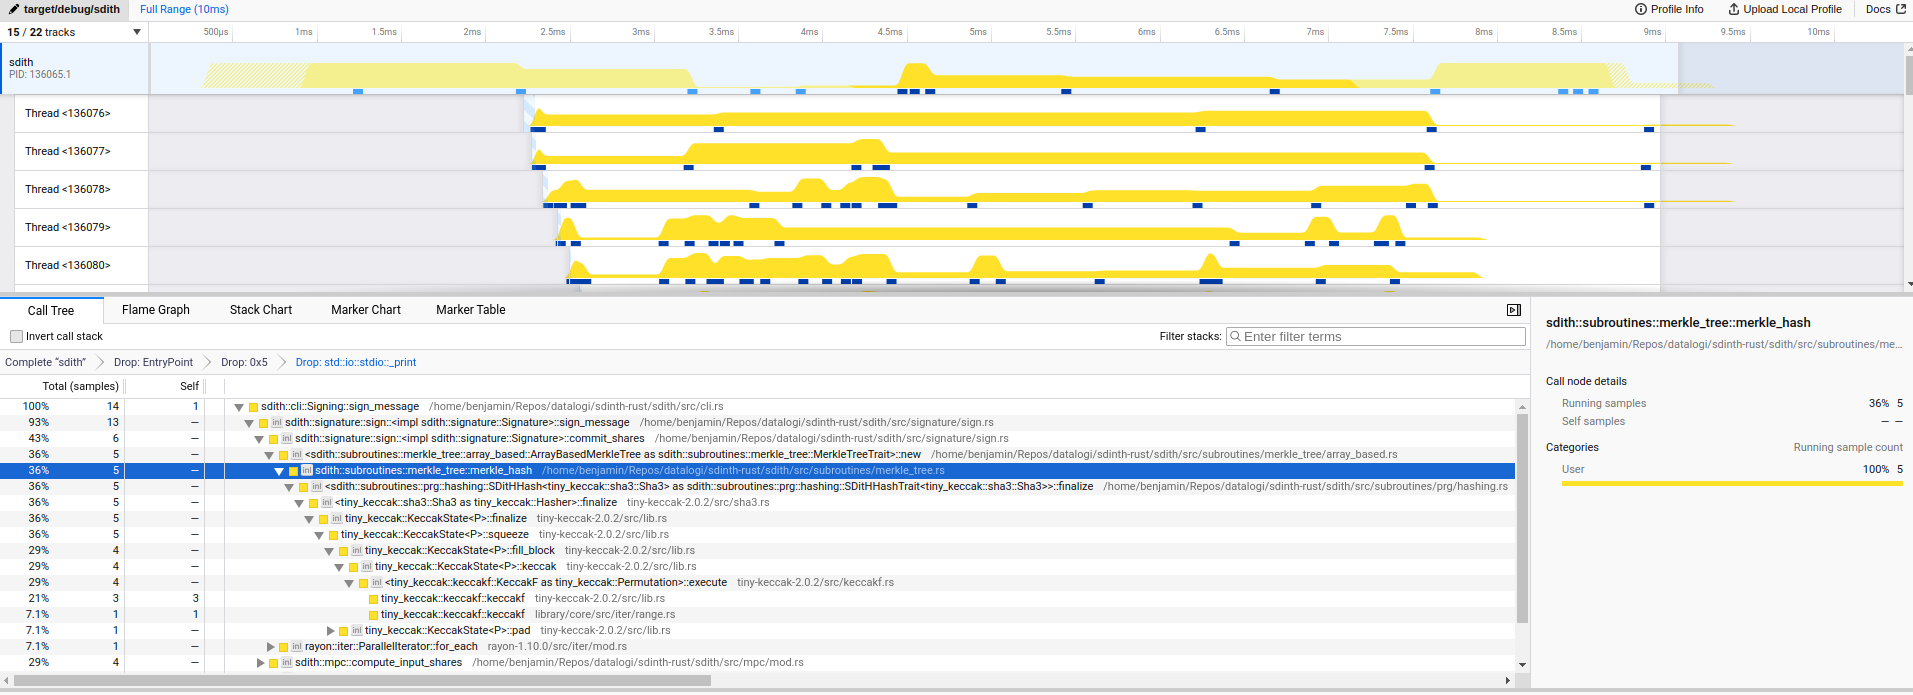
\includegraphics[width=\textwidth]{images/samply.png}
  \caption{Samply Profiler HTML Output}
  \label{fig:samply}
\end{figure}


\subsection{Build Configuration}

Rust has a number of configurations that you can apply to the compiler when building a project. These are easily configured using \textit{profiles} in the \texttt{Cargo.toml} file. We configured our optimised release profile as follows:

\begin{minted}{toml}
  [profile.release]
  strip = "debuginfo"
  codegen-units = 1  
  lto = "fat"        
  opt-level = 3      
  panic = "abort"
\end{minted}

The release profile was configured to maximize optimization during the compilation process. Specifically, the following settings were applied:

\begin{itemize}
  \item \mintinline{toml}{strip = "debuginfo"}: This strips debug information from the binary, reducing its size and improving performance.

  \item \mintinline{toml}{codegen-units = 1}: This disables parallel code compilation, resulting in slower compilation times. However, it often provides increased runtime performance and reduces the binary size by allowing the compiler to optimize more effectively.

  \item \mintinline{toml}{lto = "fat"}: This enables ``fat'' Link Time Optimization (LTO), which attempts to optimize across all crates within the dependency graph, enhancing overall performance by analyzing and optimizing the entire codebase.

  \item \mintinline{toml}{opt-level = 3/"z"}: This applies the highest level of performance optimizations offered by the compiler, enabling aggressive optimizations for runtime efficiency. To test the difference between optimising for binary size and performance, we ran the \textit{release} profile with both level 3 and \mintinline{toml}{"z"}, which optimises for binary size as opposed to performance.

  \item \mintinline{toml}{panic = "abort"}: This setting ensures that the program aborts immediately on a panic, without performing unwinding. If unwinding (e.g., via the \rust{catch_unwind} macro) is not required, setting \texttt{panic} to \texttt{"abort"} reduces binary size and often provides a slight performance boost.
\end{itemize}

\subsubsection{Inlining}
A subtle but effective way to improve performance is to inline functions that are called many times, this removes the overhead of the function call. The Rust compiler will automatically inline functions if they are small enough. But there are some cases where this is not enough and the compiler does not inline. In this case we can use the \texttt{inline} attribute to force the compiler to inline a function. Cachegrind is a good profiling tool to check if a function is inlined by the compiler.
\todo{Maybe revise this}

\subsubsection{Parallelisation}
A common optimization technique in modern programming is to leverage the multi-core architecture of modern CPUs by employing \textit{parallelization} or \textit{multi-threading}. This approach allows programs to execute multiple tasks concurrently, significantly improving performance for computationally intensive operations.

In many programming languages, multi-threading support is either limited or not guaranteed, often requiring developers to rely on external libraries or frameworks. However, Rust provides robust and native support for \textit{thread-safe} parallelization. With Rust's ownership system and built-in concurrency primitives, developers can write highly performant parallel code while minimizing risks of common concurrency issues such as data races or deadlocks.

The \textit{rayon}~\cite{rayon} package implements easy-to-use and lightweight data-parallelisation through their parallel iterators
\begin{minted}{rust}
  use rayon::prelude::*;
  fn sum_of_squares(input: &[i32]) -> i32 {
      input.par_iter() // <-- just change that!
          .map(|&i| i * i)
          .sum()
  }
\end{minted}

\subsubsection{Single Instruction Multiple Data (SIMD)}
Single Instruction Multiple Data or SIMD for short, is a way to better utilize a CPU when dealing with data in the form of Vectors. It is a way for the CPU to do a single instruction but on multiple data points at the same time by splitting the data into chunks that fit into a single register. This can greatly improve performance when dealing with large amounts of data. Rust has support for SIMD through the \texttt{std::simd} module. This module provides access to a portable abstraction for SIMD operations that is not bound to any particular hardware architecture.

A simple example could be adding two vectors together:
\begin{minted}{rust}
fn simple_vector_addition() -> [f32; 4] {
    let mut x = [1.0, 2.0, 3.0, 4.0];
    let y = [4.0, 3.0, 2.0, 1.0];
    for i in 0..4 {
        x[i] += y[i];
    }
    x
}

\end{minted}

Instead of looping through the data we can use SIMD to do the operation in one go:

\begin{minted}{rust}
fn simple_simd_vector_addition() -> [f32; 4] {
    // create SIMD vectors
    let x: f32x4 = f32x4::from_array([1.0, 2.0, 3.0, 4.0]);
    let y: f32x4 = f32x4::from_array([4.0, 3.0, 2.0, 1.0]);

    // SIMD operation
    let z = x + y; // z = [5.0, 5.0, 5.0, 5.0]
    z.to_array() 
}
\end{minted}

\chapter{Specification}\label{ch:spec}

\todo{Should we remove "we's" and use something that underlines that we are not the authors or designers? We could also have a pre-emptive disclaimer}

The SD-in-the-Head protocol is founded on the computational hardness of the Syndrome Decoding (SD) problem for random linear codes over a finite field, as described in \autoref{sec:syndrome}. To recall, the problem is formally stated:
\begin{quote}
  Given a parity-check matrix $H \in \mathbb{F}_q^{(m-k) \times m}$ in standard form and a syndrome $y \in \mathbb{F}_q^{m-k}$, the challenge is to find a vector $x \in \mathbb{F}_q^m$ such that $Hx = y$ and $wt(x) \leq w$, where $wt(x)$ denotes the Hamming weight of $x$. This can be expressed as:
  \begin{align*}
    y = Hx = H'x_a + x_b, \quad \text{where } H' \in \mathbb{F}_q^{(m-k) \times k},
  \end{align*}
  with $x = (x_a \mid x_b)$ denoting the concatenation of subvectors $x_a$ and $x_b$.
\end{quote}

The SD-in-the-Head protocol establishes a signature scheme by demonstrating the correctness of a public SD instance $(H, y)$ using a secret witness derived from $x$. Its construction unfolds in three main steps:
\begin{enumerate}
  \item \textbf{Defining an MPC protocol:} Define a multi-party computation (MPC) protocol that enables $N$ parties to collaboratively verify the correctness of the public SD instance $(H, y)$ using a private witness $x$.
  \item \textbf{Transforming into a ZK-POK:} Convert the MPC protocol into a zero-knowledge proof of knowledge (ZK-POK) through the MPC-in-the-Head (MPCitH) framework, detailed in \autoref{sec:mpcinth}.
  \item \textbf{Deriving a signature scheme:} Adapt the ZKP into a digital signature scheme using the Fiat-Shamir transformation, as described in \autoref{sec:fiatshamir}.
\end{enumerate}

The construction is highly modular, allowing flexibility and adaptability, as you can tweak the SD instance, the MPC protocol, the MPCitH and Fiat-Shamir transformations. The authors propose two distinct protocol variants: the \textit{hypercube} variant and the \textit{threshold} variant. For this work, we focus on the \textit{threshold} variant~\cite{aguilarsyndrome11,feneuil2023threshold,feneuil2023threshold2}, as it offers significant performance enhancements compared to both the initial protocol~\cite{feneuil2022syndrome} and the \textit{hypercube} variant~\cite{aguilarsyndrome11,aguilar2023return,feneuil2023threshold2}, albeit at the cost of slightly larger signature sizes.

This chapter presents a comprehensive specification of the SD-in-the-Head Signature Scheme in the Threshold variant. The construction is based on the SD-in-the-Head MPC protocol in \autoref{sec:sdith-mpc}, its transformation into ZK-POK using MPCitH (described in \autoref{sec:sdith-zkpok}) and finally transformation into a signature scheme in \autoref{sec:sdith-signature}. Additionally, we describe optimizations applied to the protocol, such as avoiding interpolation and utilizing the $d$-split variant of the SD instance. A detailed table summarizing the protocol parameters and security assumptions is provided in \autoref{tab:sdith-protocol-parameters}.

\begin{table}[]
  \begin{tabular}{p{0.12\textwidth}p{0.78\textwidth}}
    \hline
    \multicolumn{2}{l}{\textbf{Syndrome Decoding Parameters}}                                                                             \\
    $q$                          & Size of the SD base field.                                                                             \\
    $m$                          & Code length.                                                                                           \\
    $k$                          & Vector dimension.                                                                                      \\
    $w$                          & Hamming weight bound.                                                                                  \\
    $d$                          & Parameter of the $d$-splitting variant.                                                                \\ \hline

    \multicolumn{2}{l}{\textbf{Signature Parameters}}                                                                                     \\
    $\lambda$                    & Security parameter.                                                                                    \\
    $N$                          & Number of secret parties.                                                                              \\
    $\tau$                       & Number of repetitions.                                                                                 \\
    $t$                          & Number of random evaluation points.                                                                    \\ \hline

    \multicolumn{2}{l}{\textbf{Syndrome Decoding Instance}}                                                                               \\
    $H$                          & Parity-check matrix.                                                                                   \\
    $x$                          & Solution of the SD instance satisfying $wt(x) \leq w$.                                                 \\
    $y$                          & Syndrome computed as $y = Hx$.                                                                         \\
    $H'$                         & Random part of the parity-check matrix such that $H = (H' \mid I_{m-k})$.                              \\
    $(x_A, x_B)$                 & Two halves of the SD solution satisfying $y = H' x_A + x_B$.                                           \\ \hline

    \multicolumn{2}{l}{\textbf{Fields}}                                                                                                   \\
    $\mathbb{F}_q$               & Field with $q$ elements: base field of the SD instance.                                                \\
    $f_1, \ldots, f_q$           & Elements of $\mathbb{F}_q$.                                                                            \\
    $\mathbb{F}_{\text{points}}$ & Extension field of $\mathbb{F}_q$ (base field of the MPC elements $\alpha, \beta, v, r, \varepsilon$). \\
    $\eta$                       & Field extension such that $\mathbb{F}_{\text{points}} = \mathbb{F}_q^\eta$.                            \\ \hline

    \multicolumn{2}{l}{\textbf{Multi-Party Computation}}                                                                                  \\
    $S, Q, P$                    & Polynomials in $\mathbb{F}_q[X]$, witnesses for the syndrome decoding proof.                           \\
    $F$                          & Vanishing polynomial of the set $\{f_1, \ldots, f_m\} \subseteq \mathbb{F}_q$                          \\
    $a, b, c$                    & Beaver triple satisfying $a_k \cdot b_k = c_k$, $\forall k \in [1 : t]$.                               \\
    $\alpha, \beta, v$           & Broadcast values (coordinates in $\mathbb{F}_{\text{points}}$).                                        \\
    $i$                          & Index of a party in $[1 : N]$.                                                                         \\
    $\sh{v}$                     & Sharing of a value $v$.                                                                                \\
    $p$                          & False positive probability of the MPC protocol.                                                        \\
    $\ell$                       & Privacy threshold (number of open parties).                                                            \\
    $I$                          & Set of open parties $(I \subseteq [1 : N], |I| = \ell)$.                                               \\
  \end{tabular}
  \caption{SDitH protocol parameters overview~\cite[Table 1]{aguilarsyndrome11}.}\label{tab:sdith-protocol-parameters}
\end{table}

\section{The MPC Protocol}\label{sec:sdith-mpc}

The SD-in-the-Head protocol builds upon the \textit{Multi-Party Computation in the Head} (MPCitH) framework. As a first step, we describe the underlying MPC protocol, which is used to verify the polynomial relation of the SD instance as detailed in \autoref{sec:polynomial_representation}:
\begin{align*}
  S \cdot Q = P \cdot F, \quad \text{where } S, Q, P, F \in \mathbb{F}_q[X].
\end{align*}

The foundations for secret sharing and multi-party computation (MPC) are presented in \autoref{sec:additive-sss} and \autoref{sec:mpc}, respectively. The SD-in-the-Head MPC protocol is constructed using the sacrificing protocol introduced by Baum and Nof~\cite{baum2020concretely}, as detailed in \cref{sec:mpc_sacrificing}.

Recall, that instead of sharing $x_A$, we tweak the SD instance to share $s_A$ instead allowing us to skip interpolation detailed in \autoref{sec:syndrome-avoid-interpolation}

\begin{protocol}[SD-in-the-Head MPC protocol]\label{def:sdith-mpc}
  Assume the existence of a \textit{random oracle} $R$ and a $(N-2)$-\textit{private secret sharing scheme}. Given a public SD instance $(H, y)$, and the private sharings for each party $(\sh{s_A}, \sh{P}, \sh{Q})$, as well as $t$ sharings of random Beaver triples $\sh{a}, \sh{b}, \sh{c}$, the protocol proceeds as follows:
  \begin{enumerate}
    \item Sample $r^j, \varepsilon^j \in_R \mathbb{F}_{q^4}^t$ uniformly at random.
    \item For each party $P_i \in [1 : N]$:
          \begin{enumerate}
            \item Set $\sh{s_B} = y - H' \sh{s_A}$ and $\sh{S} = (\sh{s_A} \mid \sh{s_B})$.\label{step:sdith-mpc-lagrange-interpolation}
            \item Locally evaluate $\sh{S(r^j)}$, $\sh{Q(r^j)}$, and $\sh{F \cdot P(r^j)}$ for all $r^j \in \mathbb{F}_{q^4}^t$.
          \end{enumerate}
    \item For all $j \in [t]$, parties verify $\sh{S(r^j)} \cdot \sh{Q(r^j)} = \sh{P \cdot F(r^j)}$ by sacrificing \\$(\sh{a^j}, \sh{b^j}, \sh{c^j})$:
          \begin{enumerate}[topsep=0pt]
            \item Parties locally compute $\sh{\alpha^j}  = \varepsilon^j \cdot \sh{Q(r^j)} + \sh{a^j}$ and $ \sh{\beta^j}  = \sh{S(r^j)} + \sh{b^j}$.
            \item Parties broadcast $\sh{\alpha^j}$ and $\sh{\beta^j}$ to publicly recompute $\alpha^j$ and $\beta^j$.
            \item Parties locally compute:
                  \begin{align*}
                    \sh{v^j} & = \varepsilon^j \cdot \sh{F \cdot P(r^j)} - \sh{c^j} + \alpha^j \cdot \sh{b^j} + \beta^j \cdot \sh{a^j} - \alpha^j \cdot \beta^j.
                  \end{align*}
            \item Parties broadcast $\sh{v^j}$ to publicly recompute $v^j$.
            \item Parties output \texttt{Accept} if $v^j = 0$, and \texttt{Reject} otherwise.
          \end{enumerate}
  \end{enumerate}
\end{protocol}

To analyze the security of the protocol, we denote $p$ as the false positive probability. $p$ quantifies the likelihood that the MPC protocol incorrectly accepts an invalid instance~\cite{feneuil2022syndrome,aguilarsyndrome11}.

\begin{lemma}[False positive probability $p$ of \autoref{def:sdith-mpc}]\label{lem:sdith-mpc-soundness}
  Let $x_A = \texttt{open}(\sh{x_A})$. If $x_A$ corresponds to a valid SD instance $(H', y)$ and if all sharings are correctly generated. Then \autoref{def:sdith-mpc} always outputs \texttt{Accept}.
  Otherwise, the probability of a false positive is bounded by
  \begin{align*}
    p = \sum_{i=0}^t \frac{\max_{j \leq m + w -1} \{ \binom{j}{i} \binom{\Delta - j}{t-i} \}}{\binom{\Delta}{t}} \cdot \left(\frac{1}{\Delta}\right)^{t-i}
  \end{align*} over the randomness $r$ and $\varepsilon$ and $\Delta = |\mathbb{F}_{q^4}|$.
\end{lemma}

\section{The Threshold Signature Protocol}\label{sec:sdith-signature}

The initial protocol for the SD-in-the-Head signature scheme is seen in~\cite[Figure 1]{aguilarsyndrome11} and was first introduced in~\cite[Figure 1, p19]{feneuil2022syndrome}.

\subsubsection{Threshold variant}\label{sub:sdith-threshold-sss}

The threshold variant of the MPC protocol (\autoref{def:sdith-mpc}) is obtained by incorporating \textit{Shamir's Secret Sharing Scheme} (SSSS), as described in \autoref{sub:shamir}. By replacing the additive secret sharing scheme with Shamir's polynomial-based scheme, the protocol is extended into a $(\ell, N)$-threshold MPC protocol, where any $\ell$ out of $N$ parties can reconstruct the secret, while $\ell-1$ parties gain no information about the secret.

\begin{theorem}[Linear functions of \autoref{def:sdith-mpc}]\label{thm:sdith-mpc-linear}
  By the definition of the MPC protocol \autoref{def:sdith-mpc}, there exist linear functions
  \begin{align}
    \varphi^1_{r,\varepsilon}                 & : (s_A, P, Q, a, b, c) \mapsto (\alpha, \beta), \\
    \varphi^2_{r, \varepsilon, \alpha, \beta} & : (s_A, P, Q, a, b, c) \mapsto v,
  \end{align}
  such that each party locally computes $\varphi^1$ and $\varphi^2$ on the input shares $\sh{s_A}_i, \sh{P}_i, \sh{Q}_i, \sh{a}_i, \sh{b}_i, \sh{c}_i$, and randomness $r, \varepsilon$ producing $\sh{\alpha}_i, \sh{\beta}_i, \sh{v}_i$ as valid sharings of $\alpha, \beta, v$.
\end{theorem}

The authors suggest a tweak to the MPC input generation in the following way: Define the \texttt{input\_plain} as the tuple containing the MPC inputs:
\begin{align*}
  \texttt{input\_plain} = (s_A, P, Q, a, b, c)
\end{align*}

Next, compute $\ell$ uniformly random coefficients $\texttt{input\_coef} \in \mathbb{F}_q^{|\texttt{input\_plain}|}$ and compute the i'th sharing of the \texttt{input\_plain}:
\begin{align}\label{equation:input_sharing}
  \sh{\texttt{input\_plain}}_i = \texttt{input\_plain} + \sum_{j=1}^\ell f_i^j \cdot \texttt{input\_coef}_j
\end{align}
Where the $f_1,\dots,f_N$ denotes $N$ non-zero elements from the field $\mathbb{F}_q$.
The MPC computation is then performed directly on the \texttt{input\_plain} and its $\ell$ coefficients from the SSSS:
\begin{align*}
  \texttt{input\_plain}     & \stackrel{\varphi^1, \varphi^2}{\longrightarrow} \texttt{broad\_plain}     \\
  \texttt{input\_coef}_1    & \stackrel{\varphi^1, \varphi^2}{\longrightarrow} \texttt{broad\_coef}_1    \\
                            & \vdots                                                                     \\
  \texttt{input\_coef}_\ell & \stackrel{\varphi^1, \varphi^2}{\longrightarrow} \texttt{broad\_coef}_\ell
\end{align*}

Due to the linearity of the MPC computation, the output shares can be reconstructed by running the sharing protocol on the broadcast shares:
\begin{align}\label{equation:input_sharing_reverse}
  (\sh{\alpha}_i, \sh{\beta}_i, \sh{v}_i) = \texttt{broad\_plain} + \sum_{j=1}^\ell f_i^j \cdot \texttt{broad\_coef}_j
\end{align}

\subsubsection{PK setup}
The nature of an SD instance allows the protocol to seamlessly transform into a \textit{public-key signature scheme}. Here, the pair $(H, y)$ acts as the public key, while the solution to the SD instance $x$ serves as the private key. The keys is then expanded to $(H', y), (s_A, P, Q)$ following the transformations detailed in \autoref{sec:syndrome}. Furthermore, the public key can be optimised for communication by instead sampling $H'$ from a seed $sd_H$ making the secret key $(sd_H, y)$.

\subsubsection{ZK-POK protocol}
First, the MPC protocol (\autoref{def:sdith-mpc}) is transformed into a ZK-POK) using the Threshold MPCitH protocols described by~\cite{feneuil2023threshold,feneuil2023threshold2}. This transformation in full lies outside the scope of this report and is deferred to the appendix in \autoref{sec:sdith-zkpok}. Here we leave a short overview of the transformation~\cite{aguilarsyndrome11}.

\begin{protocol}[SD-in-the-Head ZK-POK protocol]
  \label{pro:sdith-zkpok}
  For a $(\ell + 1, N)$-threshold MPC protocol
  \begin{enumerate}[parsep=0pt, itemsep=0pt, topsep=0pt]
    \item The prover generates the input sharings and commits to the parties' shares in $h_1$
    \item The verifier challenges the prover with the randomness \(r, \varepsilon\) for the MPC protocol. This is called the \textit{MPC challenge}.
    \item The prover executes the MPC protocol (in their head) and sends the broadcast values to the verifier in $h_2$
    \item The verifier challenges the prover to open all the parties in \(I \subset [N]\) for $|I| = \ell$. This is called the \textit{viewchallenge}.
    \item The prover reveals the input shares of all the parties in \(I\).
    \item The verifier verifies the consistency of the MPC computation for the revealed parties.
  \end{enumerate}
\end{protocol}

The zero-knowledge property of the protocol is guaranteed by the fact that the verifier only receives $\ell$ shares from an $\ell + 1$-private secret-sharing scheme (SSS). 
The soundness of the ZK-POK protocol relies on the binding property of the commitment scheme and the prover's inability to simulate multiple inconsistent views of the MPC protocol. By incorporating hash consistency checks and commitment verification, the ZK-POK protocol ensures that a cheating prover cannot deviate significantly from the behavior expected in an honest execution.

As outlined in~\cite{feneuil2023threshold}, the general ZK-POK (without threshold) soundness error is defined as:
\begin{align*}
  \epsilon = \frac{1}{N} + p \cdot \left(1 - \frac{1}{N}\right).
\end{align*}
By applying the threshold-based approach, the soundness error is modified and becomes:
\begin{lemma}[Soundness of \autoref{pro:sdith-zkpok}]
  The soundness error $\epsilon$ is given by:
  \begin{align*}
    \epsilon = \frac{1}{\binom{N}{\ell}} + p \cdot \frac{\ell \cdot (N - \ell)}{\ell + 1},
  \end{align*}
  where $p$ represents the false positive probability of the MPC protocol, $N$ is the total number of parties, and $\ell$ is the threshold parameter~\cite{feneuil2023threshold}.
\end{lemma}
We can see that the threshold-based approach introduces a slight degradation in the soundness of the protocol. This comes from the fact that we now require less views to be validated, which in turn increases the probability of a false positive.
To mitigate this, \textit{parallel repetition} is employed to strengthen the soundness signature protocol. Specifically, the SD-in-the-Head protocol repeats the underlying ZK-POK protocol $\tau$ times, where:
\begin{align*}
  \tau = \left\lceil \log_2\left(\frac{1}{\epsilon}\right) \cdot \lambda \right\rceil,
\end{align*}
with $\lambda$ as the security parameter and $2^{-\lambda}$ as the target soundness error~\cite{aguilarsyndrome11}. This parallel repetition reduces the overall soundness error exponentially with the number of repetitions, achieving a negligible error probability in practice.

To accommodate the repetitions, the authors incorporate a slight modification inspired by the Limbo proof system~\cite{delpech2021limbo}. Specifically, we reuse the same MPC challenges $r$ and $\varepsilon$, as well as the Beaver triples, across all $\tau$ repetitions. This tweak allows us to modify the MPC computation input so that \textit{plain bradcast} value only needs to be computed once.

\subsubsection{Fiat-Shamir transform}
Next, we apply the \textit{Fiat-Shamir heuristic} -- detailed in \autoref{sec:fiatshamir} -- to transform the challenges of the ZK-POK protocol into a non-interactive form. This transformation is achieved by having the prover derive the challenges for MPC randomness and opening challenge directly from the commitments of the MPC inputs and the outputs of the MPC computation in the hashes $h_1, h_2$ computed from secure hash functions~\autoref{sec:prelim_hash}.
\begin{align}
  h_n = \texttt{Hash}_n(d) \rightarrow \texttt{Hash}(n || d)\label{eq:fiatshamirhash}
\end{align}

Additionally, we incorporate the message into the second hash, enabling the pre-computation of the first part of the signature independently of the message. This optimization enhances efficiency by allowing some computations to be performed beforehand.

Finally, we introduce a $\texttt{salt} \in \{0,1\}^{2\lambda}$, which serves as pseudo-randomness for commitments and seed generation. The use of a $\texttt{salt}$ ensures that the protocol remains secure and avoids reliance on externally provided randomness.

\subsubsection{Optimizing Signature Size and Verification}
In the original SD-in-the-Head protocol~\cite[Figure 1]{aguilarsyndrome11} -- without threshold SSS -- the signature includes both hashes $h_1, h_2$ and all input shares in $I$, where $|I| = N - 1$. 
To verify the signature, the verifier recomputes the commitments for each share in $I$, and along with the last missing commitment $\texttt{com}_i$ for $i \notin I$, reconstructs $h_1$. The verifier then executes the MPC protocol for the opened shares and recomputes $h_2$ from the resulting output shares.

\begin{theorem}[Sharing Redundancy of Shamir's Secret Sharing Scheme]
  The full set of broadcast shares $\sh{\alpha}_i, \sh{\beta}_i, \sh{v}_i$ for $i \in N$ can be deduced from $\ell + 1$ broadcast shares. That is, the full sharing forms a Reed-Solomon code word.
\end{theorem}

\noindent
For the threshold variant, however, we can optimize this process by selecting a predefined set
\begin{align*}
  \mathcal{E} = \{\sh{\alpha}_i, \sh{\beta}_i, \sh{v}_i\}_{i \in E},
\end{align*}
where $E \subseteq N$ and $|E| = \ell + 1$. We then set $h_2 = \texttt{Hash}_2(\mathcal{E})$. In this case, the signature includes the input shares $\{\sh{\alpha}_i, \sh{\beta}_i, \sh{v}_i\}_{i \in I}$, plus a single broadcast share, allowing the verifier to recompute $h_2$. However, this approach requires the verifier to interpolate the sharing coefficients
\begin{align}
  \texttt{broad\_plain}, \texttt{broad\_coef}_1, \dots, \texttt{broad\_coef}_\ell.\label{eq:mpc_shamir_coeffs}
\end{align}
To avoid this interpolation, we note that $\mathcal{E}$ is fully determined by the coefficients. Therefore, we can instead use these as the input of $h_2$, enabling the signer to bypass the computation of $\mathcal{E}$. Furthermore, the signature can include \autoref{eq:mpc_shamir_coeffs} instead of $h_2$. This allows the verifier to compute $h_2$ and evaluate $\{\sh{\alpha}_i, \sh{\beta}_i, \sh{v}_i\}_{i \in I}$ directly, avoiding the need for interpolation.

Following from \autoref{thm:sdith-mpc-linear}, for every party $i$, there exists a direct linear relationship between the Beaver triple shares $\sh{a}_i, \sh{b}_i, \sh{c}_i$ and the broadcast shares $\sh{\alpha}_i, \sh{\beta}_i, \sh{v}_i$. This observation enables the removal of Beaver triples within the signature. Instead, the verifier can compute these triples directly using the shares of the witness, $(\sh{s_A}_i, \sh{P}_i, \sh{Q}_i)$, along with the broadcast shares $(\sh{\alpha}_i, \sh{\beta}_i, \sh{v}_i)$ for $i \in I$. We denote a function \textit{TruncateBeaver}
\begin{align}
  \text{TruncateBeaver} : \sh{\texttt{input}}_i = (\sh{s_A}_i, \sh{P}_i, \sh{Q}_i, \sh{a}_i, \sh{b}_i, \sh{c}_i) \mapsto (\sh{s_A}_i, \sh{P}_i, \sh{Q}_i) = \sh{\texttt{wit}}_i\label{eq:truncate_beaver}
\end{align}
This process is referred to as \textit{reverse MPC computation}

\begin{theorem}[Reverse MPC computation]\label{thm:mpc_reverse}
  For a MPC protocol \autoref{thm:sdith-mpc-linear} we have a reverse MPC computation with two functions
  \begin{align}
    \phi^1_{r,\varepsilon}        & : (s_A, P, Q, \alpha, \beta, v) \mapsto (a, b), \\
    \phi^2_{r, \varepsilon, a, b} & : (s_A, P, Q, \alpha, \beta, v) \mapsto c,
  \end{align}

  We have that for any $(a,b,c) \stackrel{\phi^1, \phi^2}{\longleftarrow} (s_A, P, Q, \alpha, \beta, v, r, \varepsilon)$, then
  \begin{align*}
    (s_A, P, Q, a, b, c, r, \varepsilon) \stackrel{\varphi^1, \varphi^2}{\longrightarrow} (\alpha, \beta, v)
  \end{align*}
\end{theorem}

To formalize the approach, we introduce the following notations:

Denote $Q'$ as the witness polynomial $Q$ with its leading coefficient removed. Additionally, let $\sh{Q^0}$ represent the polynomial with a leading coefficient of $0$, and $\sh{Q^1}$ the polynomial with a leading coefficient of $1$.

Define two reconstructions of $S$ as:
\begin{align*}
  S_1 & = (s_A, y - H \cdot s_A), \\
  S_0 & = (s_A, H \cdot s_A).
\end{align*}

These two updates enable the reverse MPC computation by ensuring that the constant parts of the affine functions are introduced for one party and therefore not removed during the reverse MPC computation.

Therefore, we include an input parameter \texttt{with\_offset} in the MPC protocol \autoref{def:sdith-mpc}, denoted $\varphi^1_{\texttt{with\_offset}}$. This parameter determines whether $S_{\texttt{with\_offset}}, Q_{\texttt{with\_offset}}$ is used. Similarly, $\varphi^2_{\texttt{with\_offset}}$ indicates whether the constant derived from the plain outputs, $-\alpha \cdot \beta$, is added to $v$.

The same applies to $\phi^1$ and $\phi^2$ for the reverse MPC computation. For further clarity, a \textit{toy example} illustrating the reverse MPC computation is provided in \autoref{app:toy_example}.

\subsubsection{The protocols}
We introduce the signing and verification protocols in \autoref{def:sdith-sign} and \autoref{def:sdith-verify}, respectively.

\begin{protocol}[SD-in-the-Head Signing Protocol]\label{def:sdith-sign}
  \setlength{\parindent}{0pt}
  \setlength{\parskip}{5pt}
  \titlespacing*{\paragraph}{0pt}{1pt}{1em}
  Given a public key (SD instance) $pk = (H, y)$, secret key (SD solution) $sk = (s_A, Q, P)$, message $m \in \{0,1\}^*$ and security parameters $\lambda, \tau$

  \paragraph{Assumptions} 

  \begin{itemize}[itemsep=0pt, topsep=0pt, parsep=0pt]
    \item $(\ell + 1, N)$-threshold MPC protocol $\varphi^1, \varphi^2$ (\autoref{def:sdith-mpc}, \autoref{sec:mpc}), \autoref{equation:input_sharing}
    \item Merkle Tree Commitment Scheme: \texttt{MerkleTree} and \texttt{MerkleAuthPath} (\autoref{sub:merkle_tree_prelim})
    \item Collision Resistant hash functions $\texttt{Hash}_n$ (\autoref{eq:fiatshamirhash})
    \item Random oracle $\texttt{PRG}$ (\autoref{sec:prelim_hash})
    \item Extendable output hash function \texttt{XOF} (\autoref{sec:xof})
  \end{itemize}

  \paragraph{Setup} Initialise entropy

  \begin{enumerate}[itemsep=0pt, topsep=0pt, parsep=0pt]
    \item Sample a random salt: $\texttt{salt} \leftarrow \{0, 1\}^{2\lambda}$.
    \item Sample a root seed: $sd \leftarrow \{0, 1\}^{\lambda}$.
    \item Initialise \texttt{XOF} from $sd$, \texttt{salt}
  \end{enumerate}
  \paragraph{Phase 1} Prepare the MPCitH inputs.

  \begin{enumerate}[itemsep=0pt, topsep=0pt, parsep=0pt]
    \item Compute Beaver triples $\mathcal{B} = a^{j}, b^{j}, c^{j}$ for all $j \in t$ and construct $\texttt{input\_plain} = (sk, \mathcal{B})$
    \item For each iteration $e \in [\tau]$
          \begin{enumerate}[itemsep=0pt, topsep=2pt, parsep=0pt]
            \item compute $\texttt{input\_coef}_j^e \leftarrow \texttt{XOF}$ for each $j \in \ell$
            \item compute input shares for $i \in [N]$
                  \begin{align*}
                    \sh{\texttt{input\_plain}}_i^e =
                    \begin{cases}
                      \texttt{input\_coef}^e_{\ell}                                                   & \quad i = 1 \\
                      \texttt{input\_plain} + \sum_{j=1}^\ell f_i^j \cdot \texttt{input\_coef}_j^e & \quad i > 1
                    \end{cases}
                  \end{align*}
            \item compute commitments for $i \in [N]$
                  \begin{align*}
                    \texttt{com}_i^{e} := \texttt{Hash}_0(\texttt{salt}, e, i, \sh{\texttt{input\_plain}}_i^e)
                  \end{align*}
            \item compute the Merkle commitment
                  \begin{align*}
                    \texttt{root}^{e} = \texttt{MerkleTree}(\texttt{com}_1^{e}, \ldots, \texttt{com}_N^{e})
                  \end{align*}
          \end{enumerate}
  \end{enumerate}

  \paragraph{Phase 2} Compute first challenge (\textit{MPC challenge})
  \begin{enumerate}[itemsep=0pt, topsep=0pt, parsep=0pt]
    \item Compute the first hash
          \begin{align*}
            h_1 = \texttt{Hash}_1(pk, \texttt{salt}, \texttt{root}^{1}, \ldots, \texttt{root}^{\tau})
          \end{align*}
    \item Generate first challenge (MPC randomness)
          \begin{align*}
            r, \varepsilon \leftarrow \texttt{PRG}(h_1)
          \end{align*}
  \end{enumerate}

  \paragraph{Phase 3} Simulation of the MPC Protocol.
  \begin{enumerate}[itemsep=0pt, topsep=0pt, parsep=0pt]
    \item Compute plain broadcast $\texttt{broad\_plain} \stackrel{\varphi^1_1}{\longleftarrow} \texttt{input\_plain}, r, \varepsilon$\footnote{$\varphi^2$ is skipped as $v = 0$ for an honest execution.}
    \item For $e \in [\tau]$, compute broadcast shares
          \begin{align*}
            \texttt{broad\_coef}_j^e \stackrel{\varphi^1_0, \varphi^2_0}{\longleftarrow} \texttt{input\_coef}_j^e, r, \varepsilon \quad \text{for each } j \in \ell
          \end{align*}
  \end{enumerate}

  \paragraph{Phase 4} Compute second challenge (\textit{View opening challenge})
  \begin{enumerate}[itemsep=0pt, topsep=0pt, parsep=0pt]
    \item Compute the second hash
          \begin{align*}
            h_2 = \texttt{Hash}_2(m, \texttt{salt}, h_1, \texttt{broad\_plain}, \{\texttt{broad\_coef}^e_1, \dots, \texttt{broad\_coef}^e_\ell\}_{e=1}^\tau)
          \end{align*}
    \item Compute the second challenge $I \subset [N] \leftarrow \texttt{PRG}(h_2)$ for $|I| = \ell$
  \end{enumerate}

  \paragraph{Phase 5} Building of the signature output the signature $\sigma$ for $e \in [\tau]$ and $i \in I$
  \begin{enumerate}[itemsep=0pt, topsep=0pt, parsep=0pt]
    \item Compute authentication paths
          \begin{align*}
            \texttt{auth}^e = \texttt{MerkleAuthPath}(\{\texttt{com}^e_i\}_{i \in I})
          \end{align*}
    \item Compute witness shares
          \begin{align*}
            \sh{\texttt{wit}}_i^e = \text{TruncateBeaver}(\texttt{input}^e_i)
          \end{align*}
    \item Build the signature
          \begin{align*}
            \sigma = & \ (\ m\ |\ \texttt{salt}\ |\ h_1                                  \\
                     & \ |\ \texttt{broad\_plain}                                        \\
                     & \ |\ \texttt{broad\_coef}^e_1, \dots, \texttt{broad\_coef}^e_\ell \\
                     & \ |\ \texttt{auth}^e                                              \\
                     & \ |\ \sh{\texttt{wit}}_i^e                                        \\
                     & \ |\ I\ )
          \end{align*}
  \end{enumerate}
\end{protocol}

\begin{protocol}[SD-in-the-Head Verification Protocol]\label{def:sdith-verify}
  \setlength{\parindent}{0pt}
  \setlength{\parskip}{5pt}
  \titlespacing*{\paragraph}{0pt}{1pt}{1em}
  Given a public SD instance $pk = (H, y)$, security parameters $\lambda, \tau$, and a signature
  \begin{align*}
    \sigma = & \ (\ m\ |\ \texttt{salt}\ |\ h_1                                  \\
             & \ |\ \texttt{broad\_plain}                                        \\
             & \ |\ \texttt{broad\_coef}^e_1, \dots, \texttt{broad\_coef}^e_\ell \\
             & \ |\ \texttt{auth}^e                                              \\
             & \ |\ \sh{\texttt{wit}}_i^e                                        \\
             & \ |\ I\ )
  \end{align*}

  \paragraph{Assumptions}
  \begin{enumerate}[itemsep=0pt, topsep=0pt, parsep=0pt]
    \item $(\ell + 1, N)$-threshold MPC protocol with reverse computation $\phi^1, \phi^2$ (\autoref{def:sdith-mpc}, \autoref{thm:mpc_reverse}, \autoref{sec:mpc}), \autoref{equation:input_sharing_reverse}
    \item Merkle Tree Commitment Scheme: \texttt{MerkleRootFromAuthPath} (\autoref{sub:merkle_tree_prelim})
    \item Collision resistant  hash functions $\texttt{Hash}_n$ (\autoref{eq:fiatshamirhash})
    \item Random oracle $\texttt{PRG}$ (\autoref{sec:prelim_hash})
    \item Extendable output hash function \texttt{XOF} (\autoref{sec:xof})
  \end{enumerate}

  \paragraph{Protocol} The protocol proceeds as follows for $e \in [\tau]$ and $i \in I$:
  \begin{enumerate}[itemsep=0pt, topsep=0pt, parsep=0pt]
    \item Recompute the first challenge $r, \varepsilon \leftarrow \texttt{PRG}(h_1)$
    \item Compute broadcast shares
          \begin{align*}
            \mathcal{B'}_i = \sh{\alpha^e}_i, \sh{\beta^e}_i, \sh{v^e}_i =
            \begin{cases}
              \texttt{broad\_coef}^e_\ell                                                     & \quad i = 1 \\
              \texttt{broad\_plain} + \sum_{j=1}^\ell f_i^j \cdot \texttt{broad\_coef}_j^e & \quad i > 1
            \end{cases}
          \end{align*}
    \item Recompute Beaver triples
          \begin{align*}
            \sh{a}_i, \sh{b}_i, \sh{c}_i \stackrel{\phi^1_{i > 1}, \phi^2_{i > 1}}{\longrightarrow} (pk, \texttt{broad\_plain}, \sh{\texttt{wit}}_i^e, \mathcal{B'}_i, r, \varepsilon)
          \end{align*}
          Set $\texttt{input}^e_i = (\texttt{wit}_i^e, \mathcal{B'}_i)$
    \item Recompute commitments
          \begin{align*}
            \texttt{com}^e_i = \texttt{Hash}_0(\texttt{salt}, e, i, \sh{\texttt{input}^e_i})
          \end{align*}
    \item Recompute Merkle tree roots
          \begin{align*}
            \texttt{root}^e = \texttt{MerkleAuthPath}(\texttt{auth}^e,\{\texttt{com}^e_i\}_{i \in I})
          \end{align*}
    \item Recompute $\tilde{h_1} = \texttt{Hash}_1(pk, \texttt{salt}, \texttt{root}^e, \ldots, \texttt{root}^{\tau})$
  \end{enumerate}

  Output \texttt{Accept} if and only if $h_1 \stackrel{?}{=} \tilde{h_1}$, and \texttt{Reject} otherwise.

\end{protocol}

\section{Security}

The security analysis of the SD-in-the-Head signature scheme is based on the proposed standardization requirements from the 2022 NIST call for proposals of non-lattice based signature schemes~\cite{nistcall}. Therefore, as a preliminary, we will describe the reasoning and requirements of the NIST standardization process.

With the development of new quantum algorithms and unknowns in the capacities of the future quantum computers, there remain large uncertainties in estimating the security of the algorithms. To combat these uncertainties, NIST proposed for the 2022 stadardization effort, to define the security of submissions in a range of five categories. Each, with an easy-to-analyze cryptographic primitive providing the lower bound for a variety of metrics deemed relevant to practical security.

\begin{definition}\label{def:nistsec}
  Any attack that breaks the relevant security definition must require computational resources comparable to or greater than those required for key search on a block cipher with a 128-bit (e.g. AES-128), 192-bit (e.g. AES-192) and 256-bit (e.g. AES-256) for categories \textbf{one}, \textbf{three} and \textbf{five} respectively.
\end{definition}

In terms of quantum security, the complexity and capability of quantum algorithms are measured in terms of quantum circuit size, i.e. the number of quantum gates in the quantum circuit. In order to estimate the quantum security of the signature protocols, circuit size can be compared to the resources required to break the security of \autoref{def:nistsec}.

\subsubsection{NIST Categories}

The SD-in-the-Head specification provides security parameters adhering to categories one, three and five. Therefore, according to the proposal by NIST, the SD-in-the-Head specification provides security metrics in terms of quantum circuit depth to optimal key recovery for AES-128, AES-192 and AES-256 for categories \textbf{one}, \textbf{three} and \textbf{five} respectively. These are estimated to be $2^{143}$, $2^{207}$ and $2^{272}$ classical gates~\cite{nistcall}.

\subsubsection{Signature Forgery Attack}

The SD-in-the-Head signature scheme ensures \textbf{E}xistential \textbf{U}nforgeability under \textbf{C}hosen \textbf{M}essage \textbf{A}ttack (EUF-CMA), a key security property evaluated by NIST~\cite{nistcall,aguilarsyndrome11}. In the EUF-CMA game, a challenger generates a key pair $(pk, sk)$ and provides $pk$ to the adversary, who can query a signing oracle for up to $2^{64}$ chosen messages $(m_1, \dots, m_r)$, receiving corresponding valid signatures $(\sigma_1, \dots, \sigma_r)$. The adversary wins if it produces a valid signature $(m^*, \sigma^*)$ for a message $m^*$ not queried to the signing oracle.

We analyze the generic forgery attack on Fiat-Shamir transformed signature protocols as described by~\cite{kales2020attack}. This attack seeks to minimize the effective cost of a forgery attempt. For the threshold-based SD-in-the-Head protocol, the adversary can choose between two strategies:
\begin{enumerate}
  \item \label{item:guessing-mpc-challenge} Guessing the unique MPC challenge.
  \item \label{item:guessing-view-challenge} Guessing the view-opening challenges for each of the $\tau$ executions.
\end{enumerate}

In strategy~\ref*{item:guessing-mpc-challenge}, the adversary attempts to exploit false positives in the MPC protocol. This is lower bounded by the cost of obtaining a false positive for one truncated input share (see \autoref{eq:truncate_beaver}) in one of the $\tau$ executions, where the share is encoded by a subset $I \subset [N]$:
\begin{align*}
  \frac{1}{1 - (1-p)^{\tau \cdot \binom{N}{\ell + 1}}}.
\end{align*}

Due to the tweak in MPC input generation detailed in \autoref{sub:sdith-threshold-sss}, the adversary cannot use invalid shares to reduce the cost in strategy~\ref*{item:guessing-view-challenge}, as any such inconsistency will be detected by the verifier. Thus, the cost of this strategy corresponds to plain guessing:
\begin{align*}
  \binom{N}{\ell}^\tau.
\end{align*}

Therefore, the total cost of a forgery attack is the maximum of the two strategies:
\begin{align}
  \max \left\{ \frac{1}{1 - (1-p)^{\tau \cdot \binom{N}{\ell + 1}}}, \binom{N}{\ell}^\tau \right\}\label{eq:forgery_attack_cost}
\end{align}

\subsubsection{$d$-split Syndrome Decoding Problem}

Categories three and five rely on a variant of the syndrome decoding problem, referred to as the \textit{$d$-split syndrome decoding problem}. This variant introduces the splitting parameter $d$, which partitions the witness $x$ into $d$ chunks:
\begin{align*}
  x & = x_1 \| \dots \| x_d \in \mathbb{F}_q^{m/d} \quad \text{wt}(x_j) = w/d
\end{align*}
In this formulation, the MPC protocol is executed $d$ times in parallel. Consequently, the polynomial relations $Q$, $P$, $S$, and $F$ are divided into $d$ corresponding polynomials, e.g.,
\begin{align*}
  \textbf{Q} & = Q_1, \dots, Q_d.
\end{align*}
Similarly, the Beaver triples $a$ and $b$ are adjusted for the $d$-split as follows:
\begin{align*}
  c_j & = \sum_{i=1}^d a_{i,j} \cdot b_{i,j}, \quad j \in [\tau].
\end{align*}

While the $d$-split variant introduces a slight reduction in security compared to the standard SD problem, this is mitigated by a small increase in the security parameters $m$, and $w$. The primary advantage of this variant lies in its flexibility, enabling improved performance trade-offs~\cite{aguilarsyndrome11}. The increase in parameters are given by
\begin{align}
  \varepsilon_1 \geq \frac{\binom{m/d}{w/d}}{\binom{m}{w}} \cdot \epsilon_d\label{eq:d_split_epsilon}
\end{align}
a proof of this can be found in~\cite[p27]{feneuil2022syndrome}

\subsubsection{Parameters for the SD-in-the-Head protocol}

The parameters for the SD-in-the-Head protocol are given in \autoref{tab:secparam} and \autoref{tab:hashparam} are given by \autoref{eq:forgery_attack_cost} and \autoref{eq:d_split_epsilon}

\begin{table}[ht]\label{tab:secparam}
  \centering
  \def\arraystretch{1.5}%  1 is the default, change whatever you need
  \begin{tabular}{cccccccccccccc}
    \specialrule{.1em}{.05em}{.05em}
    \multicolumn{2}{c}{\textbf{NIST security}} &      & \multicolumn{5}{c}{\textbf{SD parameters}} &     & \multicolumn{5}{c}{\textbf{MPCitH Parameters}}                                                             \\ \cline{1-2} \cline{4-8} \cline{10-14}
    Category                                   & Bits &                                            & $q$ & $m$                                            & $k$ & $w$ & $d$ &  & N   & $\ell$ & $\tau$ & $\eta$ & $t$ \\ \hline
    \textbf{I}                                 & 143  & \textit{}                                  & 256 & 242                                            & 126 & 87  & 1   &  & $q$ & 3      & 17     & 4      & 7   \\
    \textbf{III}                               & 207  &                                            & 256 & 376                                            & 220 & 114 & 2   &  & $q$ & 3      & 26     & 4      & 10  \\
    \textbf{V}                                 & 272  &                                            & 256 & 494                                            & 282 & 156 & 2   &  & $q$ & 3      & 34     & 4      & 13  \\ \specialrule{.1em}{.05em}{.05em}
  \end{tabular}
  \caption{Security parameters for the SDitH protocol for categories one, three and five~\cite{aguilarsyndrome11}.}
\end{table}

\begin{table}[ht]\label{tab:hashparam}
  \centering
  \def\arraystretch{1.5}%  1 is the default, change whatever you need
  \begin{tabular}{clll}
    \specialrule{.1em}{.05em}{.05em}
         & \multicolumn{1}{c}{\textbf{I}} & \multicolumn{1}{c}{\textbf{III}} & \multicolumn{1}{c}{\textbf{V}} \\ \cline{2-4}
    Hash & SHA3-256                       & SHA3-384                         & SHA3-512                       \\
    XOF  & SHAKE-128                      & SHAKE-256                        & SHAKE-256                      \\ \specialrule{.1em}{.05em}{.05em}
  \end{tabular}
  \caption{Hash and XOF functions used in the SDitH protocol for categories one, three and five~\cite{aguilarsyndrome11}.}
\end{table}

\subsubsection{Assumptions}\label{sec:assumptions}
The SD-in-the-Head protocol is secure under the following assumptions:

Syndrome Decoding instances cannot be solved in complexity lower than $2^\kappa$ corresponding to the complexity of breaking AES by exhaustive search (see \autoref{def:nistsec}) in terms of quantum circuit size. For this, $\kappa$ is defined as $143$, $207$ and $272$ for the categories~\cite{nistcall}. Furthermore, the XOF primitive used is secure with 128-bit, 192-bit, 256-bit security levels for each of the categories respectively. Finally, the Hash function used \textit{behaves as random oracle}. Specifically, security holds in Random Oracle Model (ROM) and Quantum Random Oracle Model (QROM)~\cite{aguilarsyndrome11}.



%%%%%%%%%%%%%%%%%%%%%%%%%%%%%%%%%%%%%%%%%%%%%%%%%%%%%%%%%%%%%%%%%%%%%%%

\chapter{Implementation}\label{ch:impl}

We set out to implement the SD-in-the-Head Protocol using a modern, well-maintained language that provides the necessary performance and security for a post-quantum secure signature scheme. To achieve this, we selected Rust~\cite{rustlangRustProgramming,nistsaferlanguages,lurklurkEffectiveRust,rustlangPerformanceBook} as the programming language. As a principle and to give ourselves the ability to manage the protocol effectively, we aimed to develop as much of the project's code as possible independently, minimizing reliance on pre-existing packages. This approach included implementing subroutines for the Galois Finite Field and Merkle Tree Commitment Scheme. However, for cryptographic primitives such as hash functions~\cite{blakethree,tinykeccak}, we utilized external libraries. This reliance is common, as developing such primitives securely often requires an entire dedicated effort and a whole project in itself.

Initially, we aimed to base our implementation solely on the specification. However, this approach proved challenging due to ambiguities in some of the definitions, making it unclear how certain elements should be implemented and making testing the outcomes hard. To address this, we instead aligned our implementation with the reference implementation. This provided a valuable tool for debugging and figuring out these ambiguities.

This section provides a detailed overview of our implementation. We present a brief walkthrough of the structure and each module in our implementation, detailing how the code aligns with the SD-in-the-Head specification. Additionally, we describe the steps taken to test and optimize these modules and discuss the challenges encountered during their development.

% Talk about this in benchmarking chapter
% We can now use the before mentioned criterion package to benchmark the different implementations and see the performance difference:

% \begin{minted}{bash}
%   $ cargo bench
% Simple addition         time:   [421.31 ps 425.66 ps 434.68 ps]
% SIMD addition           time:   [420.70 ps 421.12 ps 421.58 ps]
% \end{minted}
% So we see that the SIMD addition is significantly faster than the simple addition. Even more when the data size increases.
% However, we were still able to utilize this to gain a performance increase in our implementation.

\section{Structure}
To maintain a clear separation of concerns, we have structured the codebase using Rust modules (\autoref{sub:rust_modules}), ensuring that each component of the protocol is well-organized. As illustrated in \autoref{fig:structure}, the root directory of our project contains several key files:

\begin{itemize}
  \item \texttt{Cargo.toml}: Defines the package metadata and its dependencies.
  \item \texttt{build.rs}: Specifies build steps that are executed before compiling the binary.
  \item \texttt{README.md}: Provides instructions and information for running the project.
\end{itemize}

In addition to these files, the directory includes several subdirectories:

\begin{itemize}
  \item \texttt{benches}: Contains functionality for benchmarking the code.
  \item \texttt{src}: Hosts the main codebase, structured into several submodules for modularity and clarity.
\end{itemize}

Within the \texttt{src} directory, the code is further divided into submodules, each serving a distinct purpose:

\begin{itemize}
  \item \texttt{constants}: Defines parameters and types used throughout the protocol.
  \item \texttt{kat}: Contains Known Answer Tests (KAT) for verifying implementation correctness.
  \item \texttt{signature}: Implements the signature protocol.
  \item \texttt{subroutines}: Provides helper functions supporting various components of the protocol.
        \begin{itemize}
          \item Arith: Contains arithmetic operations for finite fields.
          \item Merkle tree: Implements a Merkle tree commitment scheme
          \item PRG: Implements a pseudo-random generator.
          \item MPC: The MPC simulation for the protocol.
        \end{itemize}
  \item \texttt{utils}: Offers utility functions used across the codebase.
\end{itemize}

This modular design ensures that each aspect of the protocol is encapsulated within its respective submodule, making the codebase easier to understand, maintain, and extend. \todo{Update}
\begin{figure}[H]
  \dirtree{%
    .1 \color{orange}Cargo.toml.
    .1 \color{orange}build.rs.
    .1 \color{orange}README.md.
    .1 benches/.
    .1 examples/.
    .1 src/.
    .2 bin/.
    .3 cli/\color{orange}cli.rs.
    .3 profiling/sign.rs.
    .2 \color{orange}lib.rs.
    .2 \color{teal}api.rs.
    .2 \color{teal}keygen.rs.
    .2 \color{teal}witness.rs.
    .2 constants/.
    .3 \color{teal}params.rs.
    .3 \color{teal}precomputed.rs.
    .3 \color{teal}types.rs.
    .2 kat/\dots.
    .2 signature/\dots.
    .3 \color{teal}input.rs.
    .3 \color{teal}sign.rs.
    .3 \color{teal}verify.rs.
    .2 subroutines/\dots.
    .3 prg/\dots.
    .3 mpc/\dots.
    .3 \color{teal}commitments.rs.
    .3 \color{teal}hashing.rs.
    .3 \color{teal}merkle\_tree.rs.
    .2 utils/.
    .3 \color{teal}iterator.rs.
    .3 \color{teal}marshalling.rs.
  }
  \caption{The directory structure of the project. \texttt{mod.rs} files are omitted for brevity.}
  \label{fig:structure}
\end{figure}

\section{Constants}\label{sub:constants}
The protocol requires a lot of constants. Consider a simple example in the size of the Hash output \rust{PARAM_DIGEST_SIZE}. The type output of a hash function would be a and array of bytes. We would simply type it a follows

\begin{minted}{rust}
  const PARAM_DIGEST_SIZE: usize = 256 / 8;
  type Hash = [u8; PARAM_DIGEST_SIZE];
\end{minted}

The \rust{[T; N]} array type in Rust ensures that the value is stored on the stack but requires that \rust{T} and \rust{N} are known at compile time. We can rely on this property because \rust{const} (constants) in Rust define immutable values that are fully determined at compile time. However, one challenge arises from the need to adjust the digest size based on the NIST security categories. For instance, switching to category five might mean using SHA-512 and thus a 512-bit digest, which would require updating \rust{PARAM_DIGEST_SIZE} accordingly.

There are multiple ways to address this issue. The simplest approach would be to switch from a stack-allocated array to a heap-allocated vector, \rust{Vec<T>}. However, this would likely reduce performance due to the overhead of dynamic allocation and retrieval. Instead, we adopted the feature-flag technique described in \autoref{sub:feature_flags}.

We introduced three feature flags -- \texttt{category\_one}, \texttt{category\_three}, and \texttt{category\_five} -- and then structured our \texttt{crate::constants::params} module to load the appropriate parameters depending on which feature flag is enabled. This allows us to select the correct digest size at compile time while maintaining stack-based allocations and consistent performance.

\begin{minted}{rust}
  // src/constants/params.rs 
  #[cfg_attr(feature = "category_one", path = "params/cat1.rs")]
  #[cfg_attr(feature = "category_three", path = "params/cat3.rs")]
  mod cat; 

  pub const PARAM_DIGEST_SIZE: usize = cat::PARAM_DIGEST_SIZE / 8;

  // src/constants/params/cat1.rs
  pub(super) const PARAM_DIGEST_SIZE: usize = 256;

  // src/constants/params/cat3.rs
  pub(super) const PARAM_DIGEST_SIZE: usize = 384;
\end{minted}

This technique is particularly useful as it allows users to specify a custom set of parameters. To enable this, we introduce an additional feature flag, \texttt{category\_custom}. This flag, in combination with an environment variable \texttt{SDITH\_CUSTOM\_PARAMS\_PATH}, enables conditional loading of a custom parameters file:

\begin{minted}{rust}
#[cfg(feature = "category_custom")]
mod cat {
    include!(env!("SDITH_CUSTOM_PARAMS_PATH"));
}
\end{minted}

This implementation makes the adaptability and tunability of the protocol available, providing users with greater flexibility to tailor the parameters to their specific needs.

\section{Subroutines}\label{sub:subroutines}
The modularity of the SD-in-the-Head protocol allowed us to implement its initial components as a set of subroutines.

\subsection{PRG}\label{sub:prg}
To begin our implementation, we started by developing a pseudo-random generator (PRG) using an extendable output function (XOF) as the underlying mechanism. Although building custom cryptographic components can be a complex effort in its own right -- and one that may limit certain manual optimizations -- we chose to rely on the \textit{tiny-keccak}~\cite{tinykeccak} crate for convenience and reliability. This library provides established implementations of Keccak-derived functions aligned with NIST FIPS 202, SP800-185, and KangarooTwelve standards, ensuring both proper compliance and a secure foundation for our PRG.

The \texttt{PRG} struct was designed to produce random bytes and includes straightforward methods for generating vectors over the $F_q$ and $F_{q^4}$ fields. Instead of cloning data, it uses \emph{in-place mutation} through mutable references. This approach, relying on an underlying XOF as the randomness source, helps streamline the code and limit unnecessary data copies -- which is important in terms of performance.

\begin{minted}{rust}
  pub struct PRG {
    xof: SDitHXOF<tiny_keccak::Shake>,
  }

  impl PRG {
    pub fn init(seed: &[u8; PARAM_SEED_SIZE], salt: Option<&[u8; PARAM_SALT_SIZE]>) -> Self {
        PRG {
            xof: SDitHXOF::init(seed, salt),
        }
    }

    pub fn sample_field_fq_elements(&mut self, out: &mut [u8]) {
        self.xof.squeeze(out);
    }
  }
\end{minted}

Our initial implementation targeted the NIST Category 1 requirements \cite{aguilarsyndrome11}, which made use of Shake128 \cite{aguilarsyndrome11} as the XOF. However, we needed a more flexible approach to support other variants, such as those used in Category 3 and Category 5. In addition, we wanted the option to substitute the XOF with alternative, potentially more efficient implementations without having to rewrite large portions of the code.

To achieve this flexibility, we introduced a trait that defines a common interface for different XOF implementations. By applying generics, we can easily plug in any XOF that conforms to this trait, making it simple to switch between Shake128 and Blake3 (or any other compatible function) within the same PRG structure.

\begin{minted}{rust}
  // subroutines/prg/xof.rs
  pub trait SDitHXOFTrait<T> {
    fn get_xof() -> T;
    fn init_base(x: &[u8]) -> Self;
    fn init(seed: &[u8; PARAM_SEED_SIZE], salt: Option<&[u8; PARAM_SALT_SIZE]>) -> Self;
    fn squeeze(&mut self, output: &mut [u8]);
  }

  pub struct SDitHXOF<T> {
      xof: T,
  }
\end{minted}

The base variant is implemented with Shake and can be adjusted depending on the category via the \rust{XOF_PRIMITIVE} constant. This design allows us to maintain a uniform API for the PRG while still accommodating a range of cryptographic primitives to meet various performance and security requirements.

\begin{minted}{rust}
  impl SDitHXOFTrait<Shake> for SDitHXOF<Shake> {
    fn get_xof() -> Shake {
        match XOF_PRIMITIVE {
            XOFPrimitive::SHAKE128 => Shake::v128(),
            XOFPrimitive::SHAKE256 => Shake::v256(),
        }
    }

    fn init_base(x: &[u8]) -> Self {
      ...
    }

    fn init(seed: &[u8; PARAM_SEED_SIZE], salt: Option<&[u8; PARAM_SALT_SIZE]>) -> Self {
        let mut xof = Self::get_xof();
        if let Some(salt) = salt {
            xof.update(salt);
        }
        xof.update(seed);
        SDitHXOF { xof }
    }

    fn squeeze(&mut self, output: &mut [u8]) {
        self.xof.squeeze(output);
    }
  }
\end{minted}

In order to explore performance upgrades for the hashing we implemented a separate version of the \rust{SDitHXOF} struct that uses the \texttt{blake3} crate~\cite{blakethree} as the underlying hash function.

\begin{minted}{rust}
  impl SDitHXOFTrait<blake3::OutputReader> for SDitHXOF<blake3::OutputReader> {
    fn get_xof() -> blake3::OutputReader {
        blake3::Hasher::new().finalize_xof()
    }
    ...
  }
\end{minted}

We only made simple tests for this module, as we trusted the underlying library to correctly implement the primitive according to NIST standards. Instead we simply tested each method individually and made sure that they actually updated the state of the mutable input.

\begin{minted}{rust}
  #[test]
  fn test_prg() {
      let seed = &[0u8; PARAM_SEED_SIZE];
      let mut prg = PRG::init(seed, None);

      let mut output = [0u8; PARAM_DIGEST_SIZE];
      prg.sample_field_fq_elements(&mut output);
      assert_ne!(output, [0u8; PARAM_DIGEST_SIZE]);
  }
\end{minted}

\subsection{Hashing}\label{sec:hashing} % (fold)
As mentioned in the \nameref{def:sdith-sign}, we need a collision-resistant hash function. For this we also used the tiny-keccak crate. And again due to the different security categories, we had to be able to switch between different implementations of the underlying hash function.
First, as mentioned in the \autoref{sub:constants}, we defined a primitive type for the Hash which we used to define a generic trait:
\begin{minted}{rust}
pub trait SDitHHashTrait<T> {
    /// Get the hasher for the hash primitive
    fn get_hasher() -> T;
    /// Initialize the hasher
    fn init() -> Self;
    /// Initialize the hasher with a prefix. 
    fn init_with_prefix(prefix: &[u8]) -> Self;
    /// Finalize the hash, returning the [`type@Hash`] value
    fn finalize(self) -> Hash;
    /// Update the hasher with data
    fn update(&mut self, data: &[u8]);
}
\end{minted}
We then implemented the trait, as was shown in \autoref{sub:prg}, for the following hash primitives \texttt{SHA3-256}, \texttt{SHA3-384} and \texttt{SHA3-512}.

\subsection{Commitments}

For the commitment scheme and in order to commit to shares, we utilized the hasher defined earlier.
\begin{align*}
   & \texttt{commit\_share}(\texttt{salt}, e, i, \sh{\texttt{share}}) = \texttt{Hash}(0 || salt || e_0 || e_1 || i_0 || i_1 || \sh{\texttt{share}})
\end{align*}
for
\begin{align*}
  e = e_0 + 256 * e_1 \\
  i = i_0 + 256 * i_1
\end{align*}

For this functionality, we implemented simple tests to verify correctness. Specifically, we checked that the output remains consistent for identical inputs and that altering the salt produces a different output. These tests rely on the correctness of the underlying hashing crate.

\subsection{Merkle Tree Implementation}\label{sub:merkle_tree_impl}

The authors of the protocol present a Merkle tree implementation that is represented as a one-dimensional array of nodes, with the last half reserved for the $N$ party input commitments
\begin{align*}
  \texttt{nodes} = [\texttt{node}_1, \dots, \texttt{node}_{\log_2(2N)}, \texttt{node}_{\log_2(2N)+1}, \texttt{com}_1, \dots, \texttt{com}_N]
\end{align*}
for a hash $\texttt{Hash}_3$ (\autoref{eq:fiatshamirhash})
\begin{align*}
  \texttt{node}_i = \texttt{Hash}_3(i, \texttt{node}_{2i}, \texttt{node}_{2i + 1})\text{ and } |\texttt{nodes}| = 2N
\end{align*}
While we might have increased legibility by implementing a \textit{pointer based} structure, we experimented with these and it yielded no tangible improvements. Therefore, we opted to retain the array because of its performance benefits and alignment with the specification. 

As the protocol specifies fixed-size trees for each category, we utilized constants from \autoref{sub:constants} to allocate the tree efficiently on the stack.

We defined a trait for the Merkle tree with methods derived from the specification
\begin{minted}{rust}
  pub trait MerkleTreeTrait {
    /// Creates a new Merkle tree from the given commitments and optional salt.
    fn new(commitments: [Hash; PARAM_N], salt: Option<Salt>) -> Self;

    /// Returns the path from the leaf at the given index to the root.
    fn auth_path(&self, selected_leaves: &[u16]) -> Vec<Hash>;

    /// Returns the size of the auth path in bytes.
    fn get_auth_size(selected_leaves: &[u16]) -> usize;

    /// Recalculates the merkle root from the commitments and the authentication path
    fn get_root_from_auth_path(
        auth_path: &mut Vec<Hash>,
        commitments: &[Hash],
        selected_leaves: &[u16],
        salt: Option<Hash>,
    ) -> Result<Hash, &'static str> {
      // Default implementation
    };
  }
\end{minted}

\subsubsection{Generating the Merkle Tree}\label{sec:new}

We implemented the tree using a bottom-up approach, where child nodes are hashed, and parent nodes are updated iteratively. The root hash is stored at the first index of the array and returned as the global commitment.

To validate the correctness of the Merkle tree implementation, we perform the following steps

\begin{enumerate}[parsep=0pt, itemsep=0pt]
  \item Verify that the leaves of the tree correspond to the expected commitments.
  \item Traverse the internal nodes of the tree, recomputing the hashes iteratively from the leaf level up to the root.
  \item Confirm that the computed root matches the expected value, ensuring the integrity of the tree structure.
\end{enumerate}

Our initial design adheres to Algorithm~5 described in~\cite[p31]{aguilarsyndrome11}. However, through optimization efforts, it became apparent that the Merkle tree construction presented a significant performance bottleneck during the signing process. Profiling results revealed that this stage consumed approximately $52\%$ of the execution time on the main thread, highlighting the need for further optimization.

First, we introduced batching in the tree construction, inspired by the C++ reference implementation. In this approach, four parent hashes are computed simultaneously, improving efficiency during tree-building.

\begin{minted}{rust}
fn merkle_hash_x4(parent_indexes, left_child_hashes, right_child_hashes, salt);
\end{minted}

As has become standard in our approach, we implemented this functionality as a feature flag, \texttt{merkle\_batching}, and conditionally compiled it into the codebase. The batching approach provided a modest improvement in performance.

We further investigated the possibility of parallelizing the construction of parent hashes, enabled through the feature flag \texttt{merkle\_parallel}. Theoretically, this would allow independent computation of each parent hash, potentially improving efficiency. However, this approach significantly increased implementation complexity and introduced substantial thread allocation overhead, ultimately resulting in a performance regression. Consequently, we decided to retain the sequential approach for its simplicity and better overall performance.

In addition, we explored the use of alternative hash functions. The \texttt{SHA3} implementation required by NIST~\cite{nistcall}, while highly secure, is not optimal in terms of performance due to the numerous rounds required to ensure its robustness. To address this, we introduced a feature flag, \texttt{blake3}, enabling the use of the more efficient \texttt{Blake3} hash function. This change resulted in dramatic performance improvements. However, the SD-in-the-Head protocol, being heavily reliant on the security of its commitment scheme due to its MPCitH nature, depends critically on the strength of the underlying hash function. Therefore, the \texttt{blake3} feature is restricted to Category I security levels and intended strictly for exploratory purposes.

\subsubsection{authPath and getAuthSize}\label{sub:auth_path}
The initial \rust{authPath} implementation iterated backward through the array, identifying missing nodes by checking parent-child relationships. For signature validation, we later adopted an optimized approach using \rust{get\_revealed\_nodes}:
\begin{minted}{rust}
fn get_revealed_nodes(selected_leaves: &[u16]) -> Vec<u16> {
        if selected_leaves.is_empty() {
            return vec![];
        }

        // Initialize
        let mut revealed_nodes = vec![];
        let mut q: Queue<usize> = queue![];

        for selected_leaf in selected_leaves.iter() {
          // Add the selected leaves to the queue
        }

        while q.peek().unwrap() != 1 {
          // Walk up the tree and add the parent to the queue collecting all the revealed nodes on the way
        }

        revealed_nodes
    }

\end{minted}
This function uses a queue to traverse the tree and identify revealed nodes. These nodes determine the size of the authentication path by multiplying their count by the hash digest size. The \rust{authPath} method uses these revealed nodes to fetch their corresponding values:
\begin{minted}{rust}
fn auth_path(&self, selected_leaves: &[u16]) -> Vec<Hash> {
    let revealed_nodes = Self::get_revealed_nodes(selected_leaves);
    revealed_nodes.iter().map(|&idx| self.nodes[idx as usize]).collect()
}
\end{minted}
Testing that we found the revealed nodes was done by doing the computation manually and then use the found authentication path nodes as check. We created several cases to ensure that it works for different types of inputs. Even though the protocol has a constant number of leaves and nodes:
\begin{minted}{rust}
    #[test]
    fn test_merkle_two_selected_neighboring_leaves() {
        let commitments = setup_test_commitments();
        let tree = MerkleTree::new(commitments, None);

        let auth = tree.auth_path(&[0, 1]);

        // The auth path should have 7 nodes (one from each level)
        assert_eq!(auth.len(), PARAM_MERKLE_TREE_HEIGHT - 1);
        // Check that the auth path is correct
    }
\end{minted}

\subsubsection{getRootFromAuthPath}\label{sub:get_root_from_auth_path}
Verification involves recomputing the root from the authentication path:
\begin{minted}{rust}
    fn get_root_from_auth_path(
        auth_path: &mut Vec<Hash>,
        commitments: &[Hash],
        selected_leaves: &[u16],
        salt: Option<Hash>,
    ) -> Result<Hash, &'static str> {

        // Create the queue
        let mut q: Queue<(Hash, usize)> = queue![];

        for (i, selected_leaf) in selected_leaves.iter().enumerate() {
          // Add the commitments to the queue
        }
        while q.peek().unwrap().1 != 1 {
          // Traverse the tree from the selected leafs to the root and recompute the hashes
          // If we recompute a parent put this into the queue to walk one step up in the tree
        }
        let (root, _) = q.remove().unwrap();

        Ok(root)
    }
\end{minted}
This function iteratively recomputes hashes by traversing the tree from the selected leaves to the root. We have stripped all the non-interesting parts, and left the 2 main loops using the queue structure to iterate from the selected leaves up to the root.

As above we created several tests to ensure that the function adhered correctly to normal input. But we also tested against several odd inputs to make sure that we caught if the function failed in some edge cases or if the function was not implemented correctly.
\begin{minted}{rust}
    #[test]
    fn test_merkle_root_from_auth_wrong_commitments() {
        let mut commitments = setup_test_commitments();

        let mut prg = PRG::init_base(&[1]);
        (0..PARAM_N).for_each(|i| prg.sample_field_fq_non_zero(&mut commitments[i]));
        let tree = MerkleTree::new(commitments, None);

        let selected_leaves = [233u16, 234u16, 235u16];
        let mut commitments_tau = [[1_u8; PARAM_DIGEST_SIZE]; PARAM_L];
        for i in selected_leaves {
            commitments_tau[(i - 233) as usize] = commitments[0];
        }

        let mut auth = tree.auth_path(&selected_leaves);
        let Ok(root) = MerkleTree::get_root_from_auth_path(
            &mut auth,
            &commitments_tau,
            &selected_leaves,
            None,
        ) else {
            panic!("Could not get merkle root from auth")
        };
        assert_ne!(tree.root(), root);
    }
\end{minted}
In this example we check that based on wrong inputs the function fails.

\subsection{Field Arithmetic Implementation}\label{sub:field_arithmetic}
To ensure full control over the underlying field arithmetic and avoid reliance on external crates, we implemented the Galois field arithmetic ourselves. This decision allowed us to tailor the implementation to our specific requirements.

We began by defining a trait for field arithmetic, which encapsulates the necessary operations such as addition, multiplication, and exponentiation. This approach provides flexibility to implement field arithmetic for various data types. For example:

\begin{minted}{rust}
pub type FPoint = [u8; 4];

impl FieldArith for FPoint {
    fn field_mul(&self, rhs: Self) -> Self {
        gf256_ext32_mul(*self, rhs)
    }
}
\end{minted}

This implementation allows us to use the defined field arithmetic seamlessly in our code. For instance, the inner product calculation for Beaver triples can be written concisely as:

\begin{minted}{rust}
c[j] = c[j].field_add(aj.field_mul(bj));
\end{minted}

To ensure that our arithmetic implementation adheres to the expected properties of a field, we created a comprehensive test suite for the trait. This umbrella test verifies properties such as commutativity, associativity, and distributivity. Here is the implementation:

\begin{minted}{rust}
pub(super) fn test_field_definitions<T>(a: T, b: T, c: T)
where
    T: FieldArith + std::fmt::Debug,
{
    // Commutativity of addition and multiplication:
    assert_eq!(a.field_add(b), b.field_add(a));
    assert_eq!(a.field_mul(b), b.field_mul(a));

    // Associativity of addition and multiplication:
    assert_eq!(a.field_add(b.field_add(c)), a.field_add(b).field_add(c));
    assert_eq!(a.field_mul(b.field_mul(c)), a.field_mul(b).field_mul(c));

    // Identity of addition and multiplication:
    assert_eq!(a.field_add(T::field_add_identity()), a);
    assert_eq!(a.field_mul(T::field_mul_identity()), a);

    // Inverse of addition and multiplication:
    assert_eq!(a.field_sub(a), T::field_add_identity());
    // assert_eq!(a.field_mul(b).field_div(b), a); // Division not implemented

    // Distributivity of multiplication over addition:
    assert_eq!(
        a.field_mul(b.field_add(c)),
        a.field_mul(b).field_add(a.field_mul(c))
    );

    // Negation:
    assert_eq!(b.field_add(a.field_neg()), b.field_sub(a));
}
\end{minted}

This test ensures that the field arithmetic implementation behaves correctly, providing confidence in its use throughout the rest of the system.

\subsection{Field Extensions}\label{sub:field_extensions}
After defining the trait and general setup for $GF(2)$ binary arithmetic, we proceeded to implement the methods for the $GF(q^2)$ and $GF(q^4)$ fields.

\subsubsection{First Simple Extension}\label{sub:first_simple_extension}

For the $GF(q^2)$ field, we did not implement the functions as a trait, as they are solely used as sub-functions for the $GF(q^8)$ field. To represent an element in the $GF(q^2)$ field, we used a 2-byte array, representing $(a, b) = a + bX$. The field is an extension from the lower field $GF(q)$ by the irreducible polynomial $X^2 + X + 32$.

\begin{align}
  F_{q^2}[X] = F_q[X] / (X^2 + X + 32)
\end{align}

\subsubsection{Addition in $GF(q^2)$}

Adding two elements in $GF(q^2)$ is straightforward: it is equivalent to performing a bitwise XOR operation on each component. The implementation is as follows:

\begin{minted}{rust}
fn gf256_ext16_add(a: [u8; 2], b: [u8; 2]) -> [u8; 2] {
    [a[0].field_add(b[0]), a[1].field_add(b[1])]
}
\end{minted}

\subsubsection{Multiplication in $GF(q^2)$}

Multiplication is more intricate. Given two elements $(a, b)$ and $(c, d)$, we compute their product as:
\begin{align}
  (a + bX) \cdot (c + dX) & = ac + (ad + bc) \cdot X + bd \cdot X^2              \\
                          & = ac + (ad + bc) \cdot X + bd \cdot (X + 32)         \\
                          & = (ac + bd \cdot 32) + (ad + bc + bd)X               \\
                          & = (ac + bd \cdot 32) + ((a + b) \cdot (c + d) - ac)X \\
                          & = c0 + c1X
\end{align}
The Rust implementation of this operation is as follows:

\begin{minted}{rust}
fn gf256_ext16_mul(_a: [u8; 2], _b: [u8; 2]) -> [u8; 2] {
    let [a, b] = _a;
    let [c, d] = _b;
    let bd = b.field_mul(d);
    let ac = a.field_mul(c);
    let sum_ab = a.field_add(b);
    let sum_cd = c.field_add(d);

    let c0 = u8::field_add(&ac, bd.field_mul(0x20));
    let c1 = u8::field_sub(&sum_ab.field_mul(sum_cd), ac);
    [c0, c1]
}
\end{minted}

Here:
\begin{itemize}
  \item $ac$ is the product of the constant terms $a$ and $c$.
  \item $bd \cdot 0x20$ accounts for the reduction modulo the irreducible polynomial.
  \item The linear terms are computed using the sum of $a+b$ and $c+d$, with adjustments to maintain consistency with field arithmetic.
\end{itemize}

\subsubsection{Testing the $GF(q^2)$ Field}

Since the $GF(q^2)$ field is only used as a sub-function for the $GF(q^4)$ field, we implemented a minimal test to verify correctness. Specifically, we checked that a simple multiplication by 32 is consistent with the operation $(a, b) \cdot (0, 32)$:

\begin{minted}{rust}
    fn test_f_256_16_mul_32() {
        let mut prg = PRG::init(&[0u8; PARAM_SEED_SIZE], None);
        let a: [u8; 2] = prg.sample_field_fq_elements_vec(2).try_into().unwrap();
        let n32 = [0u8, 32u8];

        let mul32 = gf256_ext16_mul32(a);
        let expected = gf256_ext16_mul(a, n32);

        assert_eq!(mul32, expected);
    }
\end{minted}

More extensive testing was reserved for the $GF(q^4)$ field, as it is the primary target of our implementation.

\todo{Maybe reference the section that defines this}
% paragraph First simple extension (end)

\subsubsection{Extending to the 32 bit field}\label{sec:gf_256_32_bit_field} % (fold)
Now that we have the $GF(q^2)$ field we can implement the $GF(q^4)$ field arithmetic. We represent an element in the $GF(q^4)$ field as a 4-byte array. So we have a representation of $(a,b,c,d) = a + bX + cX^2 + dX^3$. And the extension is done by the irreducible polynomial $X^4 + X + 32$:

\begin{align}
  F_{q^4} = F_q[Z] / (Z^2 + Z + 32(X))
\end{align}

As mentioned before in the \autoref{sub:field_arithmetic} we have a trait for the required field operations, so we can implement those on the type $FPoint$.

\subsubsection{Addition in $GF(q^4)$}

First we implemented the addition which is again a simple XOR operation on each component. Using the feature flag we created 2 implementations, first a simple addition using the $$GF(q^2)$$ field and then a SIMD implementation using the \texttt{std::simd} module, which yielded a little more performance.
\begin{minted}{rust}
#[inline(always)]
#[cfg(not(feature = "simd"))]
fn gf256_ext32_add(a: FPoint, b: FPoint) -> FPoint {
    let [p0, p1, q0, q1] = a;
    let [r0, r1, s0, s1] = b;

    let [r0, r1] = gf256_ext16_add([p0, p1], [r0, r1]);
    let [r2, r3] = gf256_ext16_add([q0, q1], [s0, s1]);

    [r0, r1, r2, r3]
}

#[inline(always)]
#[cfg(feature = "simd")]
fn gf256_ext32_add(a: FPoint, b: FPoint) -> FPoint {
    use std::simd::u8x4;

    let simd_a = u8x4::from(a);
    let simd_b = u8x4::from(b);

    let res = simd_a ^ simd_b;

    res.into()
}
\end{minted}

\subsubsection{Multiplication in $GF(q^4)$}
We can describe a multiplication between 2 points in the extended field.
For $u = (p,q) = p + qZ$ and $v = (r,s) = r + sZ$ we have:
\begin{align}
  u \cdot v & = (p + qZ) \cdot (r + sZ)                      \\
            & = pr + psZ + qrZ + qsZ^2                       \\
            & = pr + (ps + qr)Z + qs(Z + 32X)                \\
            & = pr + (ps + qr)Z + qsZ + 32qsX                \\
            & = (pr + 32qsX) + (ps + qr + qs)Z               \\
            & = (pr + 32qsX) + ((p + q) \cdot (r + s) - pr)Z \\
\end{align}
Note that we use the following fact in the multiplication: $Z^2 = Z + 32X$ This comes from the fact that it is $mod(2)$.

Our implementation follows the formula above:
\begin{minted}{rust}
    fn field_mul(&self, rhs: Self) -> Self {
        let a = *self;
        let [p0, p1, q0, q1] = a;
        let [r0, r1, s0, s1] = rhs;

        let qs = gf256_ext16_mul([q0, q1], [s0, s1]);
        let pr = gf256_ext16_mul([p0, p1], [r0, r1]);
        let p_plus_q = gf256_ext16_add([p0, p1], [q0, q1]);
        let r_plus_s = gf256_ext16_add([r0, r1], [s0, s1]);

        let [r0, r1] = gf256_ext16_add(gf256_ext16_mul32(qs), pr);
        let [r2, r3] = gf256_ext16_add(gf256_ext16_mul(p_plus_q, r_plus_s), pr);

        [r0, r1, r2, r3]
    }
\end{minted}

\subsubsection{Testing the $GF(q^4)$ Field}
We test the extended field arithmetic by using the same test as we defined for the trait in \autoref{sub:field_arithmetic}.


\subsection{Field polynomials}\label{sub:field_polynomials} % (fold)
In order to compute the witness, we need to be able to divide a monic polynomial by some linear factor in order to create the Lagrange basis polynomials.
This is done by first adding a $1$ as the leading coefficient for the returned polynomial. Then we iterate through the polynomial in reverse order and compute the coefficients using the formula:
\todo{move to witness polynomials}
\begin{align}
  Q_i = P_{i+1} + \alpha * Q_{i+1}
\end{align}
\begin{minted}{rust}
pub fn gf256_monic_polynomial_division(
    quotient_polynomial_out: &mut [u8],
    monic_polynomial_in: &[u8],
    in_length: usize,
    alpha: u8,
) {
    // Monic polynomial: a polynomial whose leading coefficient is 1;
    // e.g. X^3 + 23X^2 + 34X + 45
    quotient_polynomial_out[in_length - 1] = 1_u8; 

    // Start from the second last element
    for i in (0..=in_length - 2).rev() {
        quotient_polynomial_out[i] = monic_polynomial_in[i + 1].
        // Q_i = P_i+1 + alpha * Q_i+1
        field_add(alpha.field_mul(quotient_polynomial_out[i + 1])); 
    }
}
\end{minted}

\subsubsection{Testing the Polynomial Division}
To test that our implementation computes the correct reduced polynomial we created a precomputed example and tested that the output matched the expected value.
\begin{minted}{rust}
    fn test_remove_one_degree_factor_monic() {
        let p_in: [u8; 4] = [112_u8, 45_u8, 195_u8, 1_u8];
        let alpha = 3_u8;
        let mut p_out = [0_u8; 3];
        let expected = [118, 192, 1];

        gf256_monic_polynomial_division(&mut p_out, &p_in, 3, alpha);
        assert_eq!(p_out, expected);
    }
\end{minted}

\subsection{Field vector operations}\label{sub:field_vector_operations} % (fold)
After defining the field arithmetic, we implemented the necessary vector operations for the $GF(q^4)$ field. These operations are essential for the polynomial interpolation and MPC computations in the protocol.
We first implemented the simple version of the functions, where you just iterate through the vector and use the field arithmetic between each value. We also went on to implement SIMD versions of each function to improve performance. These will be described in \autoref{sub:optimizations}
\todo{Maybe look into how to do this good with the interesting part being the optimizations}

\subsection{Sampling SD polynomial relation}\label{sub:witness_generation}

To create a public and private key pair, we need a witness for the ZK in the form of a syndrome decoding (SD) instance $y = Hx$.

Recall, that the witness is generated in the $d$-split variant, so all the computed values are separated into ``chunks'' and the parameters are divided by $d$ and that the instance is captures in the form of the polynomial relation
\begin{align*}
  S\cdot Q = P\cdot F
\end{align*}

\subsubsection{Sampling the $x$ vector}

First, we needed to sample an $x$ vector with the required $d$-split hamming weight $w$ and length $m$. The function \rust{sample_non_zero_x_positions} determines the positions of the non-zero coordinates. It samples random coordinates within the range of $x$ until $w$ non-zero coordinates are selected. The function returns the \rust{x_vector} and the positions of the non-zero coordinates, which are used to compute the polynomial $Q$.

\begin{minted}{rust}
  let positions = sample_non_zero_x_positions(prg);
  let mut x_vector = [0_u8; PARAM_CHUNK_M];
  
  let mut non_zero_elements = [1u8; PARAM_CHUNK_W];
  prg.sample_field_fq_non_zero(&mut non_zero_elements);

  for (j, pos) in positions.iter().enumerate() {
      x_vector[*pos as usize] ^= non_zero_elements[j];
  }

  (x_vector, positions)
\end{minted}

\subsubsection{Computing the Polynomial $Q$}

The polynomial $Q$ is computed based on the positions of the non-zero coordinates in $x$. Recall the structure of the polynomial:
\begin{align*}
  Q(X) = \prod_{i\in E} Q_i X^i
\end{align*}
We iterate over the positions $E$ of the sampled values of $x$ to compute the coefficients of $Q$. The computation for each coefficient is performed following the approach outlined in \autoref{sec:polynomial_representation}.

The polynomial is constructed using \textit{backward recurrence} by setting the leading coefficient to $1$ and iterating through the indices in reverse order, i.e., $[i, \dots, 2, 1]$.

We leverage a generic parameter $N$, allowing the function to construct a coefficient vector whose size is determined at compile time, dynamically adapting as needed to the categories. All arithmetics are performed in the field $F_q$.

\begin{minted}{rust}
fn compute_q_prime_chunk<const N: usize>(positions: &[u8; N]) -> [u8; N] {
    let mut coeffs = [1u8; N];

    for (i, fi) in positions.iter().enumerate() {
        for j in (1..=i).rev() {
            coeffs[j] = coeffs[j - 1].field_add(coeffs[j].field_mul(*fi));
        }
        coeffs[0] = coeffs[0].field_mul(*fi);
    }
    coeffs
}
\end{minted}

\subsubsection{Computing the Polynomials $S$ and $P$}

Next, we can compute the polynomials $S$ and $P$. Recall, that $S$ is the lagrangian interpolation of the vector $x$ -- s.t. $S(i) = x_i$ -- while $P = S \cdot Q / F$.

In a naive implementation, we would have the parties of the MPC protocol each locally compute the interpolation of their share of $x$ to obtain $S$. However, this would be computationally expensive and we optimise this by redefining the SD instance, detailed in \autoref{sec:syndrome-avoid-interpolation}.

We leverage the \textit{Lagrange interpolation structure} for both $S$ and $P$. $S$ is given by the lagrange basis polynomial $L_i(X)$ as
\begin{align*}
  S(X) = \sum_{i=0}^{m-1} x_i \cdot L_i(X)
\end{align*}
where $L_i(X)$ is
\begin{align*}
  L_i(X) = \prod_{\substack{0\leq j\leq m \\ j\neq i}} \frac{X-\alpha_j}{\alpha_i-\alpha_j}
\end{align*}
Consider the polynomial $F(X) = \prod_{j=0}^{m-1} (X - \alpha_j)$, where $F(X)$ is a public monic polynomial whose roots correspond to the interpolation points $\alpha_j$ -- i.e. each index in $x$. The $i$-th Lagrange basis polynomial can then be expressed as:
\begin{align*}
  L_i(X) = \frac{F(X)}{X - \alpha_i} \cdot \frac{1}{\prod_{j \neq i} (\alpha_i - \alpha_j)}.
\end{align*}
This formulation allows us to identify two values that can be precomputed for the algorithm:

\begin{enumerate}
  \item \textbf{Public Polynomial $F(X)$}: This is the vanishing polynomial over the set of interpolation points $\{\alpha_j\}_{j=0}^{m-1}$.
  \item \textbf{Lagrange Interpolation Weight}: The scalar term $\frac{1}{\prod_{j \neq i} (\alpha_i - \alpha_j)}$, which is commonly referred to as the \textit{Lagrange interpolation weight} or simply the \textit{weight} of the $i$-th Lagrange basis polynomial.
\end{enumerate}

These precomputed values are stored as constants:
\begin{itemize}
  \item \rust{PRECOMPUTED_F_POLY} holds the public polynomial $F(X)$.
  \item \rust{PRECOMPUTED_LAGRANGE_INTERPOLATION_WEIGHTS} stores the interpolation weights for each basis polynomial.
\end{itemize}

Similarly for $P$, we can leverage the same interpolation structure but instead, scale by the contribution of $Q$ to the interpolation weights.
\begin{align*}
  P(X) = x_i \cdot \frac{Q(X)}{X - \alpha_i} \cdot \frac{1}{\prod_{j\neq i}(\alpha_i - \alpha_j)}
\end{align*}

Therefore, to compute $S$ and $P$ we iterate over each interpolation point $\alpha_i$ and compute the scalar $x_i \cdot \frac{1}{\prod_{j\neq i}(\alpha_i - \alpha_j)}$ and the contributions of $F$ and $Q$ to the interpolation weights.

We store the pre-computations in a temporary array \rust{tmp_poly} and then transfer the result to the polynomial \rust{s_poly} using \rust{gf256_add_vector}.
\todo{Use the section on field polys to explain this better}
\begin{minted}{rust}
  // Compute S and P
  for i in 0..PARAM_CHUNK_M {
      let scalar = x_vector[i].field_mul(PRECOMPUTED_LAGRANGE_INTERPOLATION_WEIGHTS[i]); // Multiply langrangian weight by x_i

      // Compute S polynomial
      gf256_monic_polynomial_division(
          &mut tmp_poly,
          &PRECOMPUTED_F_POLY,
          PARAM_CHUNK_M,
          i as u8,
      ); // Compute quotient polynomial F(X) / (X - alpha_i)
      gf256_mul_vector_by_scalar(&mut tmp_poly, scalar); // Multiply by langrangian weight
      gf256_add_vector(&mut s_poly[n_poly], &tmp_poly); // Transfer to s_poly

      // Compute P polynomial
      gf256_monic_polynomial_division(&mut tmp_poly, &q_poly[n_poly], PARAM_CHUNK_W, i as u8);
      gf256_mul_vector_by_scalar(&mut tmp_poly, scalar);
      gf256_add_vector(&mut p_poly[n_poly], &tmp_poly);
  }
\end{minted}

\subsubsection{Constructing the Witness}

Before defining the instance and solution to the SD problem, we first compute the necessary components of the witness.

We start by splitting $S$ into two shares, $s_a$ and $s_b$:

\begin{minted}{rust}
let s_flat = s_poly.as_flattened();
let s_a: [u8; PARAM_K] = s_flat[..PARAM_K].try_into().expect("Failed to convert s_a");
let s_b: [u8; PARAM_M_SUB_K] = s_flat[PARAM_K..].try_into().expect("Failed to convert s_b");
\end{minted}

Next, we generate the matrix $H'$ using a seed $seed_h$ sampled earlier:

\begin{minted}{rust}
let h_prime = gen_hmatrix(seed_h);
\end{minted}

The function \texttt{gen\_hmatrix} initializes the matrix $H'$ using the seed.

Finally, we compute the syndrome instance $y$ as $y = s_b + H' \cdot s_a$:

\begin{minted}{rust}
let mut y = s_b.clone();
mul_hmatrix_vector(&mut y, &h_prime, s_a);
y
\end{minted}

We combine these components to define the witness. Again, we take use of the \rust{cfg} attribute to write code that is only compiled when running tests. In this case we also add $s_b$ to the witness to test the correctness of the generated witness later. Note, that the \rust{Witness} struct is only the internal representation, and is separated into an instance and a solution.

\begin{minted}{rust}
Witness {
    s_a,
    #[cfg(test)]
    s_b,
    y,
    seed_h,
    h_prime,
    q_poly,
    p_poly,
}
\end{minted}

\subsubsection{Generating the SD instance and solution}

With $Q$, $S$, $P$, and the witness defined, we can construct the syndrome decoding instance and its solution:

\begin{minted}{rust}
pub fn generate_instance_with_solution(master_seed: Seed) -> (Instance, Solution) {
  let mut prg = PRG::init(&master_seed, None);

  let (q, s, p, _) = sample_polynomial_relation(&mut prg);

  // Sample a seed for matrix H
  let seed_h = prg.sample_seed();
  let witness = generate_witness(seed_h, (q, s, p));

  let instance = Instance {
      seed_h: witness.seed_h,
      y: witness.y,
      h_prime: witness.h_prime,
  };

  let solution = Solution {
      s_a: witness.s_a,
      q_poly: q,
      p_poly: p,
  };

  (instance, solution)
}
\end{minted}

Here, we initialize the PRG to sample the $x$ vector and the seed for the $H'$ matrix. Using these components, we generate the witness and split it into an instance and a solution.

\subsubsection{Testing the Witness Generation}\label{sub:testing_our_witness_generation}

To ensure correctness, we created several tests for the witness generation process.

For the $x$ vector, we checked length and hamming weight. We also checked that the $x$ vector contained non zero values in the non-zero positions.

\begin{minted}{rust}
fn test_sample_x_chunk() {
    for i in 0..255 {
        let seed = [i as u8; PARAM_SEED_SIZE];
        let mut prg = PRG::init(&seed, None);
        let (x_vector, _positions) = sample_x_chunk(&mut prg);

        assert_eq!(x_vector.len(), PARAM_CHUNK_M);
        assert!(
            hamming_weight_vector(&x_vector) <= PARAM_W as u64,
            "x_vector weight {}, exceeds {}",
            hamming_weight_vector(&x_vector),
            PARAM_W
        );

        for pos in _positions.iter() {
            assert_ne!(x_vector[*pos as usize], 0);
        }
    }
}
\end{minted}

Additionally we tested the correctness of the polynomial relation generation process by verifying that the relation was sound and that $S \cdot Q = P \cdot F$.

\begin{minted}{rust}
  // Test that S * Q = P * F
  let mut s_q = [0_u8; PARAM_CHUNK_M];
  let mut p_f = [0_u8; PARAM_CHUNK_M];

  // Compute S * Q and P * F
  for i in 0..PARAM_CHUNK_M {
      s_q[i] = gf256_evaluate_polynomial_horner(&s_poly_d, i as u8)
          .field_mul(gf256_evaluate_polynomial_horner_monic(&q_poly_d, i as u8));
      p_f[i] = gf256_evaluate_polynomial_horner(&p_poly_d, i as u8).field_mul(
          gf256_evaluate_polynomial_horner(&PRECOMPUTED_F_POLY, i as u8),
      );
  }

  assert_eq!(s_q, p_f);
\end{minted}

\subsection{MPC}\label{sub:mpc_algo}
As the last thing, before we implemented the signing algorithm, we need the underlying MPC simulation sub routines described in \autoref{def:sdith-mpc}.
First we go through the helper methods that are used to do the computations. Then we describe a set of structures that we created to make the MPC simulation easier to comprehend. And how we tried to test and verify the correctness of the computations.

\paragraph{Input shares}
When implementing the signing algorithm, we needed to generate a set of input shares for the MPC simulation. Since this functionality is logically related to the MPC simulation, we decided to implement it within the MPC subroutine.

The function takes as input a Pseudo-Random Generator (PRG) and the plain input value. It begins by sampling random coefficients, which are used to compute the input shares. Each share is computed as defined in \autoref{sec:sdith-signature}. Our implementation of this computation is as follows:

\begin{minted}{rust}
pub fn compute_share<const SIZE: usize>(
    plain: &[u8; SIZE],
    rnd_coefs: &[[u8; SIZE]],
    fi: u8,
    skip_loop: bool,
) -> [u8; SIZE] {
    // We need to compute the following:
    // input_share[e][i] = input_plain + sum^l_(j=1) fi^j * input_coef[e][j]
    let mut share = *rnd_coefs.last().unwrap();

    // Compute the inner sum
    // sum^l_(j=1) fi^j * coef[j]
    // Horner method
    if !skip_loop {
        for j in (0..(rnd_coefs.len() - 1)).rev() {
            gf256_mul_scalar_add_vector(&mut share, &rnd_coefs[j], fi);
        }

        // Add the plain to the share
        gf256_mul_scalar_add_vector(&mut share, plain, fi);
    }

    share
}
\end{minted}
In this implementation, we start by initializing the share to the last coefficient. Then, depending on whether we are computing the first share, we may skip adding the plain input and all subsequent terms in the sum.
We can then create a loop that computes the input share from the generated coefficients. This can be done in parallel, which we will discuss in \autoref{sec:optimizations}.
\begin{minted}{rust}
for e in 0..PARAM_TAU {
    get_iterator(&mut input_shares[e])
        .enumerate()
        .for_each(|(i, share)| {
            *share = compute_share(input_plain, &input_coefs[e], i as u8, i == 0);
        });
}

ComputeInputSharesResult(input_shares, input_coefs)
\end{minted}


\subsubsection{Polynomial Evaluation}
For polynomial evaluation in the algorithm, seen in \autoref{sec:mpc}, we need to evaluate a polynomial $P(x)$ at a point $r \in F_q^\eta$. This is done by evaluating the polynomial at each coefficient and summing the results.
\begin{align}
  \textstyle\bigcup_{|Q|}(F_q)^{|Q|} \times F_q^\eta & \rightarrow F_q^\eta                 \nonumber                                                    \\
  Q(r)                                               & = \textstyle\sum_{i=0}^{|Q|} Q_i \cdot r^{i-1} &  & Q_i \in F_q, r \in F_q^\eta\label{eq:mpcpoly}
\end{align}

To implement this we utilized our field arithmetic and an array of pre computed powers of the $r$, which we will cover in the section about the challenge generation. \todo{reference the correction section}
Due to the nature of the polynomial evaluation we created a manual example and checked that our function evaluated the polynomial correctly.

\subsubsection{Complete and Truncate $\mathcal{Q}$}
We can omit sending the leading coefficient since it is always going to be 1. For this we have created a function that can add the leading coefficient, as we also need to be able to add 0 for the leading coefficient for all the shares that are not the leading. As they need to sum to 1. Our implementation is a simple loop that will add an element that is going to be the leading coefficient.

\subsubsection{Beaver Triples}
Generation of $t \cdot d$ Beaver triples for doing the \autoref{def:sacrifice}is done by first sampling $d$ field elements $a,b$, and then compute the correlated $c = a \cdot b$ elements. If the splitting factor $d=1$ the inner product is just simple multiplications, but if we have a higher splitting factor $d=2$ the $c_j$, where $j \in [1:\tau]$, value is computed as follows:
\begin{align}
  c_j = \sum_{i=1}^{d} a_{ j,i } \cdot b_{j,i}
\end{align}
We created tests to ensure that the generation of $a,b$ was correct along with the computed $c$.

\subsubsection{Challenge Generation}
When transforming the MPC protocol using \autoref{sec:fiatshamir} into a ZK-POK we need to generate challenges based on public information. In order to do the \autoref{sec:mpc_sacrificing} we need to have $\tau$ pairs $(r, \varepsilon)$, that is used to compute the broadcast values $\alpha, \beta$.
We chose to implement this as a struct that holds the values, to make it easier to use in the MPC simulation. We create the challenge based on the $h_1$ Fiat-Shamir Transform, allowing us to sample field elements and pre compute the powers of $r$ for use in the polynomial evaluation. We can do this because we have a known length for the coefficients.
\begin{minted}{rust}
/// Compute the powers of a point for fixed length. Used for precomputing the powers of r.
pub fn get_powers(point: FPoint, out: &mut [FPoint]) {
    out[0] = FPoint::field_mul_identity();
    out[1] = point;
    for i in 2..out.len() {
        out[i] = out[i - 1].field_mul(point);
    }
}
\end{minted}
This also allows us to precompute the evaluations for the polynomial $F$ that is the vanishing polynomial used to proove the syndrome decoding relation.
\begin{minted}{rust}
impl Challenge {
    pub fn new(h1: Hash) -> Self {
        // Sample r and e

        for t in 0..PARAM_T {
            powers_of_r[t][1] = r[t];
            get_powers(r[t], &mut powers_of_r[t]);
            f_poly_eval[t] = polynomial_evaluation(&PRECOMPUTED_F_POLY, &powers_of_r[t])
        }

        // Return the challenge struct
    }
}
\end{minted}

\subsubsection{Expansion of view-opening Challenge}
To complete the Fiat-Shamir transform into a Signature scheme we need to pick the opened views described in \autoref{def:mpcinth_basic} based on the second hash computed on the message, salt, the first Fiat-Shamir hash, and the broadcast values.
We do this by first initializing the PRG with the $h_2$ hash, and then sampling field elements until we have $l$ unique indices for each of the $\tau$ sets. We then sort the values to ensure that the views are ordered correctly.
\begin{minted}{rust}
pub fn expand_view_challenge_hash(h2: Hash) -> [[u16; PARAM_L]; PARAM_TAU] {
    // Initialize the XOF (extendable output function) context with the second Fiat-Shamir
    // transform hash
    // Define a mask for reducing the value range

    // Loop through all sets (PARAM_TAU sets)
    for i in 0..PARAM_TAU {
        let mut unique_values = std::collections::HashSet::new(); // To ensure uniqueness within a set

        // Generate unique values for the set (PARAM_L values per set)
        for j in 0..PARAM_L {
            loop {
                // Sample bytes from entropy and convert to u16 (handling endianness)
                prg.sample_field_fq_elements(&mut tmp);
                value = (tmp[0] as u16) | ((tmp[1] as u16) << 8);
                value &= mask; // Apply mask to limit value range

                // Ensure the value is within valid range and is unique
                if value < PARAM_N as u16 && unique_values.insert(value) {
                    break;
                }
            }

            // Store the unique value in the output array
            opened_views[i][j] = value;
        }
        // Sort the values in the set
        opened_views[i].sort();
    }
    // Return the resulting array of opened views
    opened_views
}
\end{minted}
As this relies on random values we test that the output of the function follows the specifications, such as uniqueness and length.

\subsubsection{Party Computation}
We now have all the required parts to build the MPC simulation, defined in\todo{Reference correct section} \autoref{def:sdith-mpc}. The way we implemented this was to use the same function to create the plain broadcast values as the broadcast values computed for the shares. Our first attempt at implementing this algorithm, we had a hard time following every step that was done, due to a lack in clarification on what every computation was supposed to do. Furthermore creating tests for this was quite difficult as this function relies heavily on the provided values. We also tried to compare our intermediate values with the values from the specification implementation, which also proved to be a challenge since there is a lot of values that are computed in the algorithm.
The inputs to the function is as follows:
\begin{itemize}
  \item \rust{input_share_plain}: The input share of the party
  \item \rust{chal}: The challenge values $(r, \epsilon)$
  \item \rust{h_prime}: The matrix $H'$
  \item \rust{y}: The syndrome decoding instance $y$
  \item \rust{broadcast}: The broadcast values
  \item \rust{with_offset}: A boolean to indicate if the polynomial $S$ should be computed as $$s = (s_A|y+H's_A)$$ or $$s = (H's_A)$$ and if the polynomial Q should be $$Q = (Q|0)$$ or $$Q = (Q|1)$$. This is due to the fact that for multiplication in a MPC protocol it is only 1 party that needs to add the last part.
  \item \rust{compute_v}: A boolean to indicate if the value $v$ in the MPC simulation should be computed, used to avoid unnecessary computation in the plain broadcast computation as $v = 0$.
\end{itemize}
The first part of the implementation is just parsing and extracting all the necessary values to do the MPC computations. Along with the computation of the polynomial $S$ and $Q$.
For the $t$ iterations of the MPC simulation we compute the broadcast values $\alpha, \beta$ and $v$ based on the computation described in \autoref{def:sdith-mpc}.
Recall the computation of the broadcast values:
\begin{align*}
  \sh{\alpha^j} & = \varepsilon^j \cdot \sh{Q(r^j)} + \sh{a^j} \\
  \sh{\beta^j}  & = \sh{S(r^j)} + \sh{b^j}                     \\
\end{align*}
And the computation of the value $v$:
\begin{align*}
  \sh{v^j} & = \varepsilon^j \cdot \sh{F \cdot P(r^j)} - \sh{c^j} + \alpha^j \cdot \sh{b^j} + \beta^j \cdot \sh{a^j} - \alpha^j \cdot \beta^j.
\end{align*}

Our implementation follows these computations closely, with the main loop being:
\begin{minted}{rust}
    for j in 0..PARAM_T {
        // v[j] = -c[j]
        if compute_v {
            v[j] = c[j].field_neg();
        }

        let powers_of_r_j = chal.powers_of_r[j];

        for d in 0..PARAM_SPLITTING_FACTOR {
            let a = a[d][j];
            let b = b[d][j];

            // Challenge values
            let eval_q = polynomial_evaluation(&q_poly_complete[d], &powers_of_r_j);
            let eval_s = polynomial_evaluation(&s_poly[d], &powers_of_r_j);
            alpha_share[d][j] = chal.eps[d][j].field_mul(eval_q).field_add(a);

            beta_share[d][j] = eval_s.field_add(b);

            if compute_v {
                let eval_p = polynomial_evaluation(&p_poly[d], &powers_of_r_j);
                v[j] = v[j].field_add(
                    chal.f_poly_eval[j]
                        .field_mul(eval_p)
                        .field_mul(chal.eps[d][j]),
                );
                v[j] = v[j].field_add(broadcast.alpha[d][j].field_mul(b));
                v[j] = v[j].field_add(broadcast.beta[d][j].field_mul(a));

                if with_offset {
                    v[j] = v[j].field_add(alpha_share[d][j].field_neg().field_mul(beta_share[d][j]));
                }
            }
        }
    }
\end{minted}

This allows us to compute the plain broadcast shares by simply calling the MPC computation function with a specific set of parameters:
\begin{minted}{rust}
    let broadcast_result = _party_computation(
        input.serialise(),
        chal,
        h_prime,
        y,
        &Broadcast::default(),
        true,
        false,
    );
\end{minted}

\subsubsection{Inverse Party Computation}
When needing to verify the signature we need to be able to reverse the MPC computation in order to go back to the original beaver triple. So the implementation of the inverse is just the reverse of the above described function. But without the boolean for computing $v$ as we always want to compute $c$ in this case. We use these beaver triples to append them to the input shares. Of which is used to verify the signature by using them along with the authentication path to recompute the root of the merkle tree.

\subsubsection{Testing the MPC Simulation}
As this is one of the harder sections to test, as it is working on random looking data we have created the following tests to ensure that the MPC simulation is working correctly.
First we created simple tests that ensured that we could reverse the computation, this however proved to be rather useless in that the values of which the function should work upon was with some additional randomness that under the right computations would cancel out.
We then create a simple toy example computation that should be easier to follow due to the randomness being just 1, the computation is described in \autoref{app:toy_example}.
\begin{minted}{rust}
        let (input, broadcast, chal, h_prime, y) = prepare();
        let random_input_plain: InputSharePlain = [1; INPUT_SIZE];

        // Here N = 1, l = 1 so the shamir secret sharing

        // input + random
        let mut input_share = input.serialise();
        gf256_add_vector(&mut input_share, &random_input_plain);

        // compute shares of the randomness
        let mut broadcast_share =
            party_computation(random_input_plain, &chal, h_prime, y, &broadcast, false)
                .unwrap()
                .serialise();

        // recompute shares of the randomness
        // randomness_shares += (alpha, beta, v=0)
        gf256_add_vector_with_padding(&mut broadcast_share, &broadcast.serialise());

        let broadcast_shares = BroadcastShare::parse(&broadcast_share).unwrap();

        let recomputed_input_share_triples = inverse_party_computation(
            Input::truncate_beaver_triples(&input_share),
            &broadcast_shares,
            &chal,
            h_prime,
            y,
            &broadcast,
            true,
        )
        .unwrap();

        let input_share = Input::parse(&input_share).unwrap();

        assert_eq!(recomputed_input_share_triples.0, input_share.beaver.a);
        assert_eq!(recomputed_input_share_triples.1, input_share.beaver.b);
        assert_eq!(recomputed_input_share_triples.2, input_share.beaver.c);
\end{minted}
This however was still quite difficult to debug, because we still could not follow the calculation completely.
So we ended up using the reference implementation to compare intermediate values in the computation in order to ensure that our implementation was correct.
This led us to find that our implementation of the polynomial evaluation seemed to be wrong. So we created a test that would ensure that our polynomial relation was correct \autoref{eq:polynomial_representation}:
\begin{minted}{rust}
    fn test_relation_sq_eq_pf() {
        let (input, _broadcast, _chal, h_prime, y) = prepare();
        let mut prg = PRG::init_base(&[2]);
        let r = FPoint::field_sample(&mut prg);
        let mut powers_of_r = [FPoint::default(); PARAM_M + 1];
        get_powers(r, &mut powers_of_r);

        let q_poly = complete_q(input.solution.q_poly, 1);
        let s_poly = compute_s_poly(compute_s(&input.solution.s_a, &h_prime, Some(&y)).unwrap());

        let q_eval = polynomial_evaluation(&q_poly[0], &powers_of_r);
        let s_eval = polynomial_evaluation(&s_poly[0], &powers_of_r);

        let f_eval = polynomial_evaluation(&PRECOMPUTED_F_POLY, &powers_of_r);
        let p_eval = polynomial_evaluation(&input.solution.p_poly[0], &powers_of_r);

        assert_eq!(q_eval.field_mul(s_eval), f_eval.field_mul(p_eval));
    }
\end{minted}


\section{Finishing the implementation}\label{sub:final}
In this section we will discuss our process when finalizing the implementation. We had a few bugs that led us to setup our code to be comparable with the reference implementation. First we will discuss our implementations of the signing and verification algorithms, and how we used the reference implementation to iron out bugs from our own code. Lastly we will discuss how we went about testing our implementation.
\subsection{Signing}\label{sub:signing}
After implementing all the subroutines, we proceeded to develop the general signing algorithm described in \autoref{sec:sdith-signature}.

We began by implementing all the necessary sampling procedures. This included generating the $H'$ matrix, creating the Beaver triples, and computing the inputs required for the MPC simulation. After committing to the input shares, we constructed the MPC challenge using the first Fiat-Shamir hash:

\[
  h_1 = H'(seed_h, y, \text{salt}, \text{commitments}).
\]
This hash is subsequently used to derive the challenges $(r, \epsilon)^t$. With these challenges in place, we executed the MPC simulation to compute the broadcast values $\alpha$, $\beta$, and $v$. These values were then used to generate their corresponding shares by invoking the MPC function \rust{party_computation}.

Next, we computed the second Fiat-Shamir hash:

\[
  h_2 = H'(message, \text{salt}, h_1, \text{broadcast}, \text{broadcast\_shares}).
\]

The second hash $h_2$ is used to generate the view-opening challenges, which define the witness shares and are utilized to compute the authentication path in the Merkle tree.

After
\paragraph{Verification}\label{sub:verification}
As the last piece to the puzzle we implemented the verification algorithm. For this we followed the specification and used the KAT generated signatures to verify that we could parse and validate a signature. This would allow us to ensure that our parsing of the signature, inverse MPC computation and our merkle tree verification was correct. This was in the attempt not the case. Which led us to compare our implementation with the specification as described in \autoref{sub:comparison_with_spec_impl}.

\section{Comparison with spec impl}\label{sub:comparison_with_spec_impl}
To verify and debug our code, we configured our implementation to align with the reference implementation provided in C. This setup required us to execute the reference code to obtain intermediate data, which we then used to compare internal states between the two implementations. In order to get this to work we ran into the following problems. First we had to setup the same random byte generator to allow our randomness to be the same. Furthermore, during this process, we identified a bug in the calculation of the view-opening challenges. Specifically, the reference implementation neglected to finalize the SHAKE function before squeezing, which posed an issue because the Tiny Keccak Rust library automatically performs this finalization when initializing a hash or XOF.
Additionally, we discovered that, to produce identical outputs from the XOF, we needed to first rotate the permutation once by supplying an empty vector before invoking the function.


\subsection{Testing our implementation}\label{sub:testing_our_implementation}

reused tests in marshalling and for field arithmetic

\section{Optimizations}

Re-iterate on optimisations

\subsection{Parallelisation}\label{sub:rayon} % (fold)

% subsection Rayon (end)

\subsection{SIMD}\label{sub:simd} % (fold)

% subsection SIMD (end)

\subsection{Hash functions}
Blake3, Haraka v2, KangarooTwelve, Xoodyak

\section{Kat for NIST}\label{sub:kat_for_nist} % (fold)

\chapter{Benchmarking}\label{ch:bench}


We utilized the Criterion.rs~\cite{criterion} package benchmarking. Criterion.rs is a statistics-driven benchmarking library for Rust, offering robust tools to measure and analyze performance reliably.

\subsection{Benchmark setup}
Benchmarking functions are organized in a separate folder named bench. Within this folder, we create files dedicated to specific benchmarking tasks. To enable benchmarking, the target functions must be declared as pub (public) and exported through a lib.rs file. This structure creates a package that can be accessed and invoked by the benchmarking files.

\subsection{Feature flags}\label{sub:feature_flags} % (fold)
To maintain a baseline implementation while enabling flexibility to switch between different NIST categories, we utilized Rust's feature flags. These flags support conditional compilation, allowing multiple implementations of the same function to coexist in the codebase. Only the specific implementation required is compiled, based on the flag provided to the compiler. This approach made it possible to test individual optimizations in isolation, rather than applying all optimizations simultaneously.

The way we implemented this was by using the \rust{cfg} attribute. This attribute allows us to specify a feature flag, which can be used to conditionally compile code. For example, we can use the following code to conditionally compile a function:
\begin{minted}{rust}
#[cfg(not(feature = "simd"))]
pub fn gf256_add_vector(vz: &mut [u8], vx: &[u8]) {
... add vector the naive way ...
}

#[cfg(feature = "simd")]
pub fn gf256_add_vector(vz: &mut [u8], vx: &[u8]) {
... add vector the simd way ...
}
\end{minted}
This ensures that when the feature flag for $simd$ is set the compiled code will have the simd function only.

\section{Testing setup}\label{sub:testing_setup}

\subsection{Test Environment}\label{sub:test_env}
Benchmarks were conducted on two machines: a Dell XPS 15 9510 and a MacBook Pro with an M2 Pro chip. These machines represent different architectures, allowing us to observe subtle variations in runtime performance based on hardware differences. The specifications of the machines are as follows:

\begin{itemize}
  \item \textbf{Setup 1: Dell XPS 15 9510}:
        \begin{itemize}
          \item \textbf{CPU}: 11th Gen Intel Core i7-11800H @ 2.30GHz x 16
          \item \textbf{GPU}: GeForce RTX 3050 Ti Mobile
          \item \textbf{RAM}: 32GB DDR4 3200MHz
          \item \textbf{OS}: Ubuntu 22.04.5 LTS, 64-bit
        \end{itemize}
  \item \textbf{Setup 2: MacBook Pro (M2 Pro)}:
        \begin{itemize}
          \item \textbf{CPU}: Apple M2 Pro (10-core CPU: 6 performance cores, 4 efficiency cores)
          \item \textbf{RAM}: 32GB LPDDR5
          \item \textbf{OS}: macOS Sequoia 15.1.1 (24B91)
        \end{itemize}
\end{itemize}
This setup provided a diverse testing environment, ensuring our benchmarks accounted for both x86\_64 and ARM architectures. We ran all tests without turbo boost to ensure a fair comparison between tests.

\subsection{Build Configurations}\label{sub:build_config}


\subsubsection{Benchmarking test areas}\label{sub:bench_test_areas}

We ran benchmarking tests for different areas of the codebase -- based on the api when they were specifically relevant to optimizations from \autoref{sub:rust_optimizations}. Furthermore, we ran benchmarks for different configurations, run through feature flags. We ran all benchmarks for both the baseline and release profiles and ran them on both Setup 1 and Setup 2 \autoref{sub:testing_setup}.

\begin{figure}
  \begin{itemize}
    \item API
          \begin{itemize}
            \item Key generation
            \item Signing a message \rust{vec![1,2,3,4]}
            \item Verifying a signature
          \end{itemize}
    \item SIMD
          \begin{itemize}
            \item Matrix multiplication
            \item Vector addition
            \item Vector addition times a scalar
          \end{itemize}
    \item Parallelisation
          \begin{itemize}
            \item Computing input share commitments.
            \item Committing to shares
          \end{itemize}
    \item Merkle tree creation \todo{Might not be relevant}
  \end{itemize}
  \caption{Benchmark test functions -- Grouped by optimization interest}\label{fig:bench_test_functions}
\end{figure}

\begin{figure}
  \begin{itemize}
    \item Categories -- Only run with and without all optimizations
          \begin{itemize}
            \item Category one (143 bits)
            \item Category three (207 bits)
            \item Category five (272 bits)
          \end{itemize}
    \item Configurations -- Only run with and without all optimizations
          \begin{itemize}
            \item Baseline
            \item Release
          \end{itemize}
    \item Optimizations
          \begin{itemize}
            \item Parallelisation
            \item SIMD
            \item Allocators: \texttt{jemalloc} and \texttt{mimalloc}
            \item Al optimizations: Parallelisation, SIMD \todo{allocation}
          \end{itemize}
  \end{itemize}
  \caption{Benchmark test variants -- Categories, Configurations, Optimizations}
\end{figure}

\subsection{Benchmark measurements}\label{sub:bench_measurements}
We measured performance in both cycles per byte and time. Furthermore we measured the binary size for each benchmark using \texttt{cargo size}. We compared our implementation to the optimised NIST submissions.

\subsection{Benchmark of specification}
To compare our implementation to the one from the NIST submission, we ran the same benchmarks for both implementations. This had to be done for both the Dell and Macbook. On the Macbook we ran into problems with running the optimised version of the specification implementation, so we had to run against the reference implementation instead. It was built with the following cc:
\begin{itemize}
  \item Apple clang version 16.0.0 (clang-1600.0.26.4)
  \item Target: arm64-apple-darwin24.1.0
\end{itemize}

\section{Results}\label{sub:results}

\begin{figure}
  \centering
  \begin{tabular}{l|l|lll}
    \hline
    Category              & Optimisation  & Keygen          & Sign        & Verify          \\
    \hline
    \hline
    One (Specification)   & reference     & $1020.0$ $\mu$s & $12.30$ ms  & $1670.0$ $\mu$s \\
    One (Specification)   & optimized     & $1020.0$ $\mu$s & $9.47$ ms   & $570.00$ $\mu$s \\
    \arrayrulecolor{lightgray}\hline\arrayrulecolor{black}
    One                   & base          & $301.37$ $\mu$s & $4.2804$ ms & $469.05$ $\mu$s \\
    One                   & parallel      & $363.07$ $\mu$s & $2.0137$ ms & $467.62$ $\mu$s \\
    One                   & simd          & $313.97$ $\mu$s & $3.5553$ ms & $398.15$ $\mu$s \\
    One                   & simd,parallel & $305.76$ $\mu$s & $1.8201$ ms & $392.03$ $\mu$s \\
    \hline
    Three (Specification) & reference     & $1230.0$ $\mu$s & $31.84$ ms  & $5.02$ ms       \\
    Three (Specification) & optimized     & $1240.0$ $\mu$s & $24.12$ ms  & $1.52$ ms       \\
    \arrayrulecolor{lightgray}\hline\arrayrulecolor{black}
    Three                 & base          & $476.24$ $\mu$s & $10.594$ ms & $1.3668$ ms     \\
    Three                 & parallel      & $482.23$ $\mu$s & $4.3479$ ms & $1.4328$ ms     \\
    Three                 & simd          & $410.27$ $\mu$s & $8.3600$ ms & $1.1454$ ms     \\
    Three                 & simd,parallel & $409.49$ $\mu$s & $3.8273$ ms & $1.1558$ ms     \\
    \hline
    Five (Specification)  & reference     & $2150.0$ $\mu$s & $61.93$ ms  & $11.14$ ms      \\
    Five (Specification)  & optimized     & $2220.0$ $\mu$s & $45.06$ ms  & $3.00$ ms       \\
    \arrayrulecolor{lightgray}\hline\arrayrulecolor{black}
    Five                  & base          & $835.07$ $\mu$s & $24.017$ ms & $3.0376$ ms     \\
    Five                  & parallel      & $832.74$ $\mu$s & $9.1615$ ms & $3.1524$ ms     \\
    Five                  & simd          & $710.26$ $\mu$s & $18.796$ ms & $2.4786$ ms     \\
    Five                  & simd,parallel & $710.66$ $\mu$s & $7.9276$ ms & $2.5273$ ms     \\
    \hline
  \end{tabular}
  \caption{API benchmarks over each category and optimisation feature flag for setup 1. The table includes benchmarks for the specification implementations run on the same setup}\label{fig:api_benchmarks_dell}
\end{figure}


\begin{figure}
  \centering
  \begin{tabular}{l|l|lll}
    \hline
    Category              & Optimisation  & Keygen          & Sign        & Verify          \\
    \hline
    \hline
    One (Specification)   & reference     & $1090$ $\mu$s   & $2.65$ ms   & $380$ $\mu$s    \\
    \arrayrulecolor{lightgray}\hline\arrayrulecolor{black}
    One                   & base          & $308.03$ $\mu$s & $3.4506$ ms & $425.86$ $\mu$s \\
    One                   & parallel      & $345.09$ $\mu$s & $2.1825$ ms & $434.58$ $\mu$s \\
    One                   & simd          & $305.96$ $\mu$s & $2.5643$ ms & $307.97$ $\mu$s \\
    One                   & simd,parallel & $304.03$ $\mu$s & $1.9369$ ms & $308.99$ $\mu$s \\
    \hline
    Three (Specification) & reference     & $1280$ ms       & $6.37$ ms   & $1.16$ ms       \\
    \arrayrulecolor{lightgray}\hline\arrayrulecolor{black}
    Three                 & base          & $430.52$ $\mu$s & $8.6839$ ms & $1.2836$ ms     \\
    Three                 & parallel      & $441.66$ $\mu$s & $4.1697$ ms & $1.2896$ ms     \\
    Three                 & simd          & $384.20$ $\mu$s & $5.9972$ ms & $894.70$ $\mu$s \\
    Three                 & simd,parallel & $378.16$ $\mu$s & $3.4572$ ms & $895.01$ $\mu$s \\
    \hline
    Five (Specification)  & reference     & $2230$ $\mu$s   & $13.71$ ms  & $2.08$ ms       \\
    \arrayrulecolor{lightgray}\hline\arrayrulecolor{black}
    Five                  & base          & $778.58$ $\mu$s & $18.850$ ms & $2.9469$ ms     \\
    Five                  & parallel      & $760.17$ $\mu$s & $8.4553$ ms & $2.9637$ ms     \\
    Five                  & simd          & $668.17$ $\mu$s & $13.694$ ms & $1.9529$ ms     \\
    Five                  & simd,parallel & $677.93$ $\mu$s & $7.0687$ ms & $1.8977$ ms     \\
    \hline
  \end{tabular}
  \caption{API benchmarks over each category and optimisation feature flag for setup 2. The table includes benchmarks for the specification reference implementation (could not run optimised version on Mac) }\label{fig:api_benchmarks_mac}
\end{figure}
diaries of benchmarks.
discussion of results

\todo{old benchmarks \url{https://asecuritysite.com/openssl/openssl3_b2}}

Test on both mac and linux.
nightly vs stable rust
different hashes
benching at different tags
parallelisation, test for amount of cores, 2, 4, 8, 16
no turbo boost (max 2.6 GHz)
cycles per bytes
compare ours to the optimised reference

dudect: Found little in lookup for zero. Hard to find $x$ with known weight, but can learn positions of $x$ however, x is only used in keygen (not considered too much).

lookup slower alone, but faster in full protocol.

%%%%%%%%%%%%%%%%%%%%%%%%%%%%%%%%%%%%%%%%%%%%%%%%%%%%%%%%%%%%%%%%%%%%%%%

\chapter{Conclusion}\label{ch:conclusion}

conclude on the problem statement from the introduction

Talk about the advantages and limitations of the SD-in-the-Head protocol and threshold variant.

Talk about the advantageous and limitations of rust implementation.

conclude on the benchmarks.

point to round 2 NIST

future work:

- Collaborate with the authors (talk about issues we found in the spec and in implementing the spec)
- We could add subroutines as parameters to the API. Then the developer could just add their own subroutines defined by our traits.
- dynamic parameters created by users of the crate ("parameter sets tailored to different use cases") we could use build script with feature flag to exchange cat import in param.rs for custom file. Maybe write section on exploratory work
- Verkle trees Optimisation
- custom parallelisation outside of Rayon? data structures that allow for independent parallelisation in the MPC computation?
- Explore optimisations that go away from the spec. Both code wise and parameter wise (we follow theirs a lot. Can we do better?)
  - e.g. Blake3
- Analyse the code binary for compiler optimisations Check for constant time
- hypercube implementation and generalisation to accommodate it
- gf251 implementation
- \cite[p26]{feneuil2023threshold} Batching Proofs with Shamir's Secret Sharing for communication saving
- Full constant time analysis


%%%%%%%%%%%%%%%%%%%%%%%%%%%%%%%%%%%%%%%%%%%%%%%%%%%%%%%%%%%%%%%%%%%%%%%

\cleardoublepage
\addcontentsline{toc}{chapter}{Bibliography}
\bibliographystyle{alpha}
\bibliography{refs}

%%%%%%%%%%%%%%%%%%%%%%%%%%%%%%%%%%%%%%%%%%%%%%%%%%%%%%%%%%%%%%%%%%%%%%%

\cleardoublepage
\appendix
\chapter{Appendix}
\todo{Remember to refer to these sections correctly}

\section{ZK from Cut-and-Choose}\label{sec:zk-cut-and-choose}

Baum and Nof~\cite{baum2020concretely} outlines the fundamental concept of the cut-and-choose technique in their \textit{HVZKAoK Protocol using Cut and Choose}. For a detailed outline of the protocol see \cite[s3.2]{baum2020concretely}. Here we provide a high-level overview of the protocol. The underlying MPC protocol is based on Beaver triples~\cite{Beaver1992efficient} from \autoref{def:Beaver} to enable multiplication circuits for additive $+$-homomorphic secret sharing schemes.

\begin{protocol}[MPC Cut-and-Choose]\label{def:mpc-cut-and-choose}

  \noindent Input and Setup
  \begin{itemize}[parsep=0pt, itemsep=0pt]
    \item Both the prover $\mathcal{P}$ and verifier $\mathcal{V}$ start with a shared output $  y  $, a circuit description $  C  $, and parameters:  $N$ the number of parties, $M$ the number of emulations nad $\tau < M$ the number of challenges.
    \item The prover also holds the witness $  w  $, which satisfies $  C(w) = y  $.
  \end{itemize}

  \noindent \textit{Round 1}: Prover Prepares Commitments
  \begin{enumerate}[parsep=0pt, itemsep=0pt]
    \item \textit{Salt and Seeds}: The prover picks a random salt and seeds $sd_e$ to initialize randomness for the protocol.
    \item \textit{Random Shares}: For each gate in the circuit (multiplication and square gates), the prover generates random shares of valid triples.
    \item \textit{Commitments}:
          \begin{itemize}[parsep=0pt, itemsep=0pt]
            \item The prover commits to random shared triples.
            \item Linear random shares for input $w$ wires are also generated and committed.
            \item The prover constructs hashes summarizing these commitments and sends them to the verifier.
          \end{itemize}
  \end{enumerate}

  \noindent \textit{Round 2}: Verifier's Challenge\label{cac:round2}
  \begin{itemize}[parsep=0pt, itemsep=0pt]
    \item The verifier picks a random subset $  E \in [M]  $ for $|E| = \tau$ of computations (a challenge set) sends it to the prover.
  \end{itemize}

  \noindent \textit{Round 3}: Prover Simulates and Commits
  \begin{enumerate}[parsep=0pt, itemsep=0pt]
    \item \textit{Subset Simulation}:
          \begin{itemize}[parsep=0pt, itemsep=0pt]
            \item For computations not in the challenge set ($  \bar{E}  $), the prover simulates the protocol as though running it honestly.
            \item It prepares a "view" of how computations would occur using the pre-shared randomness.
          \end{itemize}
    \item \textit{Commitments}: The prover commits to these simulation views and computes a hash summarizing the result.
    \item \textit{Sending Proofs}: The prover sends relevant commitments and hashes to the verifier.
  \end{enumerate}

  \noindent \textit{Round 4}: Verifier's Random Check
  \begin{itemize}[parsep=0pt, itemsep=0pt]
    \item For computations in $  \bar{E}  $, the verifier selects a random subset of secret shares to inspect for correctness.
  \end{itemize}

  \noindent \textit{Round 5}: Prover Sends Proof Details
  \begin{itemize}[parsep=0pt, itemsep=0pt]
    \item The prover sends detailed information, including specific shares, corrections, and commitments, for the verifier to validate the protocol's correctness.
  \end{itemize}

  \noindent Verification by the Verifier

  The verifier checks the following:
  \begin{enumerate}[parsep=0pt, itemsep=0pt]
    \item The integrity of the commitments and hashes matches the prover's claims.
    \item The simulation views for computations in $  \bar{E}  $ are consistent with the protocol rules and commitments.
    \item The output shares add up correctly to the shared output $  y  $.
  \end{enumerate}

  If all checks pass, the verifier accepts the proof. Otherwise, it rejects. Note that we can hash all individual commitments into a single hash to reduce the communication cost.
\end{protocol}

\subsubsection{Zero-knowledge}

Zero-Knowledge of the protocol is satisfied by the $N$-privacy of $\Pi_C$ (\autoref{def:mpc-ell-privacy}) as only $N-1$ views are shared, the witness $w$ is never revealed to the verifier.

\subsubsection{Soundness}

We bound probability of $\mathcal{V}$ accepting a cheating outcome of  the cut and choose protocol -- i.e. that $C(w) \neq y$. First, we assume that $\mathcal{P}$ cheats by incorrectly generating the precomputed triples. Let $c$ be the number of pre-processing emulations that are tampered.

The first challenge $E$ allows $\mathcal{V}$ to test $\tau$ triples. It's trivial to detect inconsistencies in the triples through the seed $sd_e$ by recomputing the triples and comparing them to the opened commitments. To reduce communication even more, the resulting computation from $\mathcal{P}$ is hashed into a single hash which $\mathcal{V}$ tries to recompute. The probability that cheating is not detected is
\begin{align*}
  \frac{\binom{M-c}{\tau}}{\binom{M}{\tau}}
\end{align*}
Next, we assume that $\mathcal{P}$ cheats by deviating from the MPC protocol. In order to make the output of the protocol $y$ -- remember that we assume $C(w) \neq y$ -- $\mathcal{P}$ must deviate in $M-\tau-c$ emulations. As $N-1$ views are opened and verified, $\mathcal{P}$ can only cheat in one view of \textbf{one} party. The probability that this is not detected is $\frac{1}{N^{M-\tau-c}}$.

\begin{lemma}[Soundness of the Cut-and-Choose protocol]\label{lem:cut-and-choose-soundness}
  Let $c$ be the number of pre-processing emulations where $\mathcal{P}$ cheats. The probability that $\mathcal{V}$ accepts the outcome of the protocol for $C(w) \neq y$ is bounded by
  \begin{align*}
    \xi_c(M, N, \tau) = \max_{0 \leq c \leq M-\tau} \left\{\frac{\binom{M-c}{\tau}}{\binom{M}{\tau} \cdot N^{M-\tau-c}} \right\}
  \end{align*}
\end{lemma}

The soundness of the protocol follows from the security of secure hash functions \autoref{sec:prelim_hash} as the verification of the random triples, input and outputs of the protocol is done by hashing the random triples and comparing the resulting hash to the output of the protocol. A formal proof of the protocol can be found in~\cite[p9]{baum2020concretely}.

Our primary objective was to mitigate the strict dependency of the communication complexity of the ZK MPCitH protocol on $N$. By leveraging the use of seeds and incorporating a pre-processing phase, we facilitate the transmission of a single seed and a hash, rather than the entirety of inputs to the protocol. This approach effectively constrains communication as a function of $N$, while simultaneously enhancing the soundness of the protocol. Importantly, this improvement in soundness comes with only a marginal increase in communication overhead.

\begin{lemma}[Communication cost for \textit{Cut-and-Choose}]
  \begin{align*}
    |hash| \cdot 3 & + |sd| \cdot (\tau + 1 + \log(N) (M - \tau )) + |com| \cdot 2(M - \tau )      \\
                   & + \log_2(|F|) \cdot (M - \tau )(3n_{mul} + 2n_{sq} + n_{in} + 1)\text{ bits.}
  \end{align*}
\end{lemma}

\todo{\dots}

\section{Merkle Tree Commitment Revealed Nodes}\label{sub:merkle_tree_revealed_nodes}

We chose to follow the definitions for the merkle tree provided in \cite{aguilarsyndrome11}. However, we added a separate method that calculates bottom up the revealed nodes based on the view opening challenges. This is used to know the length of the authentication path that is added to the signature and is needed when parsing the signature for verification. The algorithm uses the queue structure which is also mentioned in the spec, where the tree structure is a 1D array with the last elements being the leaf. First it checks for empty input. Then we initiate an empty list to hold the revealed nodes. Now in order to traverse the tree we will get the $heightIndex$ and $lastIndex$, which are the current layer of the tree, and the index of the 1D array of where the current layer stops. Lastly we need a queue to hold the indexes. Now in order to find the revealed nodes it starts by adding the indexes of the selected leaves to the queue. Then we go through the queue until the next index is $1$ which indicates that we are at the root. In the while loop we first get the current index, and then check if we have gone up a layer in the tree, and if the current node is a left child. If the current node is a left child and it is the last index in the layer, then we can just skip to the next node because we know it has no sibling. If it is not the last node we get the next node as a candidate, if the queue is not empty. If the current node is still the left child, and the next node in the queue is the other child of the same parent we do not need to add this as a revealed node as it is part of the known values. But if the next node is not the right child of the current node we add it as a revealed node. If the current node is not the left child we add the left child to the revealed nodes. And then we add the parent index to the queue. When we exit the while loop we have traversed the tree bottom up adding for each layer the neighbours of the selected leaves. The algorithm is described in pseudocode in \autoref{alg:get-revealed-nodes}.

\todo{change last sentence}

\begin{breakablealgorithm}
  \caption{Get Revealed Nodes for Selected Leaves in Merkle Tree}\label{alg:get-revealed-nodes}
  \begin{algorithmic}[1]
    \Require $selectedLeaves$: List of selected leaf indices
    \Ensure List of revealed node indices

    \Function{getRevealedNodes}{$selectedLeaves$}
    \If{$selectedLeaves$ is empty}
    \State \Return empty list
    \EndIf

    \State $revealedNodes \gets \text{empty list}$
    \State $(heightIndex,\; lastIndex) \gets (1 \ll treeHeight,\; treeNodes - 1)$
    \State $queue \gets \text{empty queue}$


    \ForAll{$leaf \in selectedLeaves$} \Comment{Add commitments to the queue}
    \State $val \gets (1 \ll treeHeight) + leaf$
    \If{$\text{queue.add}(val)$ fails}
    \State \textbf{panic} ``Could not add element to queue''
    \EndIf
    \EndFor

    \While{$queue.peek() \neq 1$} \Comment{Do until we reach the root}
    \State $index \gets queue.remove()$

    \If{$index < heightIndex$}
    \State $heightIndex \gets heightIndex \gg 1$
    \State $lastIndex \gets lastIndex \gg 1$
    \EndIf

    \State $isLeftChild \gets (index \; \% \; 2 == 0)$

    \If{$isLeftChild \land index == lastIndex$}
    \Comment{Node has no sibling}
    \State \textbf{continue}
    \Else
    \State $candidateIndex \gets 0$
    \If{\textbf{not} $queue.isEmpty()$}
    \State $candidateIndex \gets queue.peek()$
    \EndIf

    \If{$isLeftChild \land (candidateIndex == index + 1)$}
    \State $queue.remove()$
    \ElsIf{$isLeftChild$}
    \State $revealedNodes.append(index + 1)$
    \Else
    \State $revealedNodes.append(index - 1)$
    \EndIf
    \EndIf

    \State $parentIndex \gets index \gg 1$
    \If{$queue.add(parentIndex)$ fails}
    \State \textbf{panic} ``Could not add element to queue''
    \EndIf
    \EndWhile

    \State \Return $revealedNodes$
    \EndFunction

  \end{algorithmic}
\end{breakablealgorithm}

\section{MPC computation toy example}\label{app:toy_example}

The computation is based on HVZKAoK Protocol using imperfect preprocessing and sacrificing. Section 3.3~\cite{baum2020concretely}.

A toy example of the computation protocol computations, can be seen in~\autoref{fig:mpc}. We have the two computation methods. Here for 1 split and 1 evaluation point. This means that we have only value for each challenge and Beaver triple. Note that any arithmetic is run in GF256, so addition and subtraction are both \texttt{XOR} and multiplication is modulus $x^8 + x^4 + x^3 + x + 1$. Furthermore, for negation we have that $-a = a$.

\begin{figure}[H]
  \makebox[\textwidth]{
    \fbox{\begin{minipage}[t]{.45\textwidth}
        \noindent \texttt{PartyComputation}
        \begin{flalign*}
           & \textit{Input: }                                                               \\
           & (s_a, Q, P, a, b, c), (\overline{\alpha}, \overline{\beta}), (H', y)           \\
           & (\varepsilon, r), \texttt{with\_offset}                                        \\
           & \textit{Output: }                                                              \\
           & (\alpha, \beta, v)                                                             \\\\
           & Q = Q_1\text{ if \texttt{with\_offset} else }Q_0                               \\
           & S = (s_a | y + H's_a) \text{ if \texttt{with\_offset} else } (s_a | H's_a)     \\
           & v = -c                                                                         \\
           & \alpha = \varepsilon \cdot Q(r) + a                                            \\
           & \beta = S(r) + b                                                               \\
           & v \mathrel{{+}{=}} \varepsilon \cdot F(r) \cdot P(r)                           \\
           & v \mathrel{{+}{=}} \overline{\alpha} \cdot b + \overline{\beta} \cdot a        \\
           & v \mathrel{{+}{=}} - \alpha \cdot \beta \text{ \ \ \ if \texttt{with\_offset}}
        \end{flalign*}
      \end{minipage}}
    \hfill
    \noindent
    \fbox{\begin{minipage}[t]{.45\textwidth}
        \noindent \texttt{InverseComputation}
        \begin{flalign*}
           & \textit{Input: }                                                                \\
           & (s_a, Q, P), (\alpha, \beta, v), (\overline{\alpha}, \overline{\beta}), (H', y) \\
           & (\varepsilon, r), \texttt{with\_offset}                                         \\
           & \textit{Output: }                                                               \\
           & (a, b, c)                                                                       \\\\
           & Q = Q_1\text{ if \texttt{with\_offset} else }Q_0                                \\
           & S = (s_a | y + H's_a) \text{ if \texttt{with\_offset} else } (s_a | H's_a)      \\
           & c = -v                                                                          \\
           & a = \alpha - \varepsilon \cdot Q(r)                                             \\
           & b = \beta - S(r)                                                                \\
           & c \mathrel{{+}{=}} \varepsilon \cdot F(r) \cdot P(r)                            \\
           & c \mathrel{{+}{=}} \overline{\alpha} \cdot b + \overline{\beta} \cdot a         \\
           & c \mathrel{{+}{=}} - \alpha \cdot \beta \text{ \ \ \ if \texttt{with\_offset}}
        \end{flalign*}
      \end{minipage}}}
  \caption{Simplified version of the MPC party computation and inverse computation. $Q_0$ means that $Q$ is completed with a $0$ for leading coefficient. Furthermore, $F$ is precomputed. Note that all arithmetic is done in $\mathbb{F}_q = GF256$. All elements are in $\mathbb{F}_q^\eta$ except for the coefficients of $Q$, $S$ and $P$ which are in $\mathbb{F}_q$.}\label{fig:mpc}
\end{figure}
\bigskip

Note that the

If we first instantiate an input $i$ and one random input $i^*$ (like the \texttt{input\_coef}).Then the input share is generated by adding the two. Similar, but simpler, to the input share generation of Algorithm 12, line 13 of the specification.
\begin{align*}
  i                & = (s_a, Q, P, a,b,c)                                             \\
  i^*              & = ({s_a}^*, Q^*, P^*, a^*,b^*,c^*)                               \\
  \sh{i} = i + i^* & = ({s_a} + {s_a}^*, Q + Q^*, P + P^*, a + a^*, b + b^*, c + c^*) \\
                   & = (\sh{s_a}, \sh{Q}, \sh{P}, \sh{a}, \sh{b}, \sh{c})             \\
  \texttt{chal}    & = (\varepsilon, r)                                               \\
  \texttt{pk}      & = (H', y)
\end{align*}
We also compute the plain broadcast share of the input as per Algorithm 12, line 18. Note that $\overline{v}$ is computed to zero and therefore removed from the computation in the implementation.
\begin{align*}
  (\overline{\alpha},\ \overline{\beta})         & =
  \texttt{PartyComputation}(i,\ (\overline{\alpha}, \overline{\beta}),\ \texttt{chal},\ \texttt{pk},\ \texttt{true})                                                                                            \\\\
  \overline{\alpha}                         =    & \varepsilon \cdot Q_1(r) + a                                                                                                                                 \\
  \overline{\beta}                          =    & S_y(r)  + b                                                                                                                                                  \\
  \overline{v}                            =      & -c + \varepsilon \cdot F(r) \cdot P(r) + \overline{\alpha} \cdot b + \overline{\beta} \cdot a  - \overline{\alpha} \cdot \overline{\beta}                    \\
  \overline{v}                            =      & -c + \varepsilon \cdot F(r) \cdot P(r) + (\varepsilon \cdot Q_1(r) + a) \cdot b + (S_y(r)  + b) \cdot a  - (\varepsilon \cdot Q_1(r) + a) \cdot (S_y(r) + b) \\
  \overline{v}                            =      & -c + \varepsilon \cdot F(r) \cdot P(r)                                                                                                                       \\
                                                 & + \varepsilon \cdot Q_1(r) \cdot b + c + S_y(r) \cdot a + c                                                                                                  \\
                                                 & - \varepsilon \cdot Q_1(r) \cdot S_y(r) - \varepsilon \cdot Q_1(r) \cdot b - a \cdot S_y(r) - c                                                              \\
  \overline{v}                                 = & \ 0
\end{align*}
We then compute a broadcast share from the randomness and the broadcast, as per Algorithm 12, line 21.
\begin{align*}
  (\alpha^*, \beta^*, v^*) & = \texttt{PartyComputation}(i^*, (\overline{\alpha},
  \overline{\beta}), \texttt{chal}, \texttt{pk}, \texttt{false})                  \\\\
  \alpha^*                 & = \varepsilon \cdot {Q^*}_0(r) + a^*                 \\
  \beta^*                  & =  {S^*}_0(r) + b^*
\end{align*}
This broadcast share is sent to the verifier along with the truncated input share (removing the Beaver triples). The verifier then needs to recompute the input share Beaver triples using the \texttt{InverseComputation} function. First we add the input share to the broadcast share as per Algorithm 13, line 8.
\begin{align*}
  (\alpha', \beta', v') & = (\alpha^*, \beta^*, v^*) + (\overline{\alpha},\ \overline{\beta}, 0)
  = (\alpha^* + \overline{\alpha}, \beta^* + \overline{\beta}, v^* + 0)                          \\\\
  \alpha'               & = \varepsilon \cdot {Q^*}_0(r) + a^* + \overline{\alpha}               \\
                        & = \varepsilon \cdot {Q^*}_0(r) + a^* + \varepsilon \cdot Q_1(r) + a    \\
  \beta'                & = {S^*}_0(r) + b^* + \overline{\beta}                                  \\
                        & = {S^*}_0(r) + b^* + S_y(r) + b                                        \\
\end{align*}
Next, the verifier computes the inverse of the broadcast share to recompute $(\sh{a}, \sh{b}, \sh{c})$ using the \texttt{InverseComputation} function. This is done as per Algorithm 13, line 10.
\begin{align*}
  (a', b', c') & = \texttt{InverseComputation}(\sh{i}, (\alpha', \beta', v'),
  (\overline{\alpha}, \overline{\beta}), \texttt{chal}, \texttt{pk}, \texttt{true})                                                              \\\\
  a'           & = \alpha' - \varepsilon \cdot {\sh{Q}}_1(r)                                                                                     \\
               & = \varepsilon \cdot {Q^*}_0(r) + a^* + \varepsilon \cdot Q_1(r) + a - \varepsilon \cdot {\sh{Q}}_1(r)                           \\
               & = \varepsilon \cdot {Q^*}_0(r) - \varepsilon \cdot {\sh{Q}}_1(r) + \varepsilon \cdot Q_1(r) + \sh{a}                            \\
               & = \varepsilon \cdot ({Q^*}_0(r) - {\sh{Q}}_1(r) +  Q_1(r)) + \sh{a}                                                             \\
               & = \varepsilon \cdot (Q^*_0(r) +  Q^*_0(r)) + \sh{a}                                                   &  & \autoref{eq:mpcpoly} \\
               & = \sh{a}                                                                                              &  & \autoref{eq:mpcpoly} \\
  b'           & = \beta' - {\sh{S}}_y(r)                                                                                                        \\
               & = {S^*}_0(r) + b^* + S_y(r) + b - {\sh{S}}_y(r)                                                                                 \\
               & = {S^*}_0(r) - {\sh{S}}_y(r) + S_y(r)  + \sh{b}                                                                                 \\
               & = {S^*}_0(r) - S^*_0(r)  + \sh{b}                                                                     &  & \autoref{eq:mpcpoly} \\
               & = \sh{b}                                                                                              &  & \autoref{eq:mpcpoly} \\
\end{align*}
\todo{Want to explain the above in a more detailed manner? Specifically ${Q^*}_0(r) - {\sh{Q}}_1(r) = Q_1(r)$}

\section{ZK-POK Protocol}\label{sec:sdith-zkpok}

To obtain a signature scheme from \autoref{def:sdith-mpc}, two transformations are needed. First, we will transform the MPC protocol into a zero-knowledge proof of knowledge (ZK-POK) using MPCitH. The ZK-POK described \autoref{def:sdith-zkpok} in is based on the verification by sacrificing triples strategy for MPCitH~\cite{baum2020concretely} detailed in \autoref{sec:mpc_sacrificing} but has key changes to accommodate the threshold variant of the protocol~\cite{feneuil2023threshold,feneuil2023threshold2}.

\begin{protocol}[ZK-POK from MPCitH~\cite{feneuil2022syndrome}]\label{def:sdith-zkpok}
  \setlength{\parskip}{5pt}
  \setlength{\parindent}{0pt}
  \titlespacing*{\paragraph}{0pt}{1pt}{1em}
  Both the prover $\mathcal{P}$ and the verifier $\mathcal{V}$ hold public SD instance $(H,y)$. $\mathcal{P}$ holds $x$ such that $y = Hx$ and $\text{wt}(x) \leq w$. We assume a $(\ell + 1, N)$-threshold secret sharing scheme.

  $\mathcal{P}$ computes the proof witness $w = (s_A, Q, P)$ from $x$ and public polynomial $F$.

  \paragraph{Round 1}
  $\mathcal{P}$ prepares inputs for the MPC protocol. Sample a root seed $sd$ and construct $\psi = \texttt{PRG}(sd)$. The randomness is sequentially generated and each output is dependent on the previous output $\rho_i \leftarrow \psi_i(\{\rho_j\}_{j < i})$.

  \begin{itemize}[parsep=0pt, itemsep=0pt, topsep=0pt]
    \item $\mathcal{P}$ generates random sharings $\psi \rightarrow \sh{w}, \sh{a^j}, \sh{b^j}, \sh{c^j}$ s.t. $c^j = a^j \cdot b^j$ for $j \in [t]$
    \item $\mathcal{P}$ computes the commitments for $i \in [N]$
          \begin{align*}
            \texttt{com}^j_i = \texttt{Commit}(\sh{w}_i, \{ \sh{a^j}_i, \sh{b^j}_i, \sh{c^j}_i \})
          \end{align*}
    \item $\mathcal{P}$ generates $\texttt{root}^j = \texttt{MerkleTree}(\texttt{com}^j_1, \ldots, \texttt{com}^j_N)$ and sends it to $\mathcal{V}$\footnote{see \autoref{sub:merkle_tree_prelim}}
  \end{itemize}

  \paragraph{Round 2}
  $\mathcal{V}$ samples for each $j \in [t]$ random points $r^j \in \mathbb{F}_{q^4}$ and $\varepsilon^j \in \mathbb{F}_{q^4}$ and sends them to $\mathcal{P}$.

  \paragraph{Round 3} $\mathcal{P}$ simulates the MPC protocol \textit{in their head} for a subset $S \subseteq [N]$ of $\ell + 1$ parties
  \begin{align*}
    \sh{\alpha^j}_i, \sh{\beta^j}_i, \sh{v^j}_i \leftarrow \texttt{MPC}(\sh{w}_i, \sh{a^j}_i, \sh{b^j}_i,  \sh{c^j}_i, r^j, \varepsilon^j) \\ \text{for }j \in [t] \text{ and } i \in S
  \end{align*}

  $\mathcal{P}$ computes hash $h' = \texttt{Hash}(\sh{\alpha^t}_S, \sh{\beta^t}_S, \sh{v^t}_S)$ and sends $h'$ to $\mathcal{V}$.

  \paragraph{Round 4} $\mathcal{V}$ uniformly samples $I \subset [N], |I| = \ell$ and sends $I$ to $\mathcal{P}$.

  \paragraph{Round 5}
  The prover opens the parties in $I$ and sends $(\sh{w}_i, \sh{a^j}_i, \sh{b^j}_i, \sh{c^j}_i)_{i \in I, j \in [t]}$ to $\mathcal{V}$. $\mathcal{P}$ further sends the \texttt{MerkleTree} authentication paths to $\mathcal{V}$ with
  \begin{align*}
    \texttt{auth}_j = \texttt{MerklePath}(\{\texttt{com}^j_i\}_{i \in I}) \quad \text{w.r.t. }\texttt{root}_j
  \end{align*}
  Lastly, $\mathcal{P}$ sends the broadcast shares $\sh{\alpha^t}_{i^*}, \sh{\beta^t}_{i^*}, \sh{v^t}_{i^*}$ of the unopened party $i^* \in S \backslash I$ to $\mathcal{V}$.

  \paragraph{Verification}
  For $i \in I$ $\mathcal{V}$ recomputes the commitments $\texttt{com}^j_i$ from the received inputs \\$\sh{w}_i, \sh{a^j}_i, \sh{b^j}_i, \sh{c^j}_i$. Furthermore $\mathcal{V}$ recomputes the MPC state $ (\sh{\alpha^j}_i, \sh{\beta^j}_i, \sh{v^j}_i)$. Finally $\mathcal{V}$ reconstructs the shares and hash $h'$
    \begin{align*}
      v^j              & = \texttt{open}(\{\sh{v^j}_i\}) \quad \text{for } i \in I \cup i^*                              \\
      h'_{\mathcal{V}} & = \texttt{Hash}(\sh{\alpha^t}_i, \sh{\beta^t}_i, \sh{v^t}_i) \quad \text{for } i \in I \cup i^*
    \end{align*}

  $\mathcal{V}$ outputs \texttt{Accept} if and only if

  \begin{enumerate}[parsep=0pt, itemsep=0pt, topsep=0pt]
    \item \textit{Verify input commitment consistency:} Recompute $\texttt{root}^j_{\mathcal{V}}$ and check that
          \begin{align*}
            \texttt{root}^j_{\mathcal{V}} \stackrel{?}{=} \texttt{root}^j
          \end{align*}
    \item \textit{Verify MPC protocol consistency:}
          \begin{align*}
            h'_{\mathcal{V}} \stackrel{?}{=} h'
          \end{align*}
    \item \textit{Verify that the output of the opened parties}:
          \begin{align*}
            v^1, \dots, v^t \stackrel{?}{=} 0
          \end{align*}
  \end{enumerate}
\end{protocol}

\begin{lemma}[Completeness of \autoref{def:sdith-zkpok}]
  Follows from the MPC completeness. Any prover $\mathcal{P}$ that follows the steps of the protocol always succeds in convincing the verifier.
\end{lemma}


\end{document}
